% !Mode:: "TeX:UTF-8"
% !TEX program  = xelatex

\documentclass[bwprint]{report}

\setlength{\cftsecnumwidth}{3.2em}
\setlength{\cftsubsecnumwidth}{4.4em}
\setlength{\cftsubsubsecnumwidth}{5.6em}

\title{西南交通大学校园论坛系统用户手册}
\stunum{2023112621、2023112548、2023112592、2023114956}
\stuname{程泽凯、蒋焰、赵祺、金井直}
\stuclass{软件工程专业 2023 级}
\supervisor{李威老师、殷成凤老师}
\dateinput{\today}
\def\makeothertitle{}

\begin{document}

% ========== 封面 ==========
\maketitle
\newpage

% ========== 摘要 ==========
\pagestyle{plain}
\pagenumbering{Roman}
\begin{abstract}

本文围绕西南交大校园论坛系统的设计与实现，撰写完整的用户使用手册文档。该论坛是一个面向交大学生的校内交流平台，涵盖课程互助、保研考研、实习就业、二手闲置、失物招领等多个版块。本文从系统概述、用户注册与登录、内容浏览与搜索、发帖与互动、成长积分体系、个人中心管理、通知与社交功能以及管理员后台等维度，逐项说明系统功能与操作流程。每个功能模块均配有界面截图说明与操作指引，确保用户能够快速上手并充分利用平台功能。此外，本文还针对常见问题提供解决方案，帮助用户高效解决使用过程中的疑问。

\vspace{0.5em}
\noindent{\heiti 关键词：}校园论坛；用户手册；使用指南；功能说明；操作指引
\end{abstract}

\tableofcontents
\newpage
\pagestyle{plain}

\setcounter{page}{1}
\pagenumbering{arabic}

\section{团队成员分工}
\begin{itemize}[leftmargin=2em]
	\item 蒋焰：  负责用户手册文档撰写、\LaTeX{} 排版整合与质量审核
    \item 金井直：负责系统功能梳理、用户操作流程设计与文档结构规划。
    \item 程泽凯：负责软件的debug，总体任务的规划
    \item 赵祺：负责界面截图采集、图片处理与排版优化
\end{itemize}

\section{系统概述}

\subsection{系统简介}
西南交大校园论坛是一个面向交大在校学生的校内交流平台，旨在为学生提供课程互助、保研考研、实习就业、二手闲置、失物招领等多元化话题讨论空间。系统采用前后端分离架构，前端基于 Vite 多页面应用实现页面展示与交互，后端基于 Spring Boot 提供 RESTful API 接口支持，确保用户在不同设备上均能获得流畅的使用体验。

与通用社交论坛相比，校园论坛具有以下特点：用户群体明确（仅限校内学生）、版块分类贴近校园生活、支持校园身份认证、具备积分成长体系和等级制度。这些特性使得平台能够更好地服务于校园场景，促进同学之间的信息交流与互助。

\subsection{系统功能架构}
论坛系统功能可分为用户端功能和管理端功能两大模块。用户端功能涵盖注册登录、内容浏览、发帖互动、个人中心、通知管理和社交关注；管理端功能包括数据统计、内容审核、用户管理、举报处理、版块配置和运营策略调整。本文重点从用户视角出发，逐项说明各功能模块的使用方法。

\subsection{技术方案与选型说明}
系统前端采用 Vite 5、多页面应用（MPA）、HTML、CSS 与 JavaScript ES Modules 技术栈，配合统一的静态资源和页面脚本组织界面交互；后端采用 Java 17、Spring Boot 3.2、Spring MVC、Spring Security 与 Spring Data JPA 实现接口、鉴权和数据访问；数据库在生产部署中使用 MySQL 8，本地演示可使用 H2，缓存增强可接入 Redis。该选型兼顾了开发效率、维护成本和用户体验，适合校园项目的快速迭代与部署。

\begin{table}[!htbp]
    \caption{系统技术栈与选型说明}
    \label{tab:tech-stack}
    \centering
    \small
    \begin{tabular}{p{0.20\textwidth}p{0.30\textwidth}p{0.35\textwidth}}
        \toprule[1.5pt]
        层级 & 技术选型 & 选型理由 \\
        \midrule[1pt]
        前端框架 & Vite 5 + MPA + ES Modules & 构建速度快、页面结构清晰、适合课程项目快速迭代 \\
        前端基础 & HTML + CSS + JavaScript & 易于部署和维护，便于和静态资源目录协同组织 \\
        后端框架 & Java 17 + Spring Boot 3.2 & 生态成熟，便于构建 REST API、鉴权和业务服务 \\
        数据访问 & Spring Data JPA + MySQL/H2 & 生产环境使用 MySQL，本地演示可切换 H2 \\
        鉴权与安全 & JWT + Spring Security & 支持前后端分离场景下的无状态认证和角色权限控制 \\
        部署方式 & Nginx + systemd + 便携运行包 & 支持服务器上线和本地免依赖演示交付 \\
        \bottomrule[1.5pt]
    \end{tabular}
\end{table}

\section{注册与登录}

\subsection{用户注册}
用户首次使用论坛需完成账号注册。打开论坛首页（\url{http://47.108.218.39:8082/}），点击页面右上角「登录 / 注册」按钮，在弹出的模态框中切换至「注册」标签页。注册表单包含以下字段：

\begin{itemize}[leftmargin=2em]
    \item \textbf{用户名}：必填，长度 3--20 个字符，支持中文、字母、数字和下划线，不可与已有用户名重复。
    \item \textbf{邮箱}：必填，用于接收系统通知和密码找回验证，需填写有效邮箱格式。
    \item \textbf{密码}：必填，长度 6--100 个字符，建议同时包含字母、数字和符号以提升安全性。
    \item \textbf{确认密码}：必填，需与密码字段完全一致。
    \item \textbf{学号}：选填，用于后续校园身份认证，建议填写真实学号。
    \item \textbf{学院}：选填，下拉选择所属学院，便于版块内容精准推荐。
    \item \textbf{专业}：选填，与学院联动选择，完善个人资料。
\end{itemize}

填写完成后点击「立即注册」按钮，系统将对表单数据进行前端校验（格式、长度、重复性）和后端校验（用户名/邮箱唯一性）。校验通过后，系统自动创建账号并返回注册成功提示，用户可使用注册时填写的用户名和密码登录论坛。若用户名或邮箱已被占用，页面会给出错误提示，用户需要更换后重新提交。


\begin{figure}[!htbp]
    \centering
    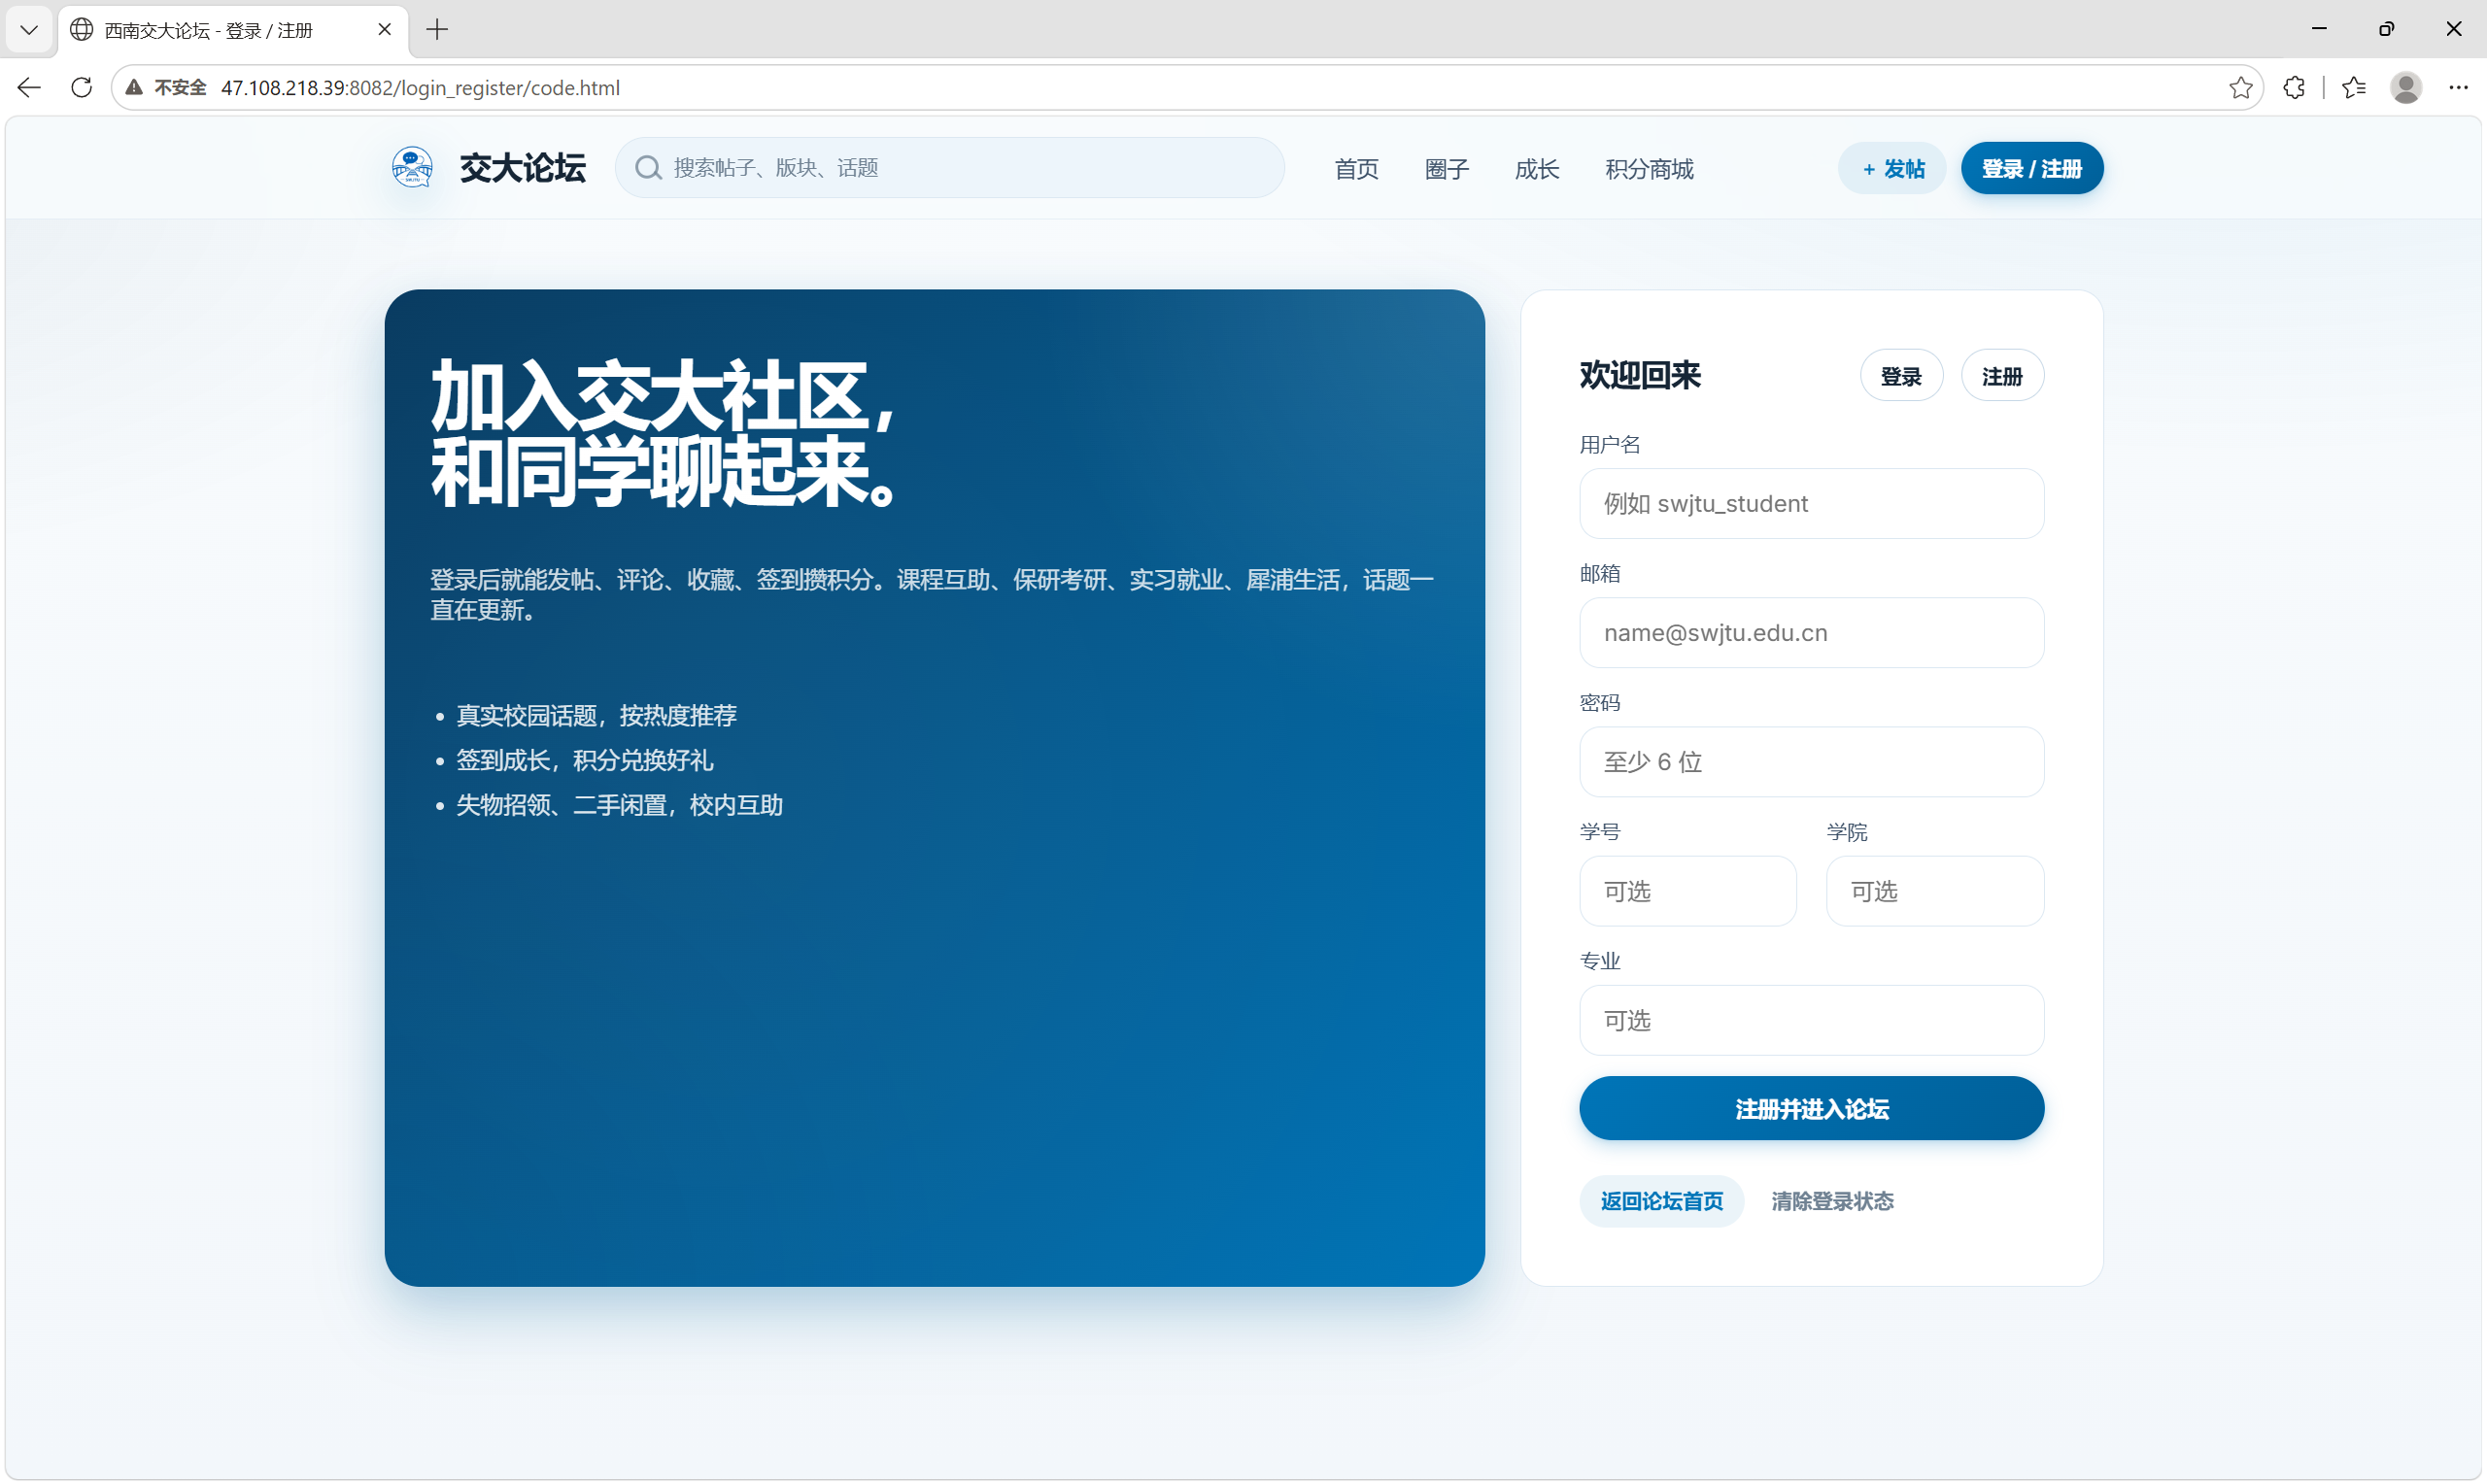
\includegraphics[width=0.85\textwidth]{figures/manual/register_page.png}
    \caption{用户注册页面界面}
    \label{fig:register-page}
\end{figure}

\subsection{用户登录}
已注册用户点击首页右上角「登录 / 注册」按钮，切换至「登录」标签页。登录方式支持：

\begin{itemize}[leftmargin=2em]
    \item \textbf{账号密码登录}：输入用户名和密码，点击「登录进入论坛」。系统校验凭据正确后，生成 JWT Token 并保存到浏览器本地存储，在 Token 有效期内可保持登录状态。
    \item \textbf{登录失败提示}：若用户名不存在、密码错误或表单为空，页面会展示错误提示，用户需检查输入后重新提交。
    \item \textbf{退出登录}：用户可通过导航栏或个人入口执行退出操作，系统会清除本地登录状态并返回未登录视图。
\end{itemize}

登录成功后，页面右上角显示用户头像和昵称，下拉菜单提供「个人中心」「我的帖子」「我的收藏」「通知中心」「退出登录」等入口。



\begin{figure}[!htbp]
    \centering
    \begin{subfigure}{0.48\textwidth}
        \centering
        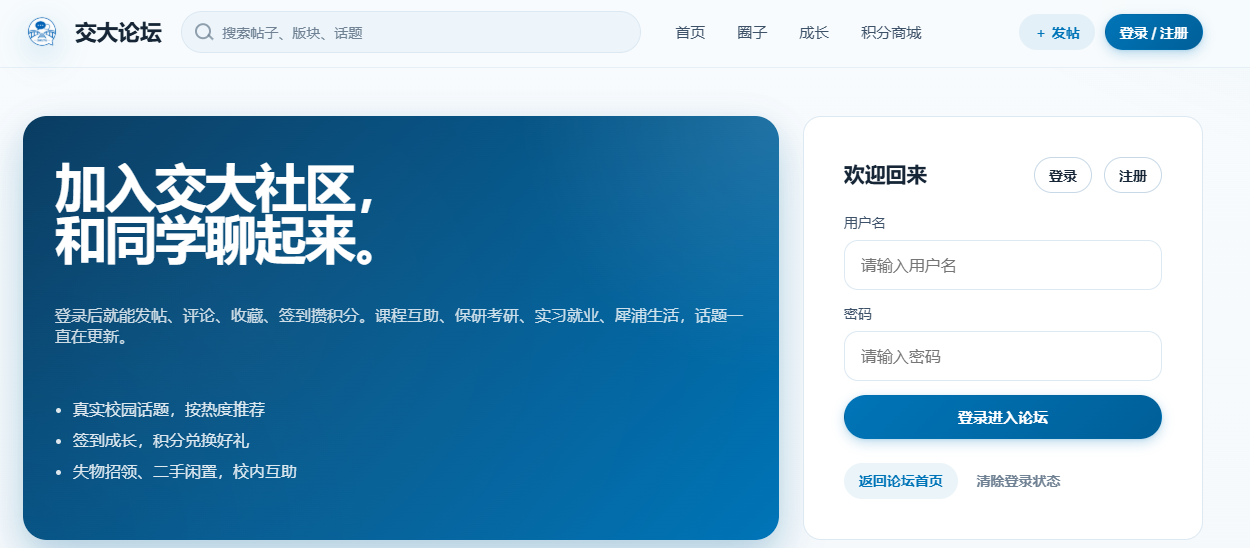
\includegraphics[width=\textwidth]{figures/manual/login_page.png}
        \caption{登录页面}
    \end{subfigure}
    \hfill
    \begin{subfigure}{0.48\textwidth}
        \centering
        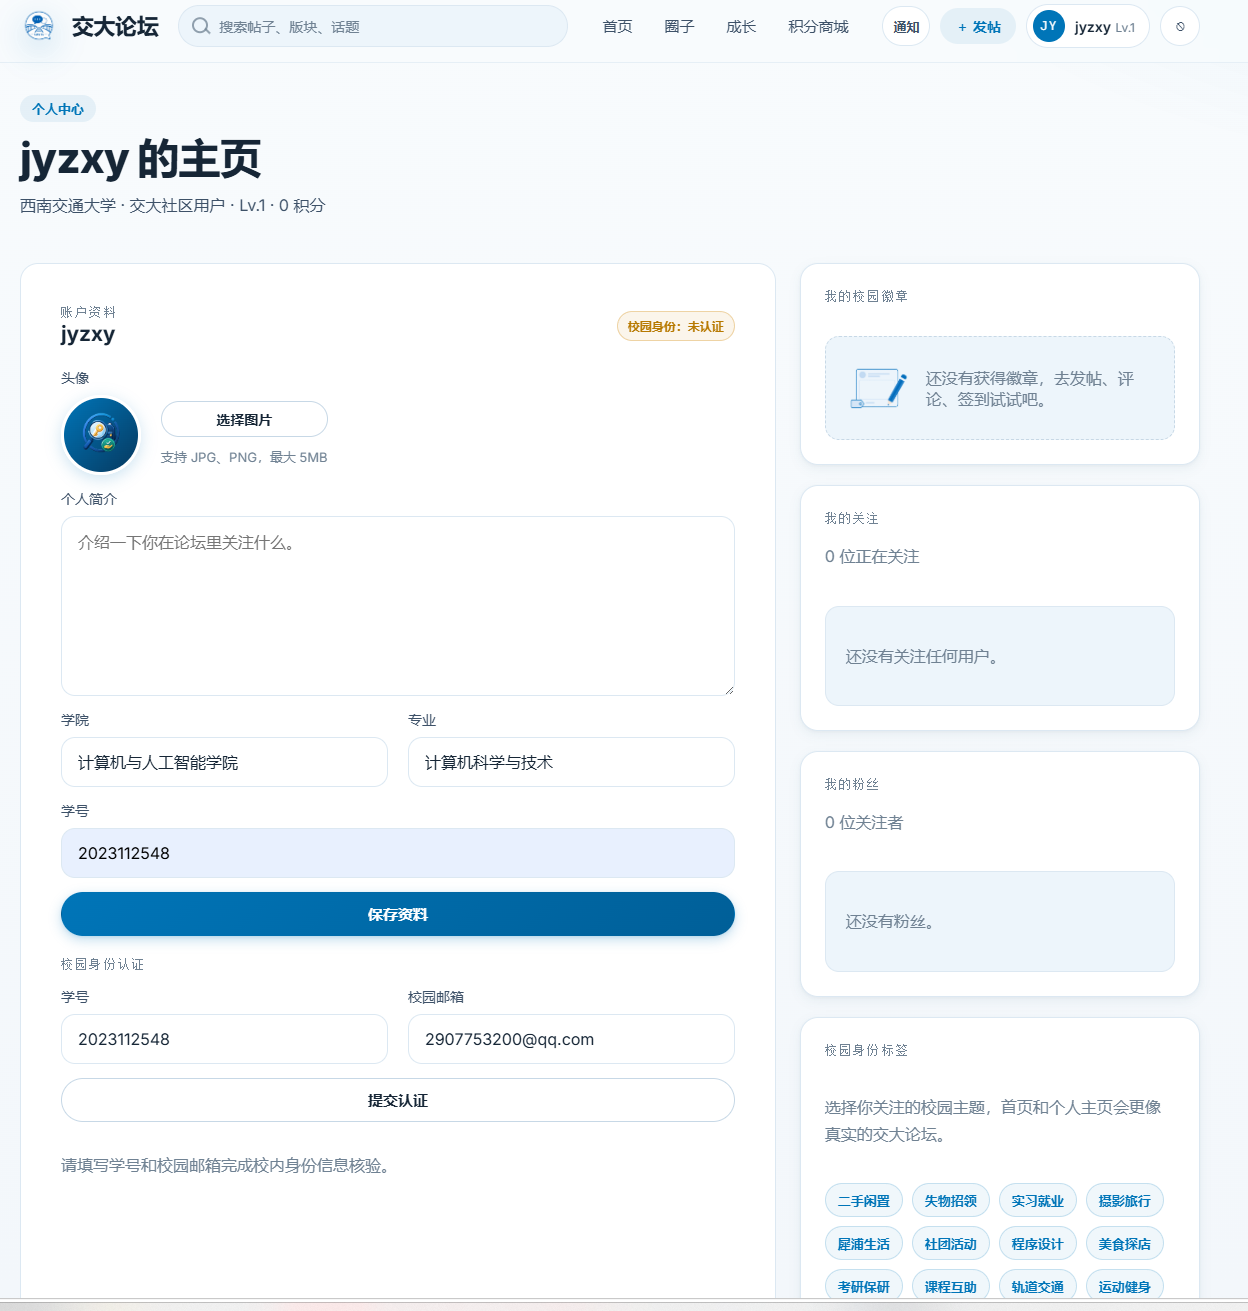
\includegraphics[width=\textwidth]{figures/manual/logged_in_navbar.png}
        \caption{登录后导航栏}
    \end{subfigure}

    \caption{用户登录流程界面}
    \label{fig:login-flow}
\end{figure}



\section{浏览帖子}

\subsection{首页推荐}
进入论坛首页（\url{http://47.108.218.39:8082}），默认展示按热度排序的帖子推荐列表。热度算法综合考虑浏览量、点赞数、评论数、收藏数和发布时间衰减因子，计算公式为：

\begin{equation}
    H = \frac{P \times w_p + C \times w_c + S \times w_s + V \times w_v}{(T_{\text{now}} - T_{\text{post}} + 2)^{\gamma}}
\end{equation}

其中 $P$ 为点赞数，$C$ 为评论数，$S$ 为收藏数，$V$ 为浏览量，$w_p, w_c, w_s, w_v$ 为对应权重系数，$T_{\text{now}} - T_{\text{post}}$ 为帖子发布时间距当前的小时数，$\gamma$ 为时间衰减指数（默认 1.5）。该算法确保新发布且互动活跃的帖子获得更高曝光，同时避免旧帖子长期占据首页。

首页采用瀑布流布局，每行展示 2--3 个帖子卡片，卡片包含：帖子标题（最多 2 行，超出截断并显示省略号）、摘要（前 80 字）、作者头像和昵称、发布时间（相对时间，如「2 小时前」）、版块标签、浏览量/点赞数/评论数统计。点击卡片任意区域进入帖子详情页。


\begin{figure}[!htbp]
    \centering
    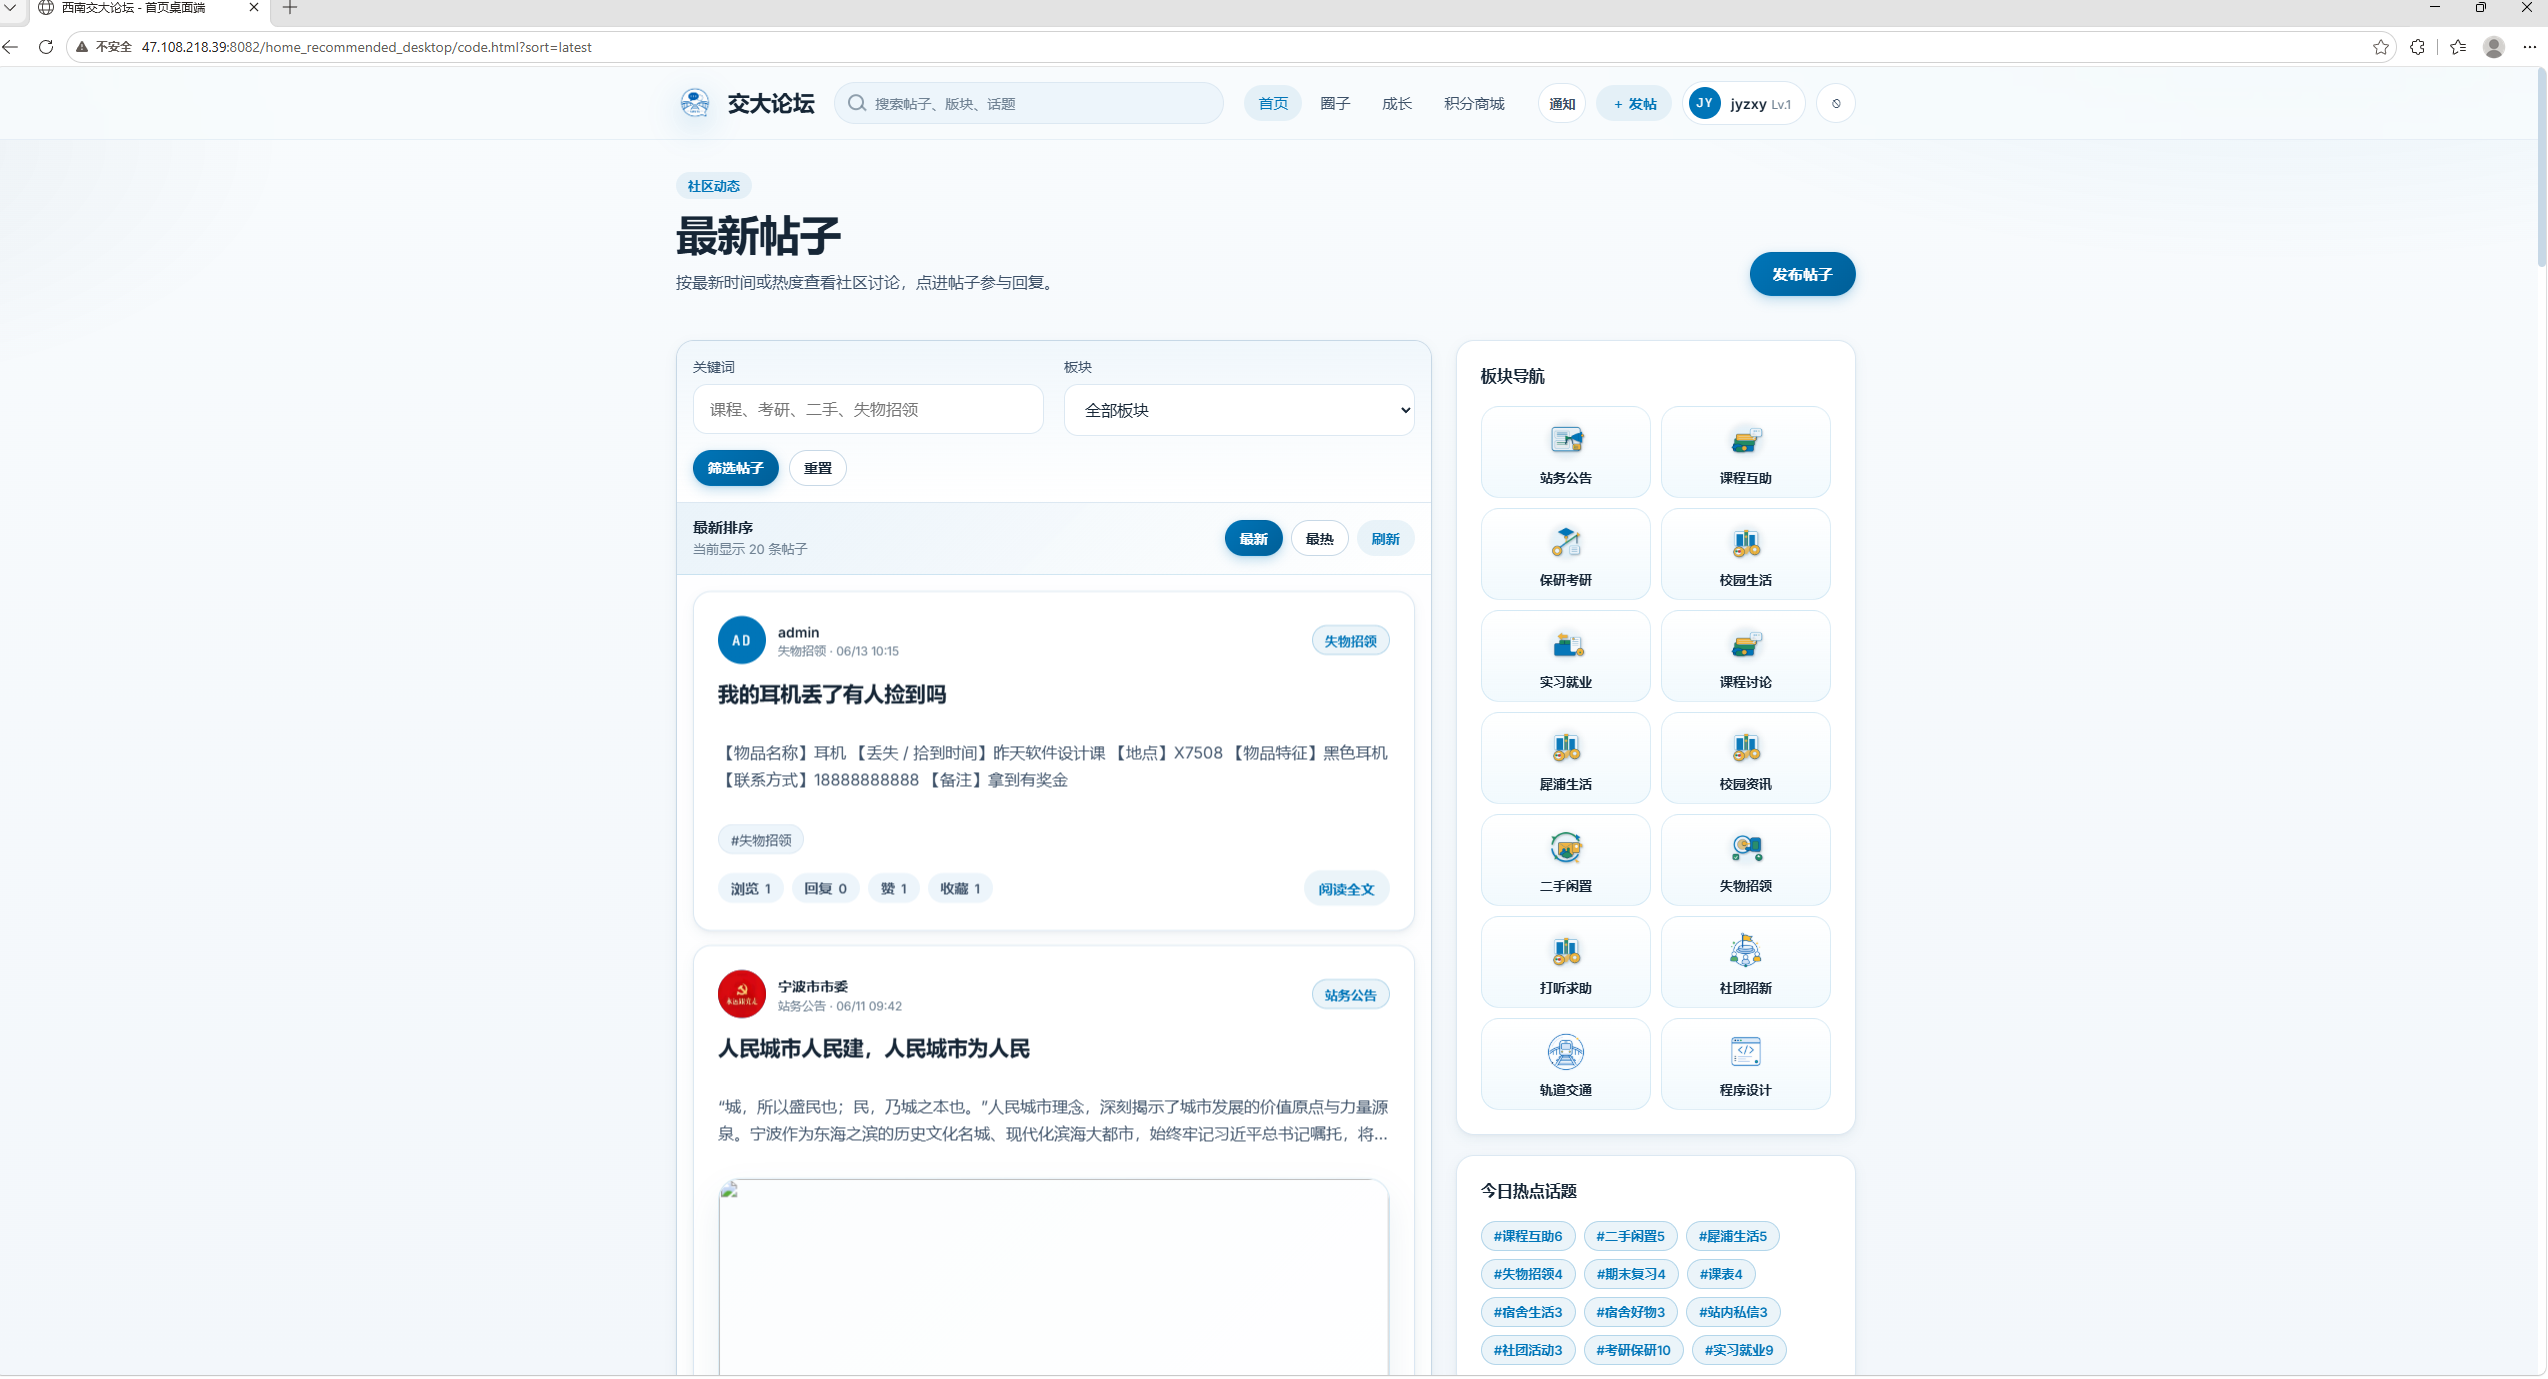
\includegraphics[width=0.92\textwidth]{figures/manual/homepage.png}
    \caption{论坛首页推荐界面}
    \label{fig:homepage}
\end{figure}

\subsection{按版块浏览}
首页右侧提供版块导航栏，当前支持的版块包括：

\begin{table}[!htbp]
    \caption{论坛版块分类说明}
    \label{tab:sections}
    \centering
    \small
    \begin{tabular}{p{0.22\textwidth}p{0.55\textwidth}p{0.12\textwidth}}
        \toprule[1.5pt]
        版块名称 & 内容说明 & 认证要求 \\
        \midrule[1pt]
        课程互助 & 课程资料分享、作业讨论、考试复习交流 & 无 \\
        保研考研 & 保研经验、考研资料、院校选择讨论 & 需认证 \\
        实习就业 & 实习内推、校招信息、面试经验分享 & 需认证 \\
        犀浦生活 & 校园生活、周边美食、活动通知 & 无 \\
        二手闲置 & 教材、电子产品、生活用品交易 & 无 \\
        失物招领 & 失物寻找、拾物归还、寻物启事 & 无 \\
        \bottomrule[1.5pt]
    \end{tabular}
\end{table}

点击版块名称后，页面切换至该版块专属视图，帖子列表仅展示该版块内容，排序方式支持「热度」「最新」「精华」。版块页面顶部显示版块介绍、发帖数统计和关注按钮，关注后该版块新帖将在首页优先展示。



\begin{figure}[!htbp]
    \centering
    \begin{subfigure}{0.48\textwidth}
        \centering
        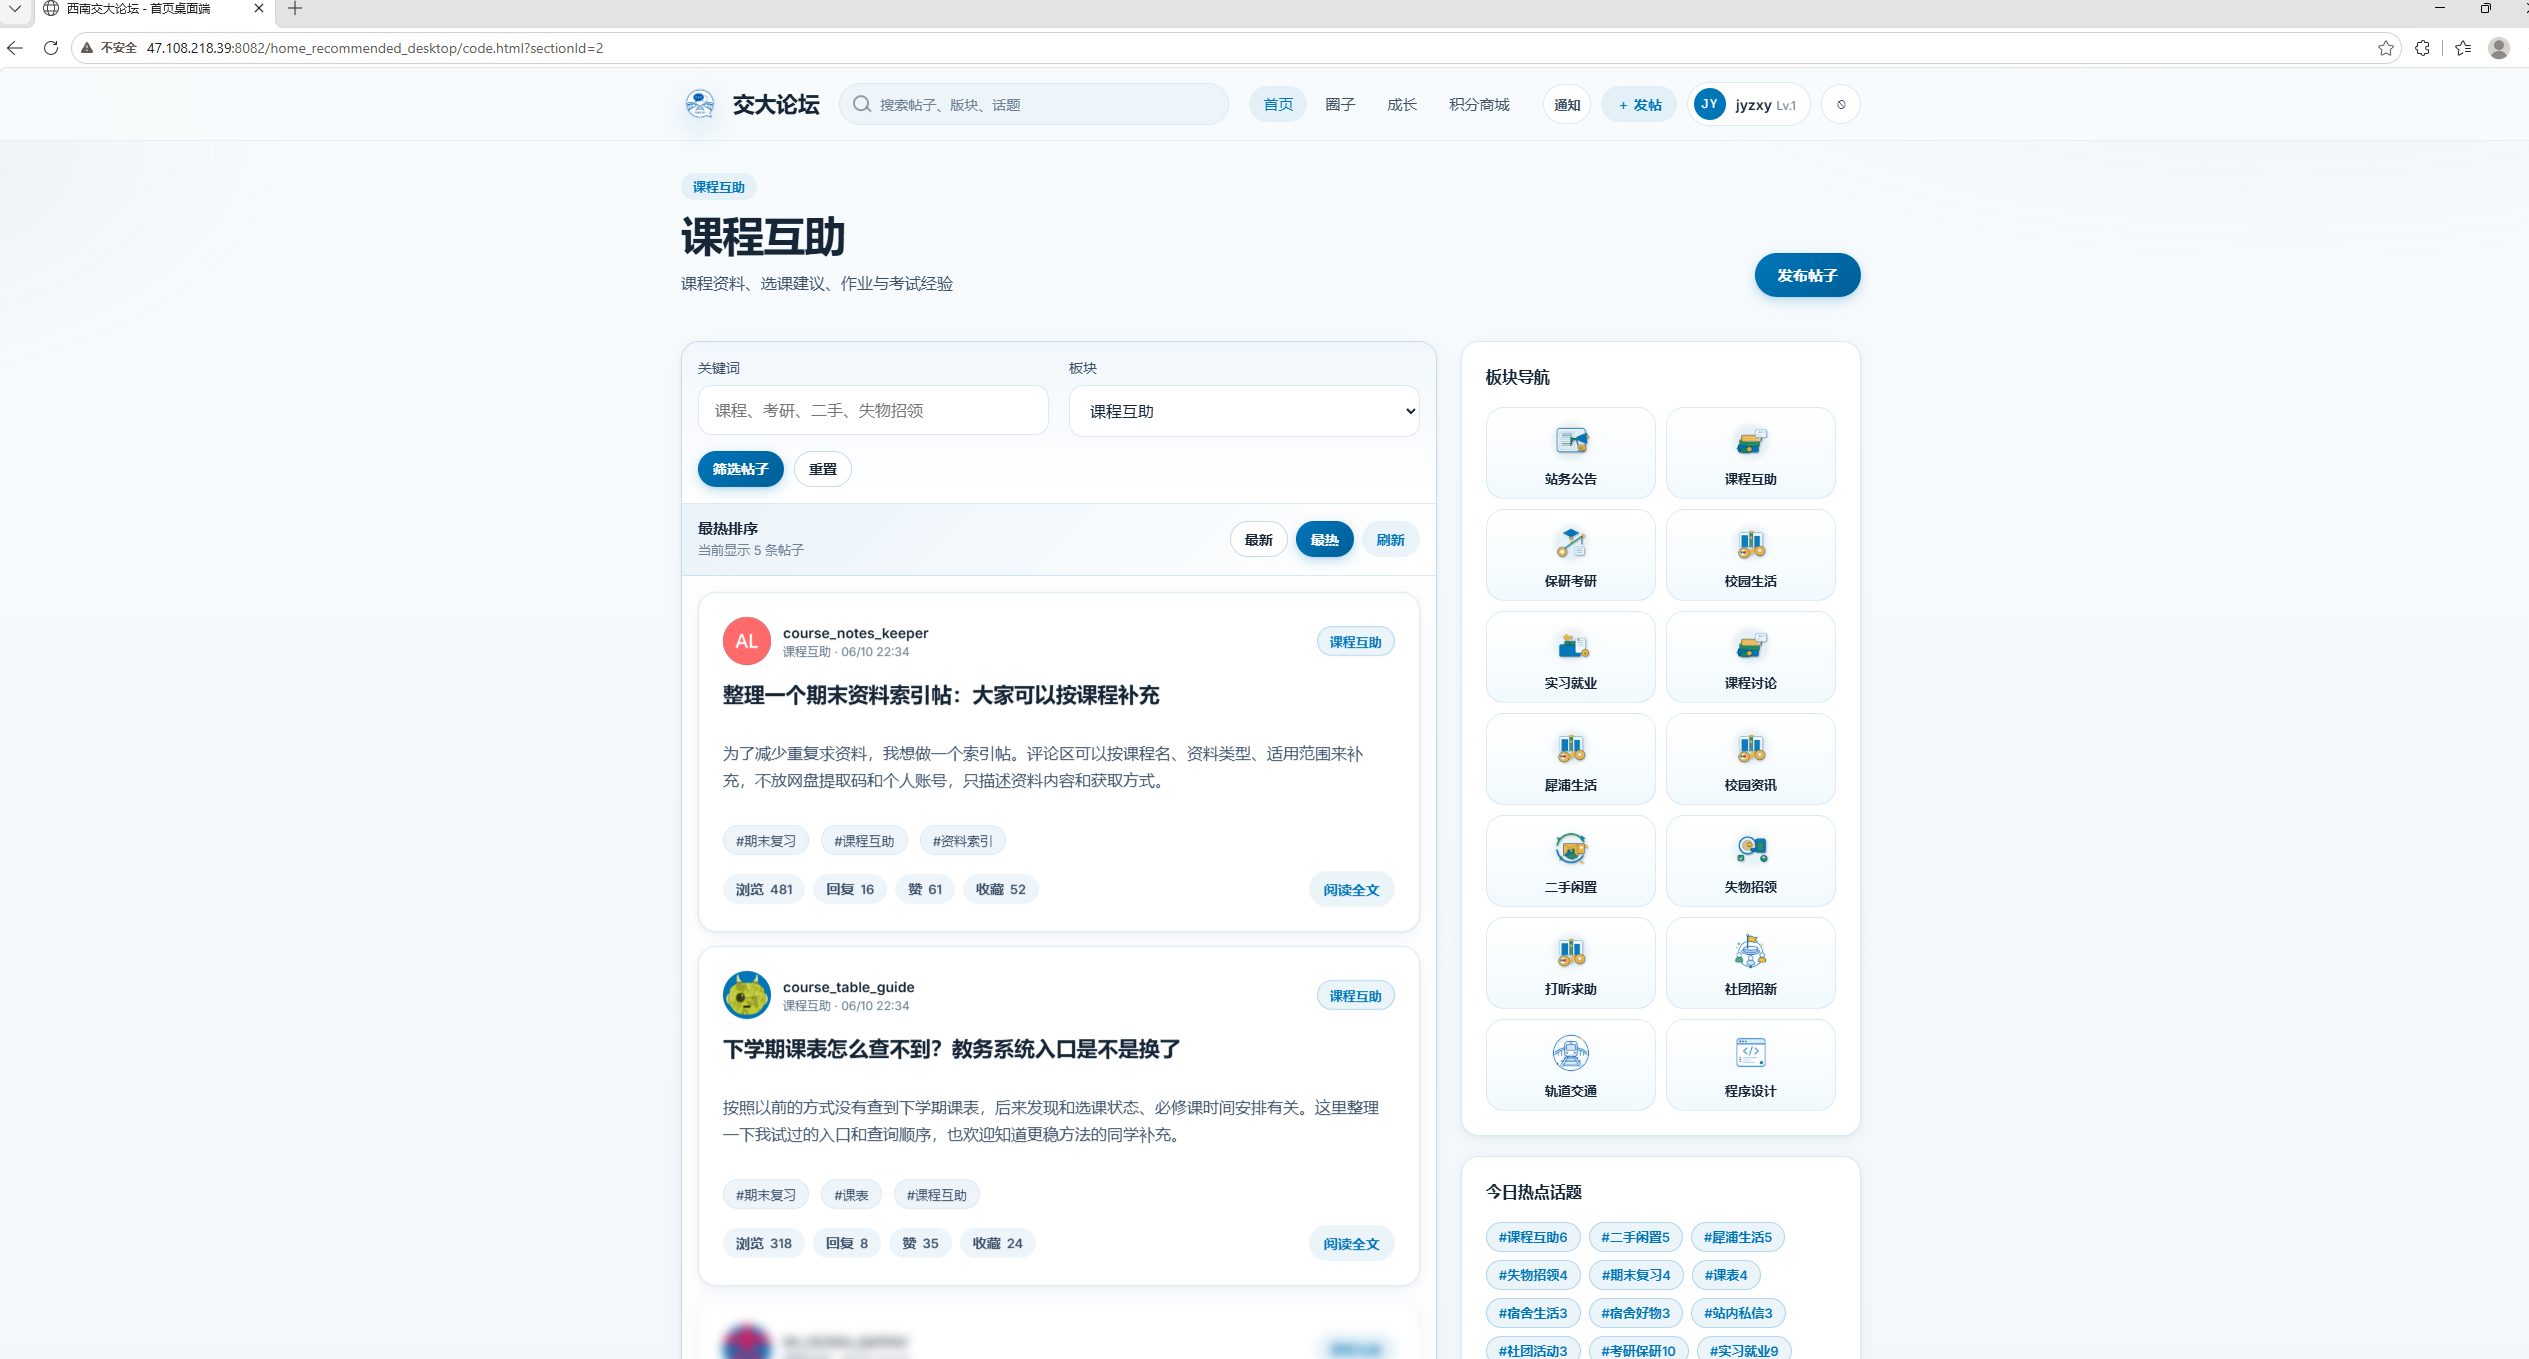
\includegraphics[width=\textwidth]{figures/manual/section_course.png}
        \caption{课程互助版块}
    \end{subfigure}
    \hfill
    \begin{subfigure}{0.48\textwidth}
        \centering
        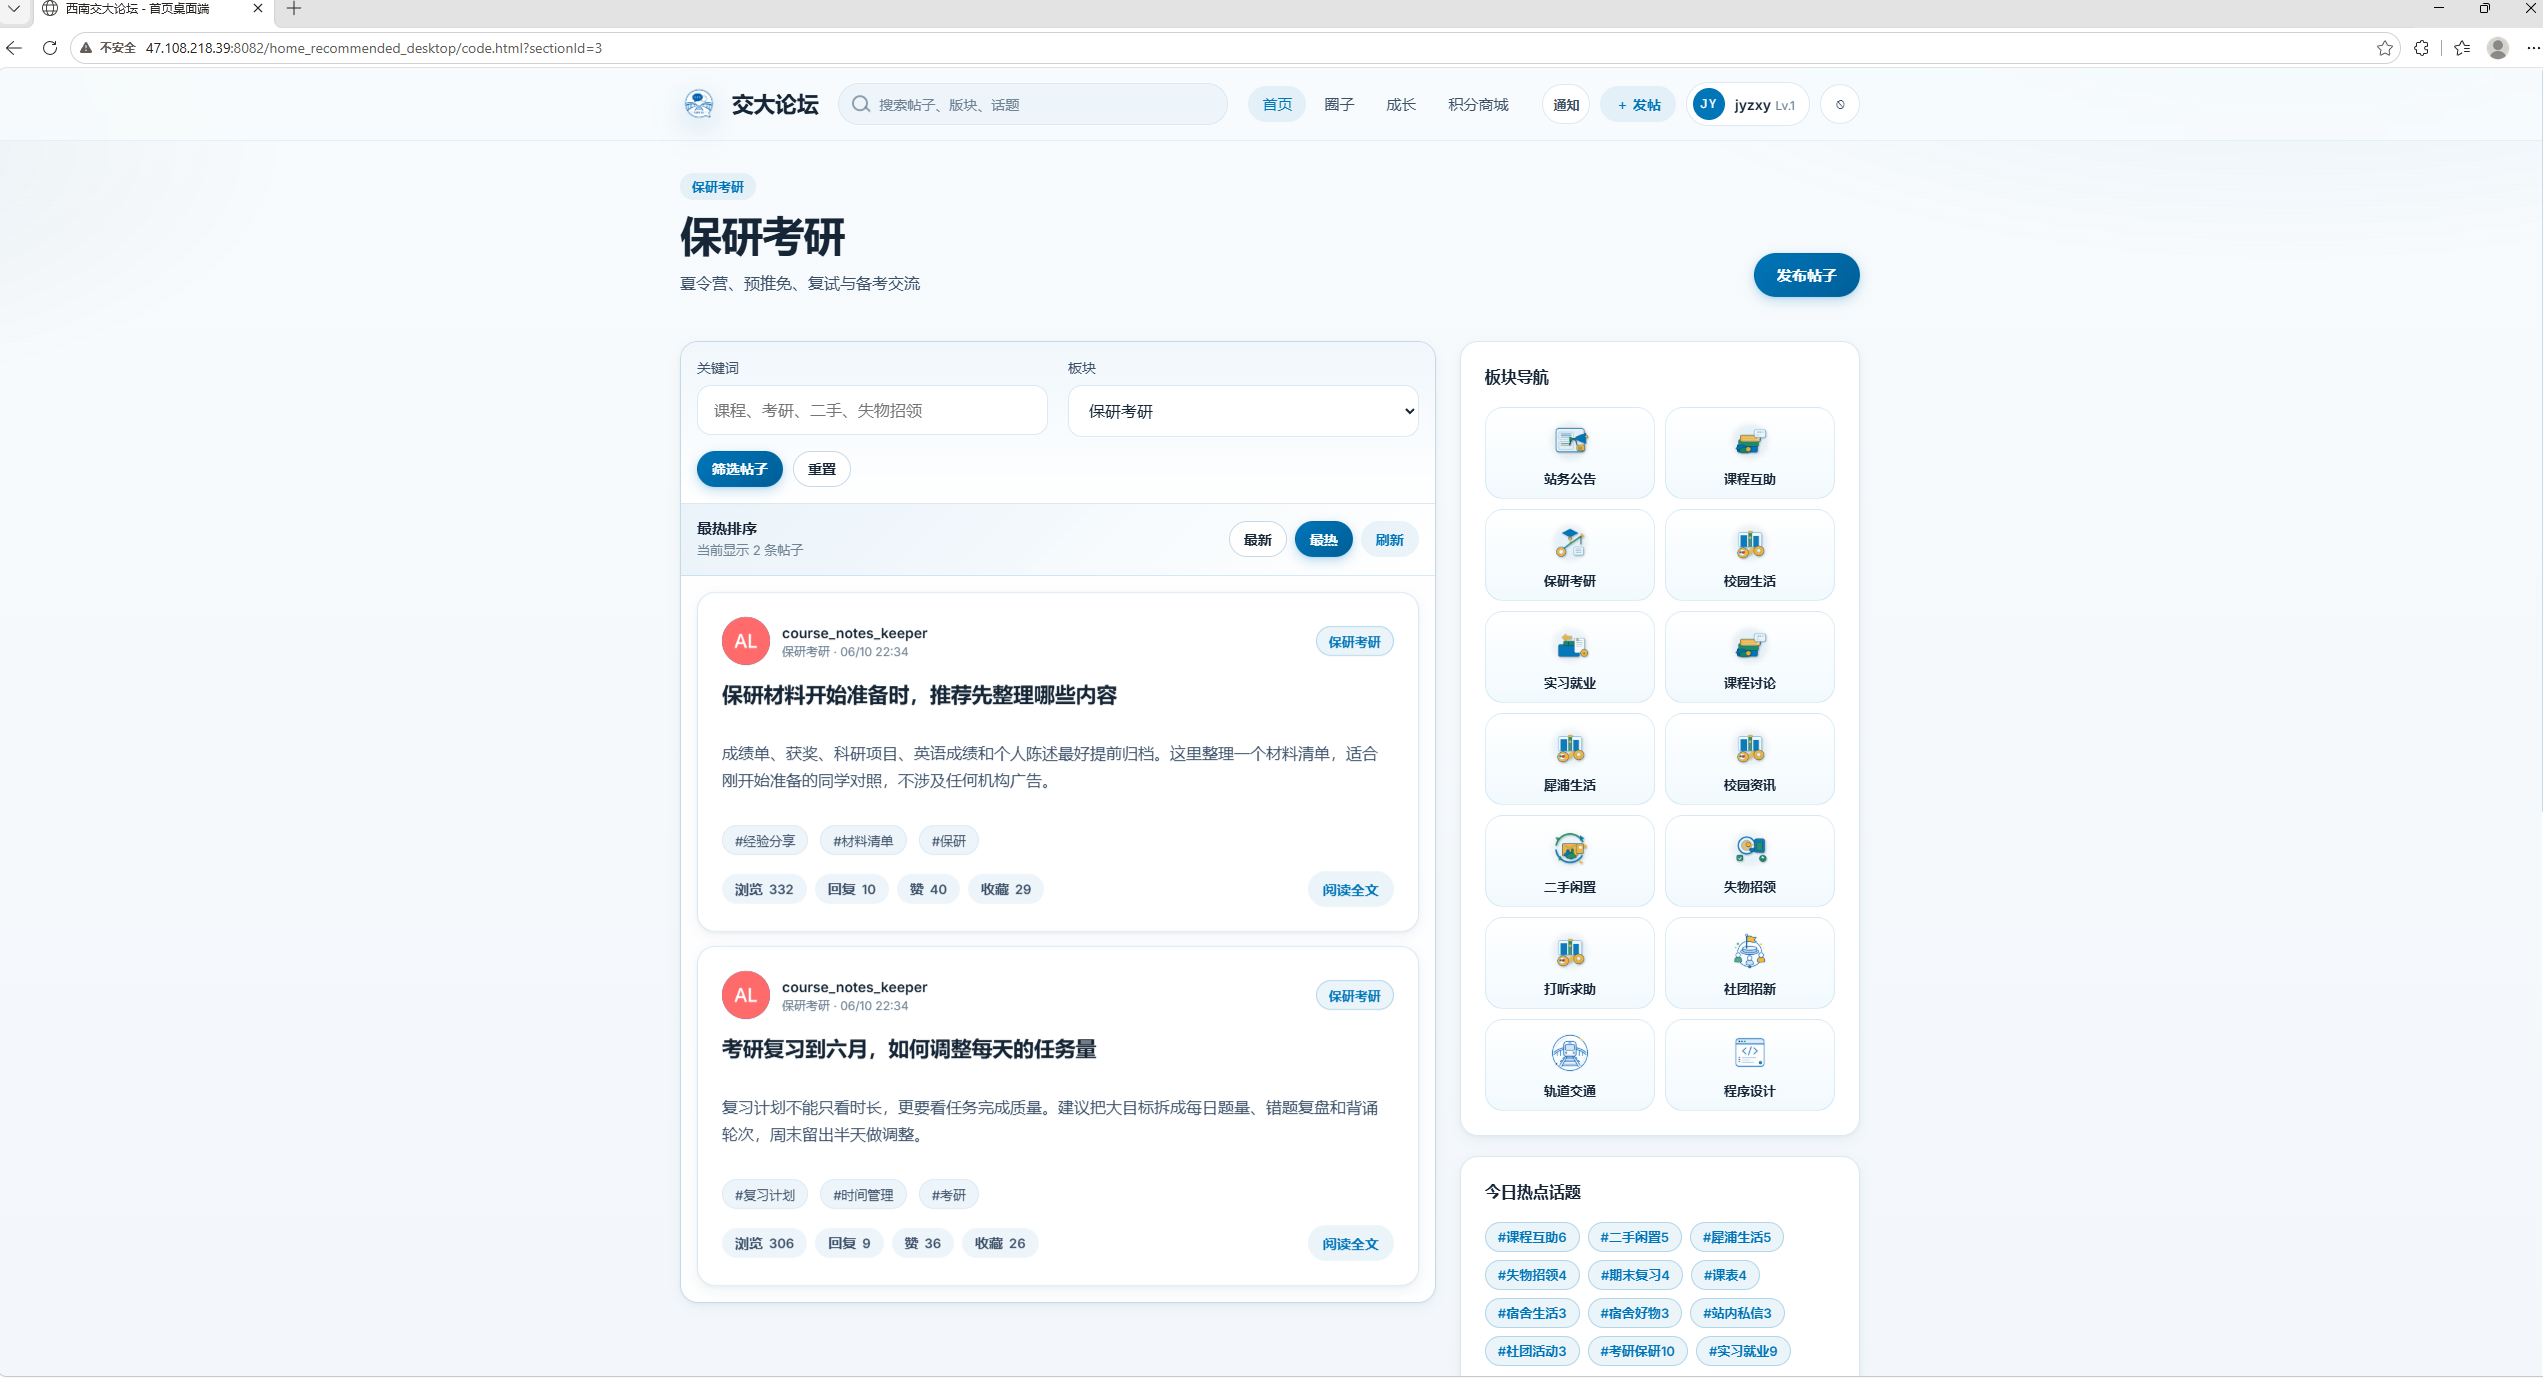
\includegraphics[width=\textwidth]{figures/manual/section_graduate.png}
        \caption{保研考研版块}
    \end{subfigure}
    \caption{不同版块的浏览界面}
    \label{fig:section-browsing}
\end{figure}

\subsection{搜索功能}
页面顶部提供全局搜索框，支持关键词搜索帖子标题和内容。搜索请求由前端提交至后端 REST API，后端根据关键词在帖子标题、正文等字段中查询匹配内容，并将结果返回给前端列表展示。高级搜索支持以下筛选条件：

\begin{itemize}[leftmargin=2em]
    \item \textbf{版块筛选}：下拉选择特定版块，缩小搜索范围
    \item \textbf{时间范围}：选择「最近一天」「最近一周」「最近一月」「全部时间」
    \item \textbf{排序方式}：「相关度优先」「最新发布」「热度最高」
    \item \textbf{作者筛选}：输入用户名，仅搜索该用户发布的帖子
\end{itemize}

搜索结果页展示匹配帖子的标题（关键词高亮显示）、摘要片段、作者信息和匹配度评分。无结果时展示空状态插图和提示文案。



\begin{figure}[!htbp]
    \centering
    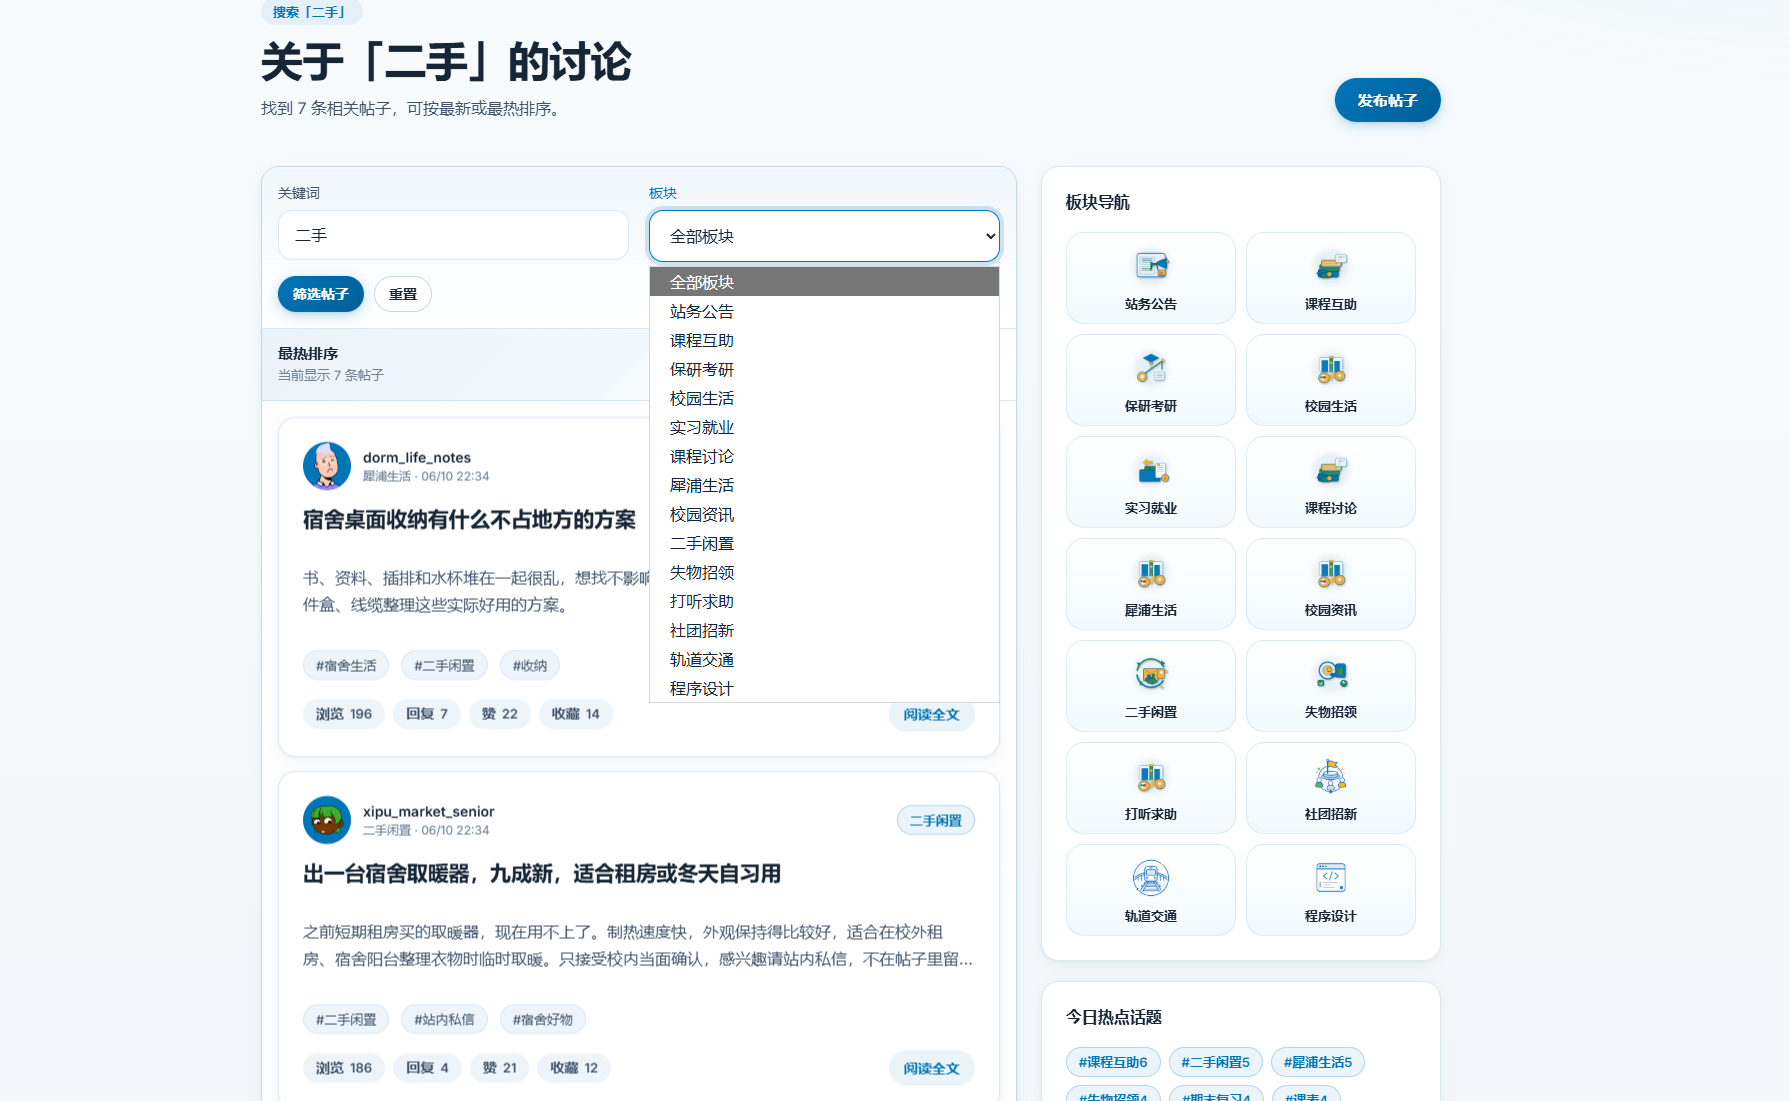
\includegraphics[width=0.92\textwidth]{figures/manual/search_results.png}
    \caption{按话题搜索结果页面界面}
    \label{fig:search-results}
\end{figure}
\begin{figure}[!htbp]
	\centering
	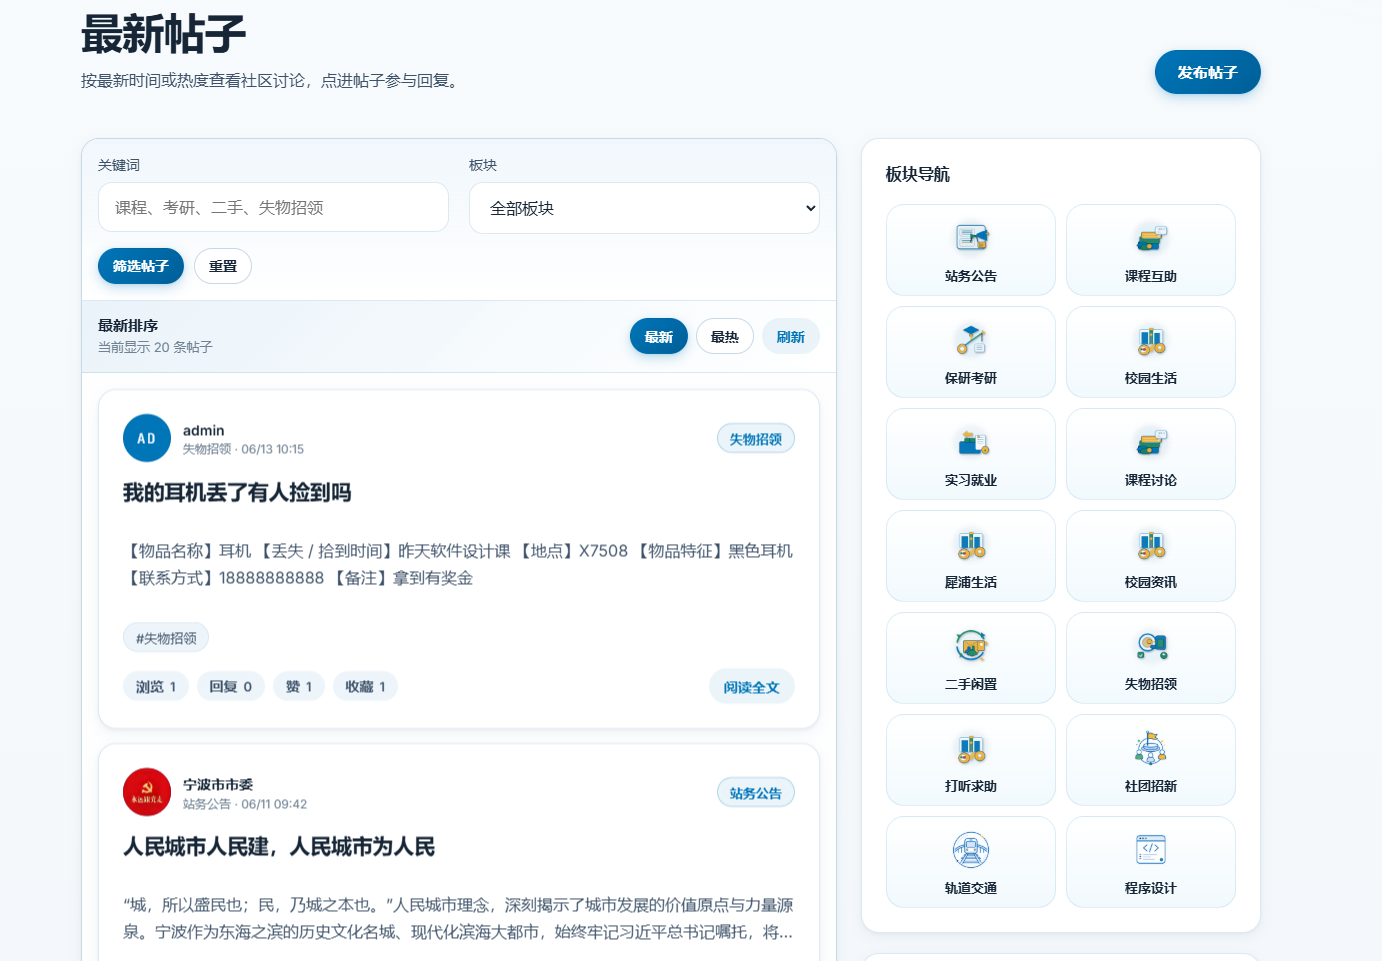
\includegraphics[width=0.92\textwidth]{figures/manual/sort.png}
	\caption{按时间排序结果页面界面}
	\label{fig:search-results-page}
\end{figure}
\begin{figure}[!htbp]
	\centering
	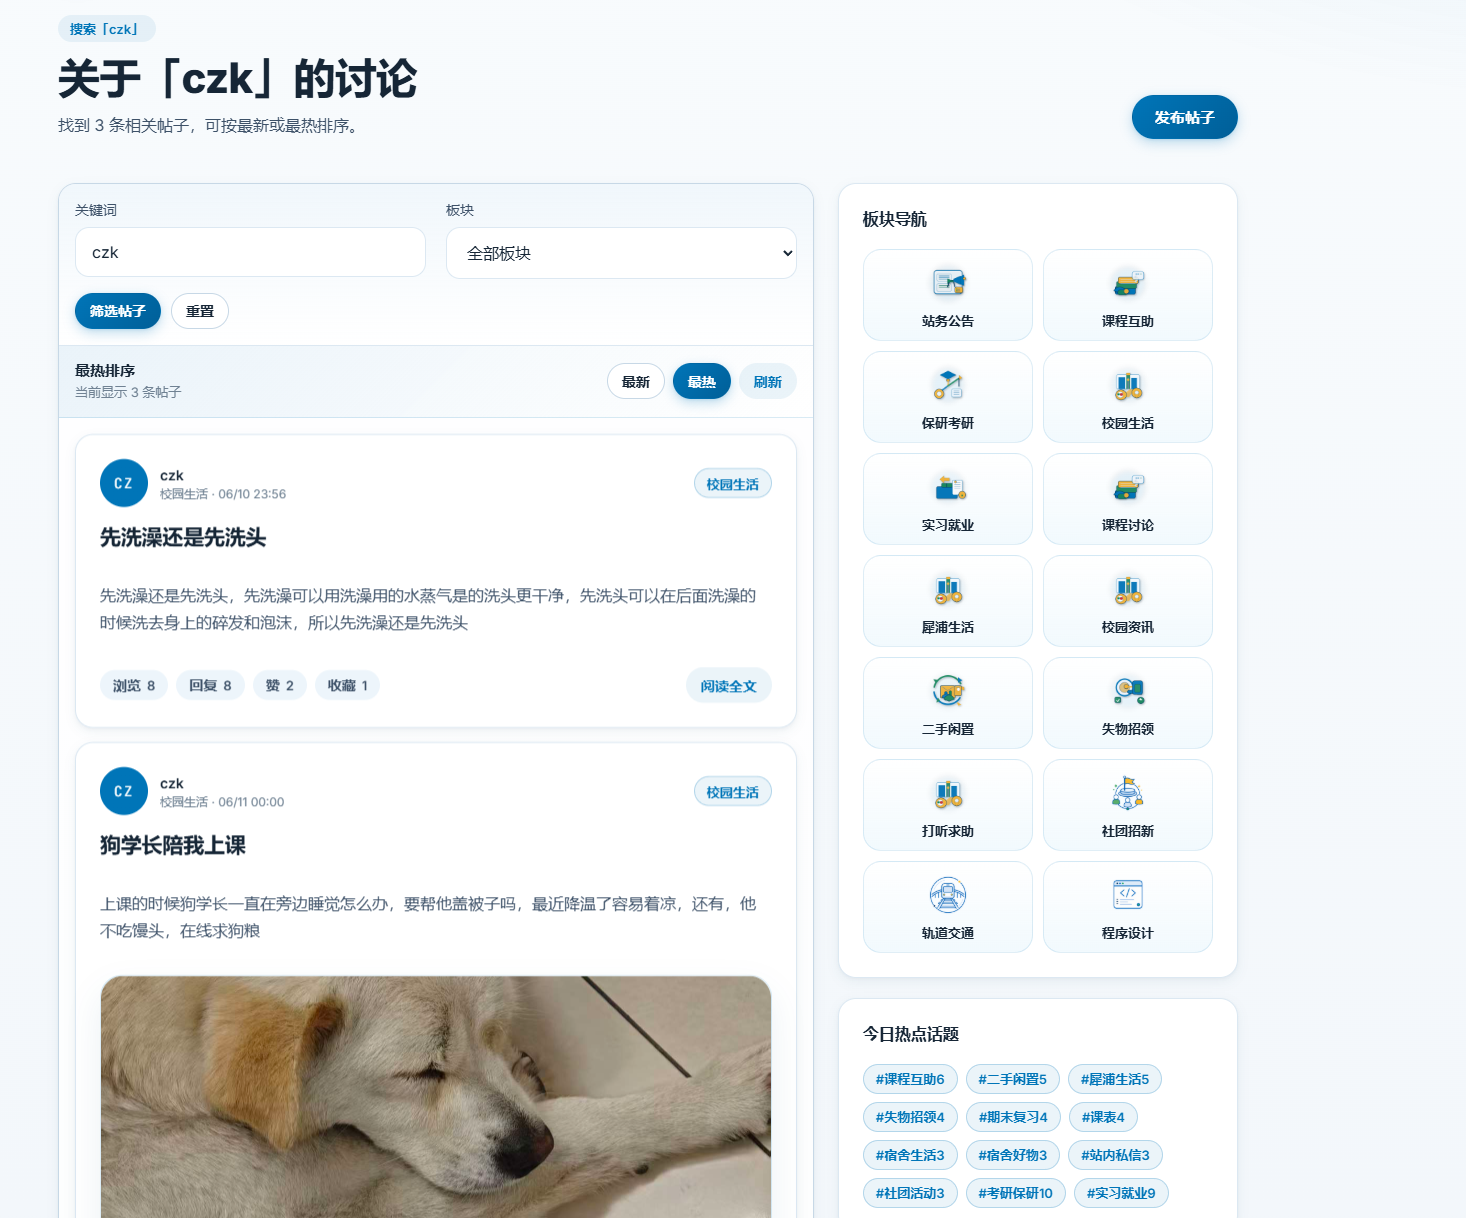
\includegraphics[width=0.92\textwidth]{figures/manual/czk.png}
	\caption{按作者搜索结果页面界面}
	\label{fig:search-results-sort}
\end{figure}
\section{发帖与互动}

\subsection{发布帖子}
点击页面顶部「$+$ 发帖」按钮（或版块页面内的「发布帖子」按钮），进入帖子编辑页面。编辑器采用富文本形式，支持以下功能：

\begin{itemize}[leftmargin=2em]
    \item \textbf{标题}：必填，长度 5--100 个字符，简明概括帖子主题
    \item \textbf{版块}：必填，下拉选择所属版块，决定帖子展示位置和审核策略
    \item \textbf{正文}：必填，支持富文本编辑（加粗、斜体、引用、代码块、有序/无序列表）
    \item \textbf{图片上传}：支持拖拽或点击上传，单张图片不超过 5MB，格式为 JPG/PNG/GIF，最多 9 张
    \item \textbf{标签}：选填，最多添加 5 个标签，用于内容分类和搜索优化，支持输入时自动补全已有标签
    \item \textbf{匿名发布}：选填，勾选后帖子不显示作者真实昵称，显示为「匿名用户」
\end{itemize}

编辑完成后点击「发布」按钮，系统对内容进行敏感词过滤和格式校验。未认证用户发布的帖子进入「待审核」状态，管理员审核通过后在首页展示；已认证用户帖子直接发布。审核通常在 5--30 分钟内完成，用户可在「个人中心 $\rightarrow$ 我的帖子」查看审核状态。


\begin{figure}[!htbp]
    \centering
    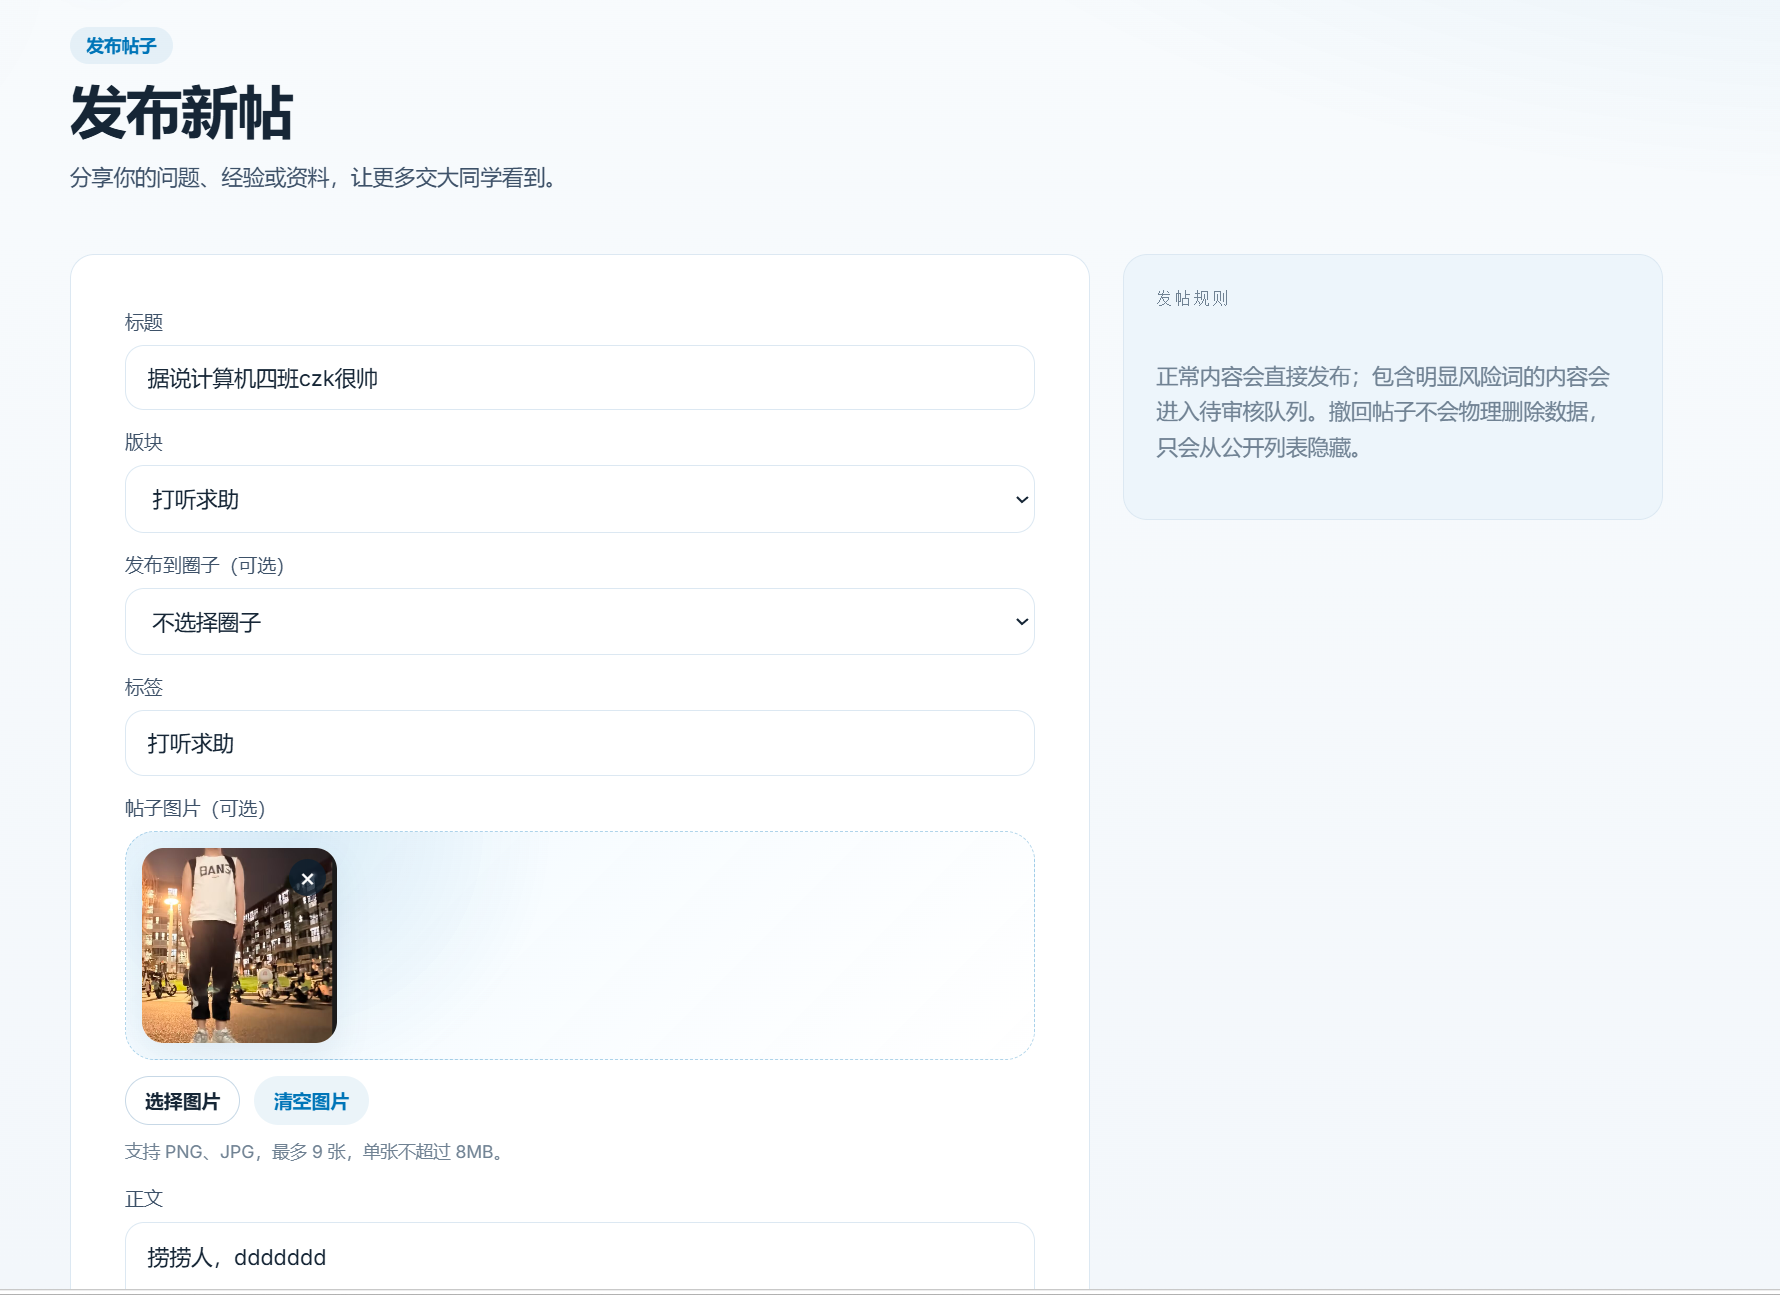
\includegraphics[width=0.92\textwidth]{figures/manual/post_editor.png}
    \caption{帖子发布编辑界面}
    \label{fig:post-editor}
\end{figure}

\subsection{评论与回复}
进入帖子详情页，页面底部为评论输入区域。评论支持以下形式：

\begin{itemize}[leftmargin=2em]
    \item \textbf{一级评论}：直接针对帖子内容发表看法，支持富文本（同发帖编辑器）和图片上传
    \item \textbf{回复评论}：点击某条评论的「回复」按钮，评论框自动引用该评论作者并缩进显示，形成讨论层级
    \item \textbf{点赞评论}：点击评论右侧的「赞」按钮，点赞数实时更新，已点赞状态高亮显示
    \item \textbf{举报评论}：点击「举报」按钮，选择举报原因（垃圾广告、人身攻击、违法违规、其他），提交后管理员处理
\end{itemize}

评论按时间倒序排列（默认）或按热度排序（点赞数优先），用户可切换排序方式。评论数超过 50 条时采用分页加载，每页 20 条，支持「加载更多」按钮或无限滚动。

\textbf{截图指导 8}：请截取帖子详情页的评论区域，展示至少 3--4 条评论（包含一级评论和回复评论），以及评论输入框、排序选项和点赞按钮。确保展示评论层级缩进效果。

\begin{figure}[!htbp]
    \centering
    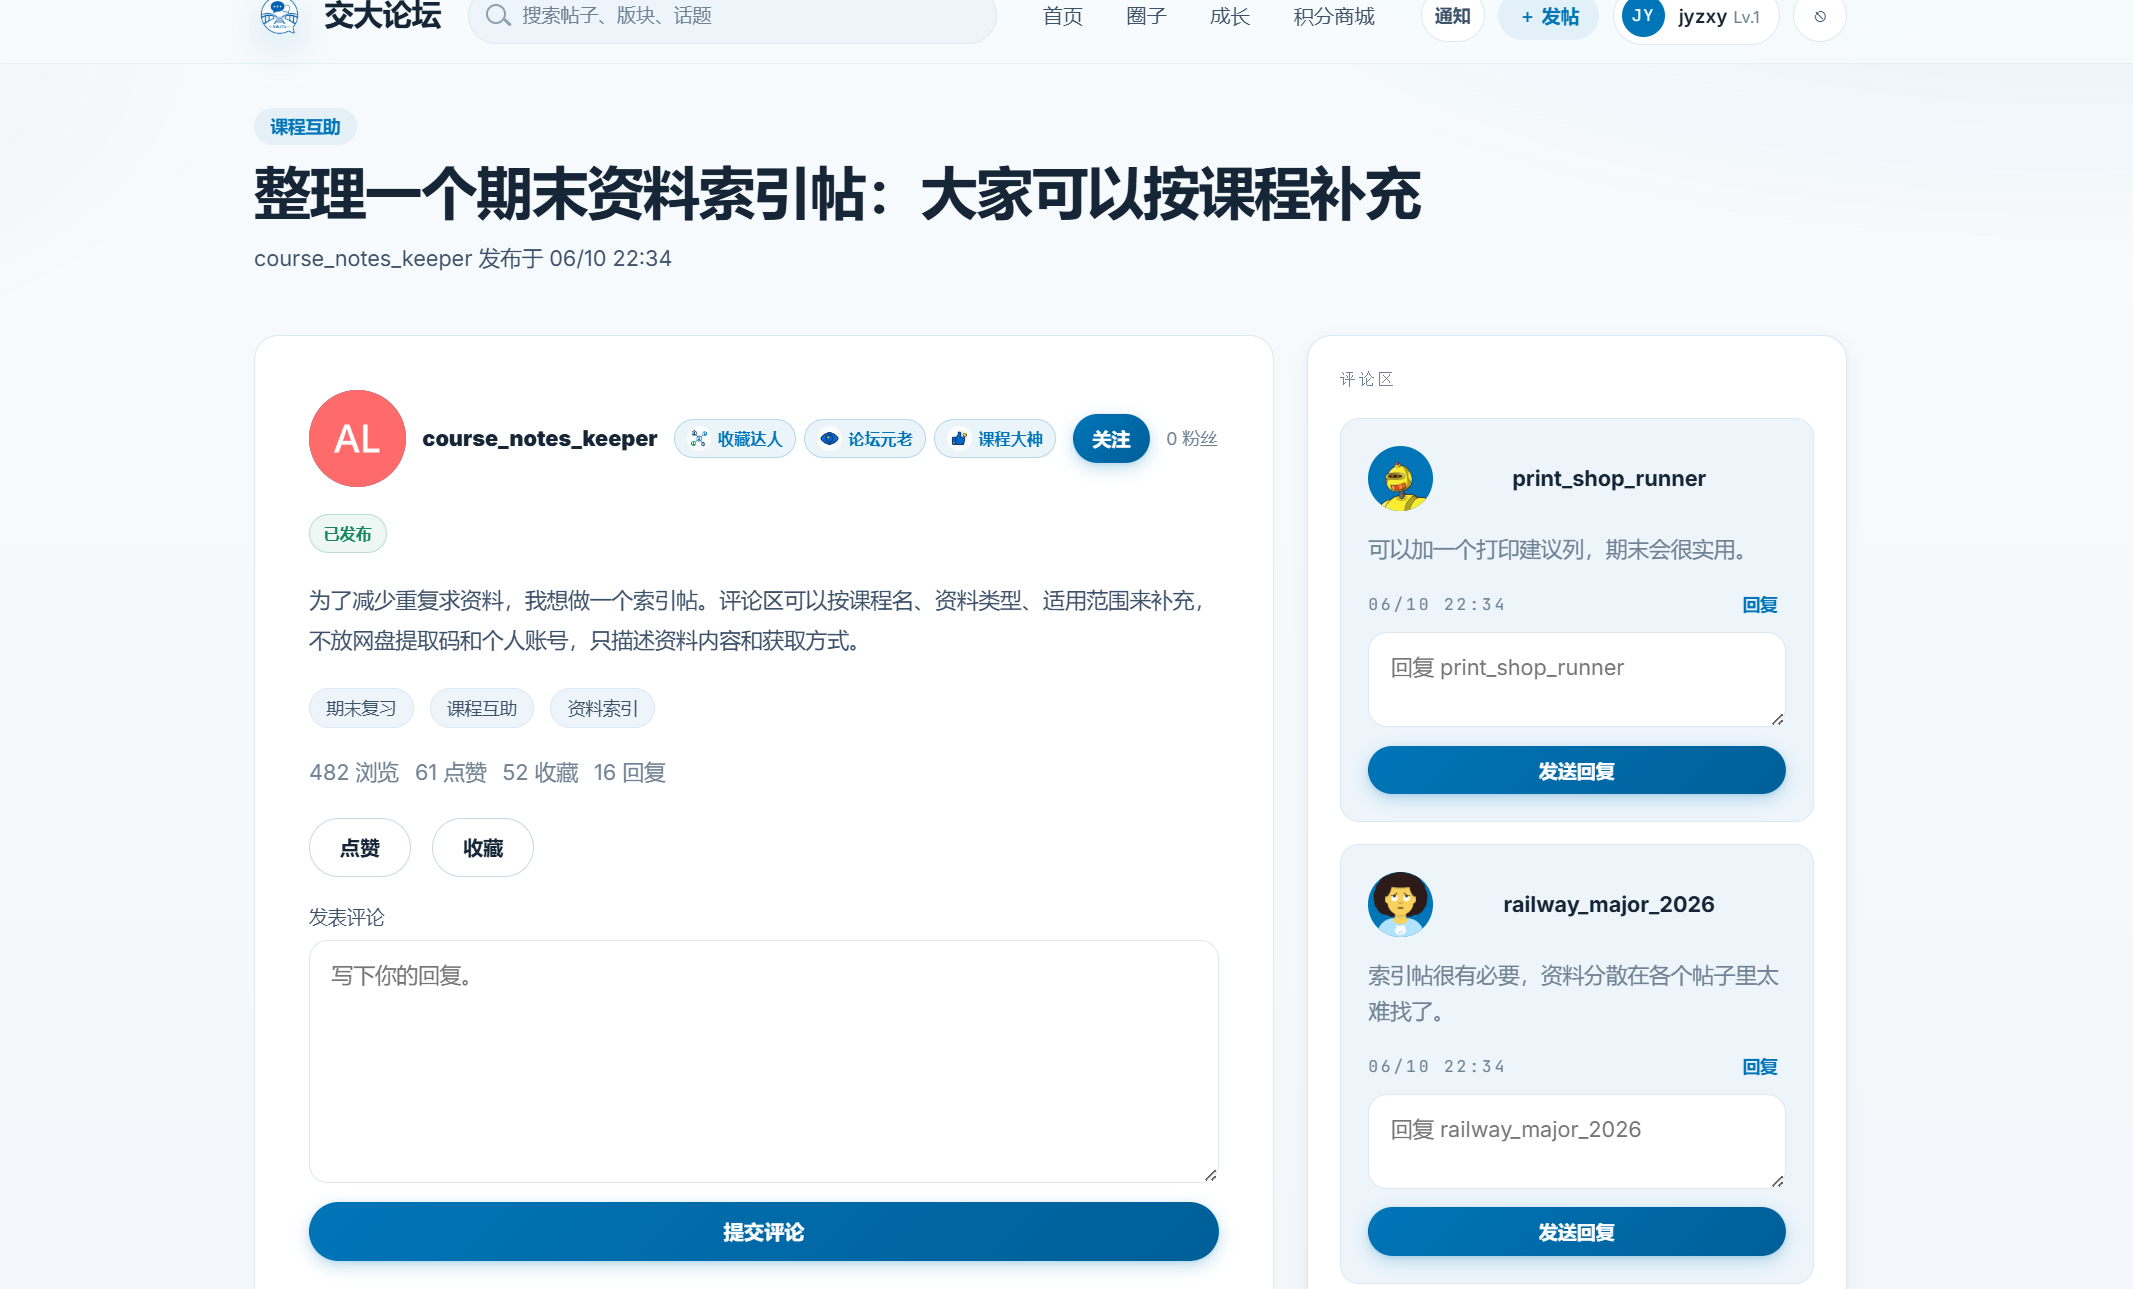
\includegraphics[width=0.92\textwidth]{figures/manual/comment_section.png}
    \caption{帖子评论与回复区域}
    \label{fig:comment-section}
\end{figure}

\subsection{点赞与收藏}
帖子详情页和列表卡片均提供「赞」和「收藏」按钮：

\begin{itemize}[leftmargin=2em]
    \item \textbf{点赞}：点击后按钮变为已激活状态（颜色变化 + 动画效果），点赞数 $+1$；再次点击取消点赞。点赞数据实时同步至服务器，刷新页面后状态保持。
    \item \textbf{收藏}：点击后帖子加入「我的收藏」，收藏按钮变为已激活状态；在个人中心「我的收藏」页面可查看所有收藏帖子，支持按时间排序和取消收藏。
\end{itemize}

点赞和收藏行为均会触发用户行为日志记录，用于首页推荐算法的兴趣匹配计算。



\begin{figure}[!htbp]
    \centering
    \begin{subfigure}{0.48\textwidth}
        \centering
        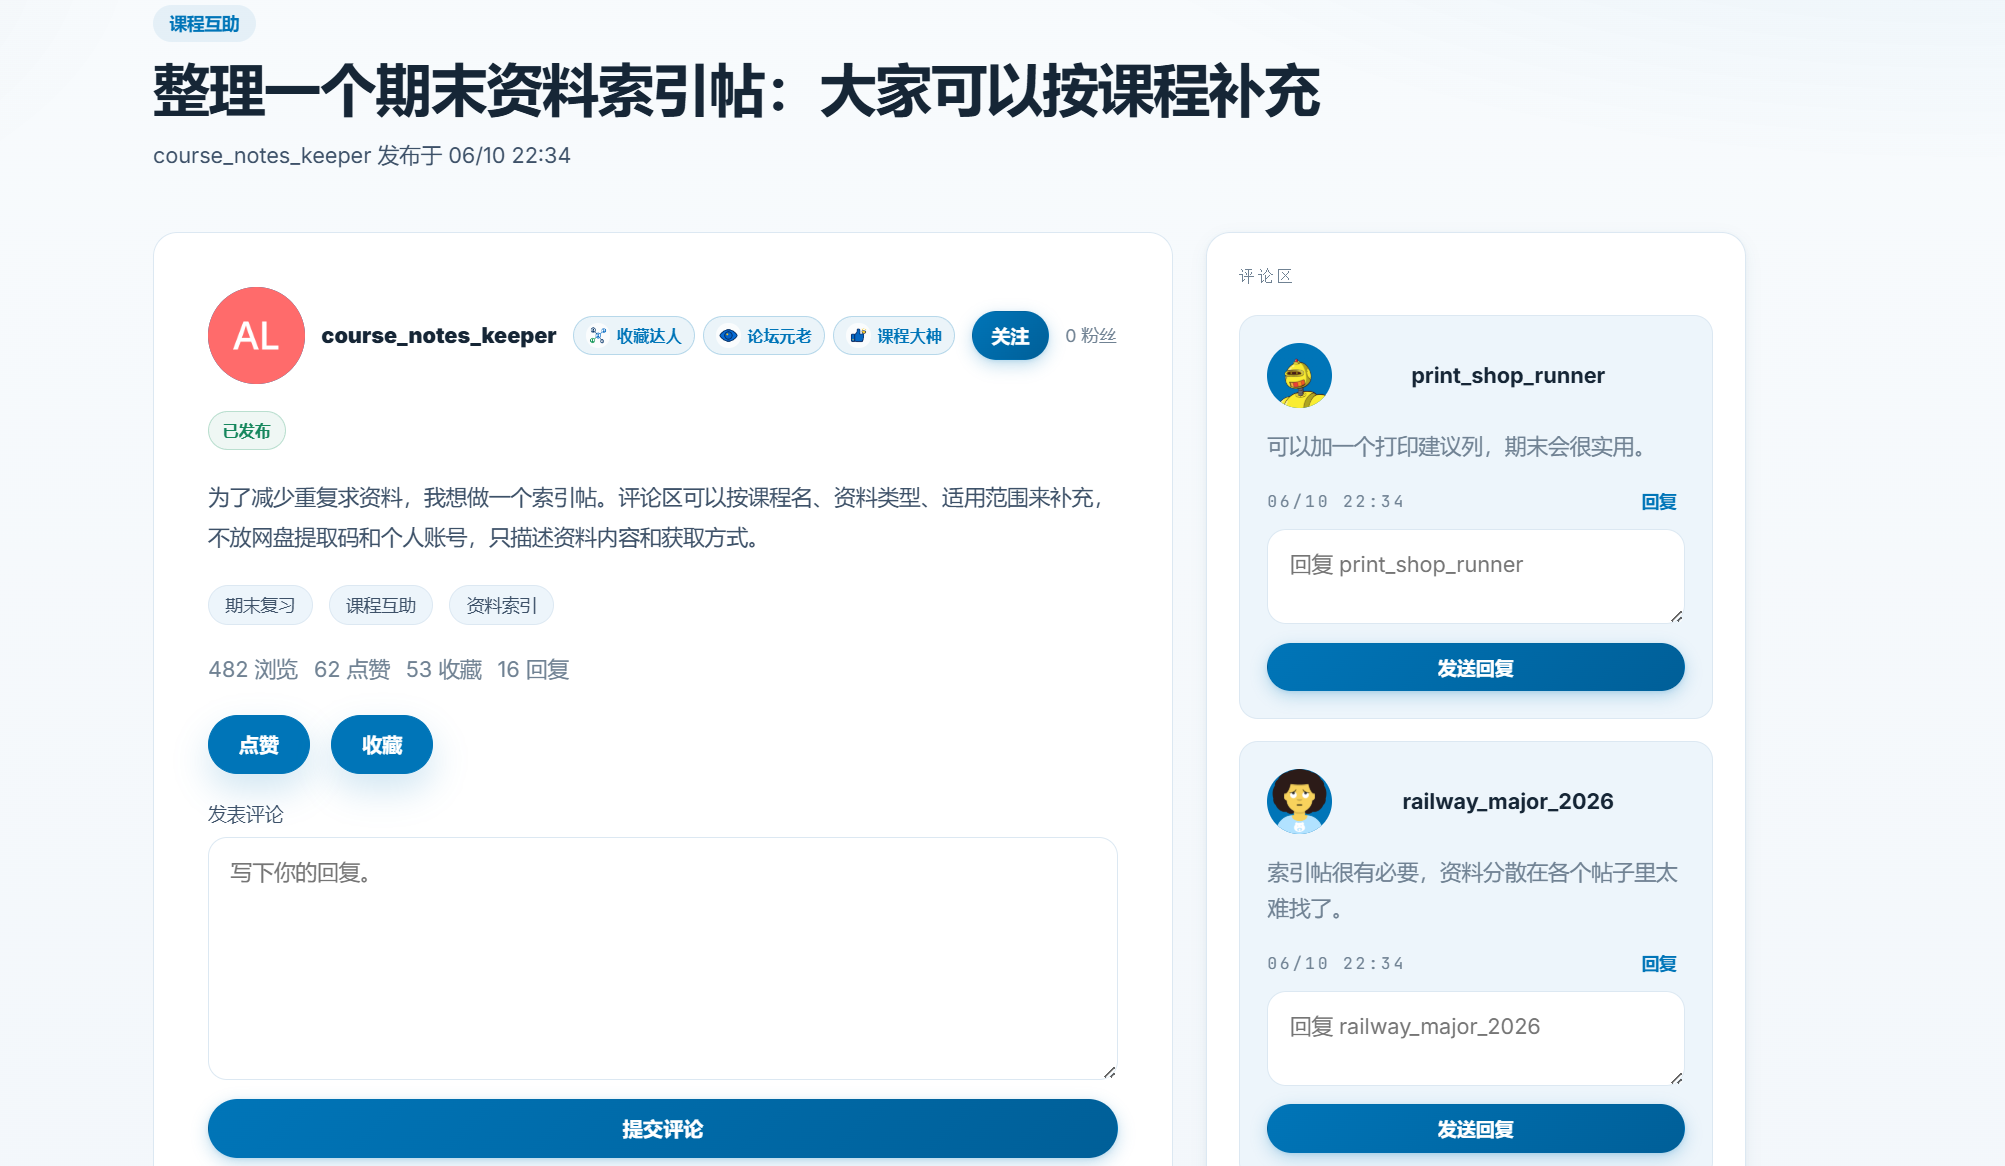
\includegraphics[width=\textwidth]{figures/manual/like_collect_buttons.png}
        \caption{点赞与收藏按钮状态}
    \end{subfigure}
    \hfill
    \begin{subfigure}{0.48\textwidth}
        \centering
        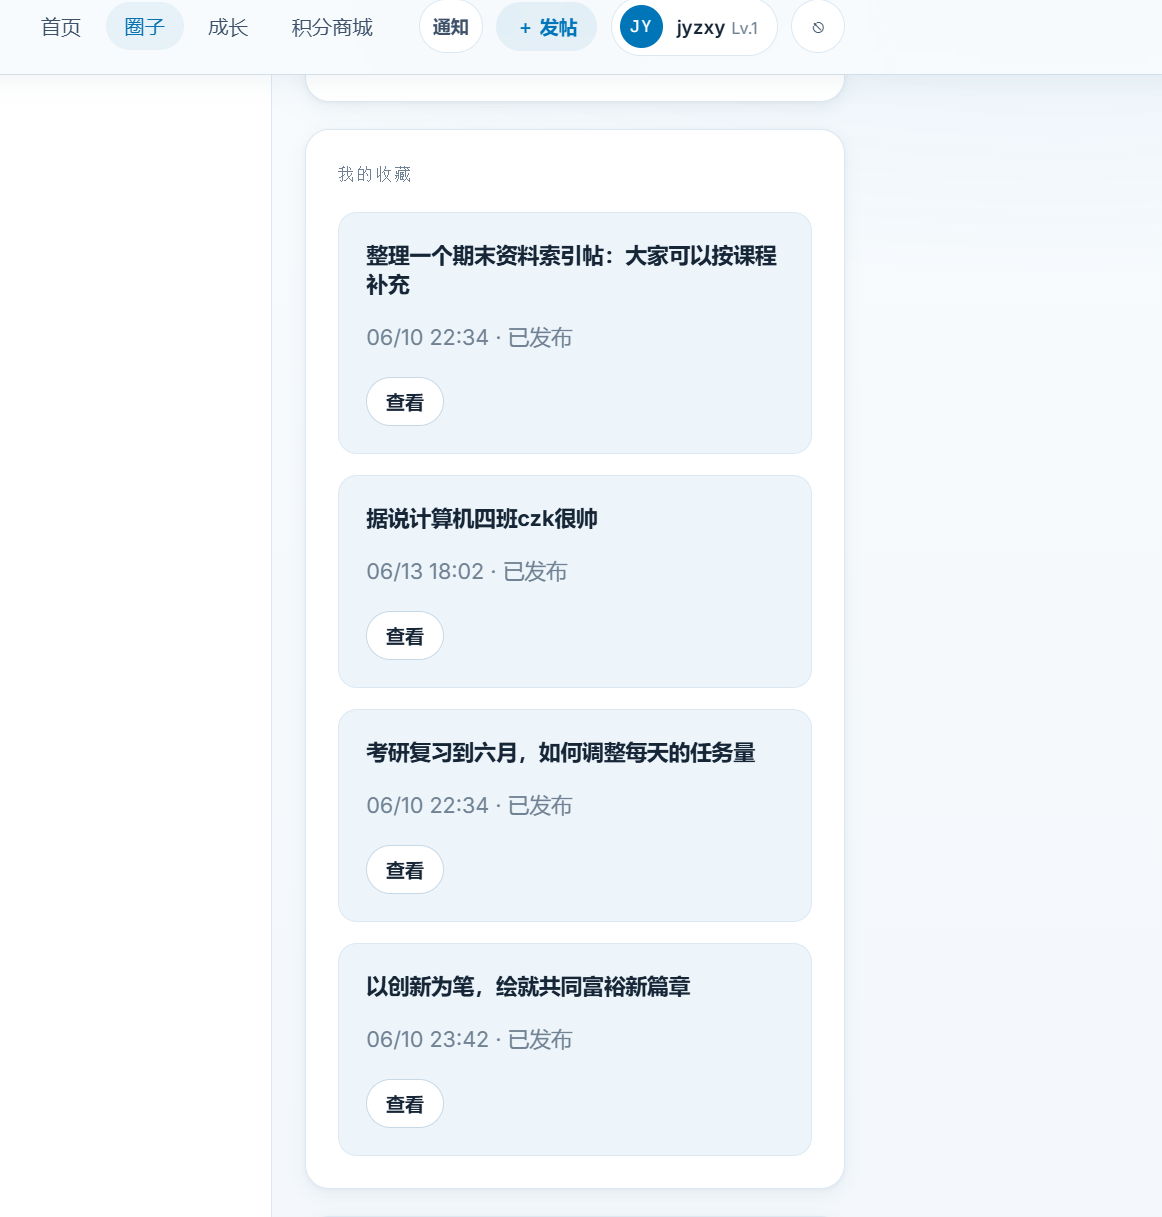
\includegraphics[width=\textwidth]{figures/manual/my_collections.png}
        \caption{我的收藏页面}
    \end{subfigure}
    \caption{点赞与收藏功能界面}
    \label{fig:like-collect}
\end{figure}

\subsection{浏览记录}
系统自动记录用户最近浏览的帖子（最多 50 条），存储于本地存储（LocalStorage）中，无需登录即可记录。登录后浏览记录同步至服务器，实现跨设备同步。用户可在「个人中心 $\rightarrow$ 浏览记录」查看历史浏览列表。

\begin{figure}[!htbp]
    \centering
    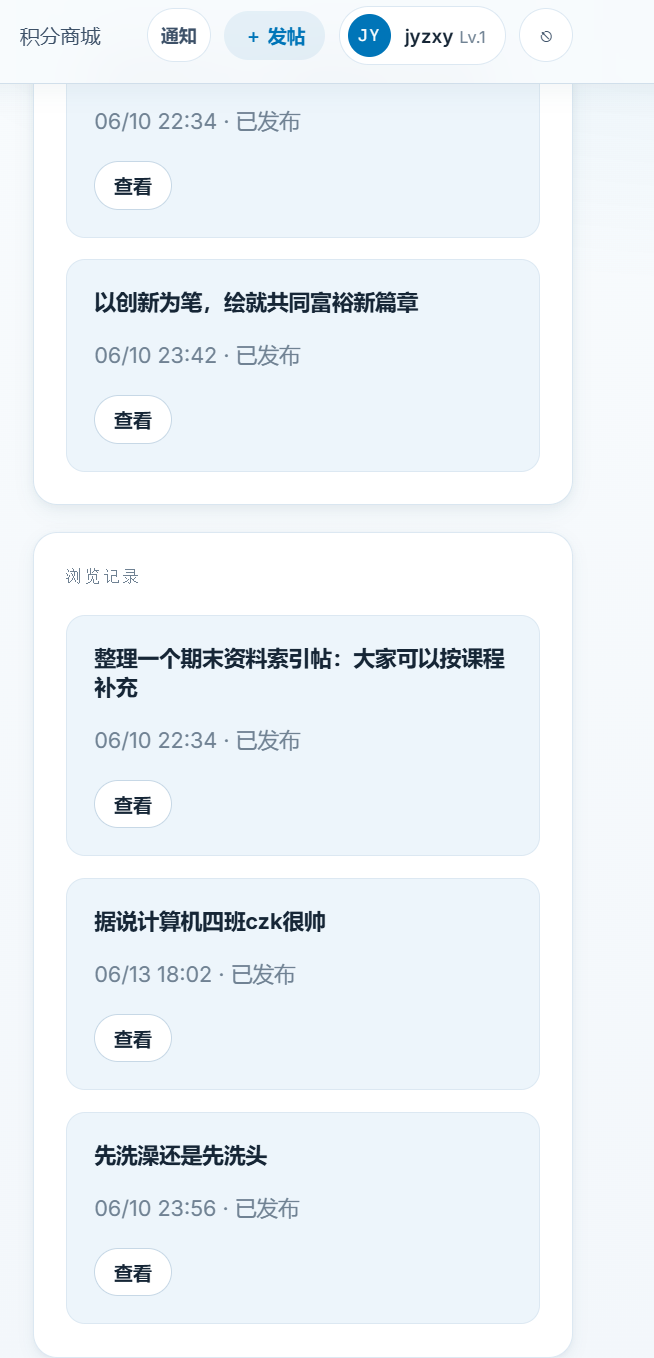
\includegraphics[width=0.85\textwidth]{figures/manual/browsing_history.png}
    \caption{浏览记录页面}
    \label{fig:browsing-history}
\end{figure}

\section{成长与积分}

\subsection{每日签到}
进入「成长中心」页面（顶部导航栏「成长中心」入口或侧边栏快捷入口），点击「今日签到」按钮完成签到。签到规则如下：

\begin{itemize}[leftmargin=2em]
    \item \textbf{基础签到}：每日签到获得 10 积分和 5 经验值，每个账号每天只能签到一次
    \item \textbf{连续签到}：系统自动维护连续签到天数，并在成就模块展示连续签到 7 天、30 天等目标进度
\end{itemize}





\begin{figure}[!htbp]
    \centering
    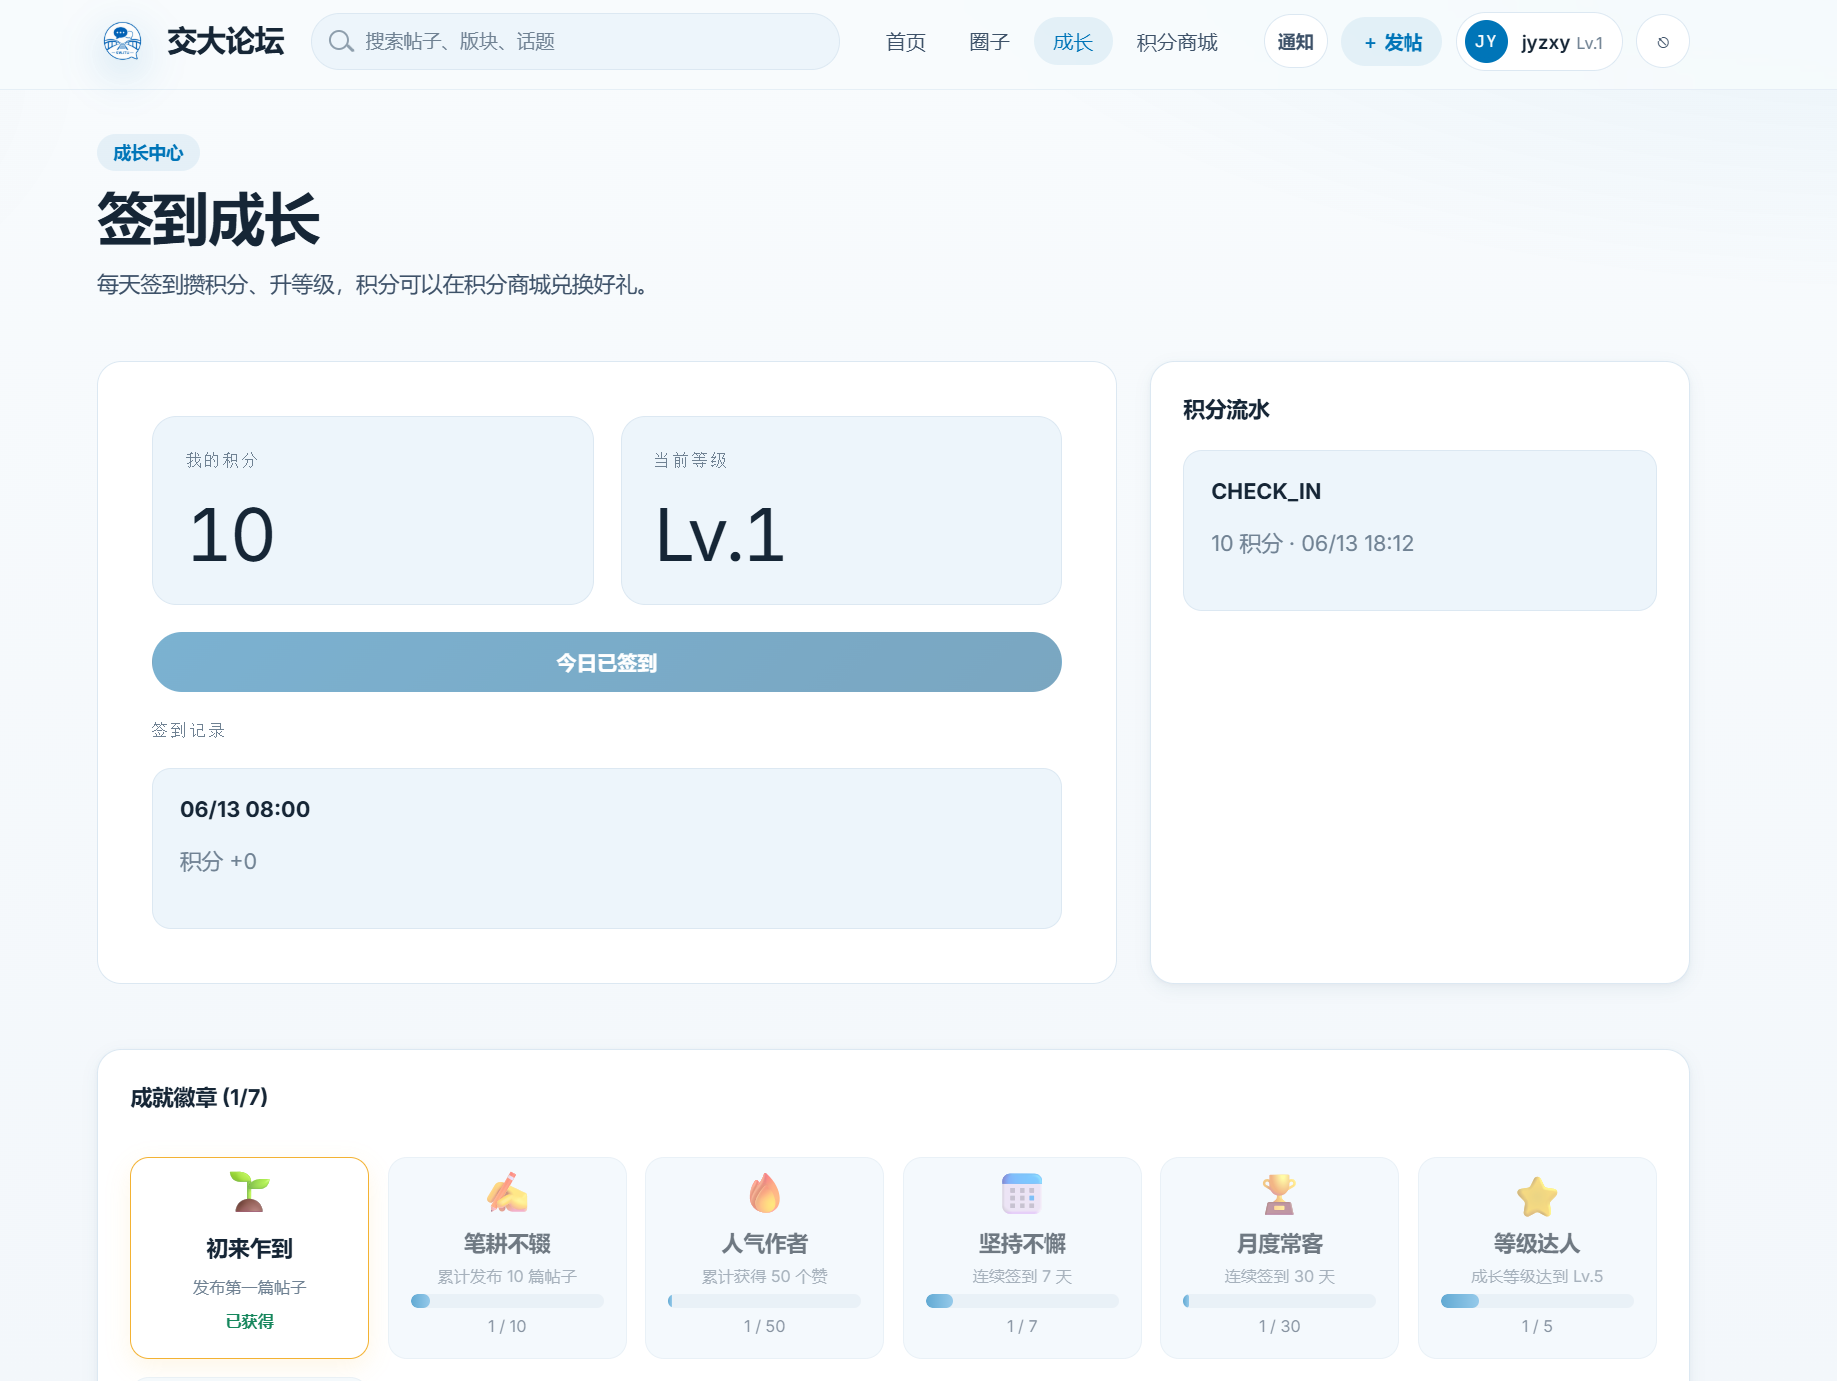
\includegraphics[width=0.85\textwidth]{figures/manual/checkin_center.png}
    \caption{成长中心签到页面}
    \label{fig:checkin-center}
\end{figure}

\subsection{积分获取方式}
积分是论坛内的虚拟货币，用于等级提升和商城兑换。获取途径包括：

\begin{table}[!htbp]
    \caption{积分获取途径与规则}
    \label{tab:points-rules}
    \centering
    \small
    \begin{tabular}{p{0.25\textwidth}p{0.20\textwidth}p{0.35\textwidth}}
        \toprule[1.5pt]
        获取方式 & 积分数量 & 说明与限制 \\
        \midrule[1pt]
        每日签到 & 10 积分 & 每日一次，同时获得 5 经验值 \\
        发布帖子 & 10--30 积分 & 审核通过后发放，精华帖额外 20 分 \\
        发表评论 & 2--5 积分 & 每条评论 2 分，被点赞超 10 次额外 3 分 \\
        收藏帖子 & 1 积分 & 每日上限 10 分 \\
        被点赞 & 1 积分 & 每次被点赞获得 1 分，每日上限 20 分 \\
        完善资料 & 50 积分 & 首次完成头像、学院、专业填写 \\
        校园认证 & 100 积分 & 首次完成校园身份认证 \\
        \bottomrule[1.5pt]
    \end{tabular}
\end{table}

积分变动记录可在「个人中心 $\rightarrow$ 积分明细」查看，包含时间、类型、数量和余额。具体奖励发放以系统当前规则为准。



\begin{figure}[!htbp]
    \centering
    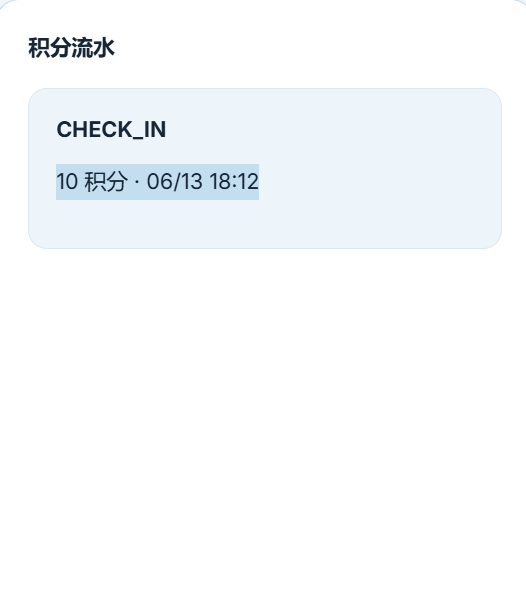
\includegraphics[width=0.85\textwidth]{figures/manual/points_history.png}
    \caption{积分明细页面}
    \label{fig:points-history}
\end{figure}

\subsection{积分商城}
进入「积分商城」页面，浏览可兑换奖品列表。奖品有校园咖啡兑换券，图书馆自习室优先券。（后续可动态添加）兑换流程：

\begin{enumerate}[leftmargin=2em]
    \item 选择奖品，查看详情页的积分价格、库存数量和兑换说明
    \item 点击「申请兑换」，确认收货地址（实物奖品）或选择账号（虚拟奖品）
    \item 提交兑换申请，积分实时扣除，申请进入「待处理」状态
    \item 管理员审核通过后，虚拟奖品即时发放，实物奖品进入发货流程
    \item 在「我的兑换」页面查看处理进度，实物奖品可查看物流信息
\end{enumerate}



\begin{figure}[!htbp]
    \centering
    \begin{subfigure}{0.48\textwidth}
        \centering
        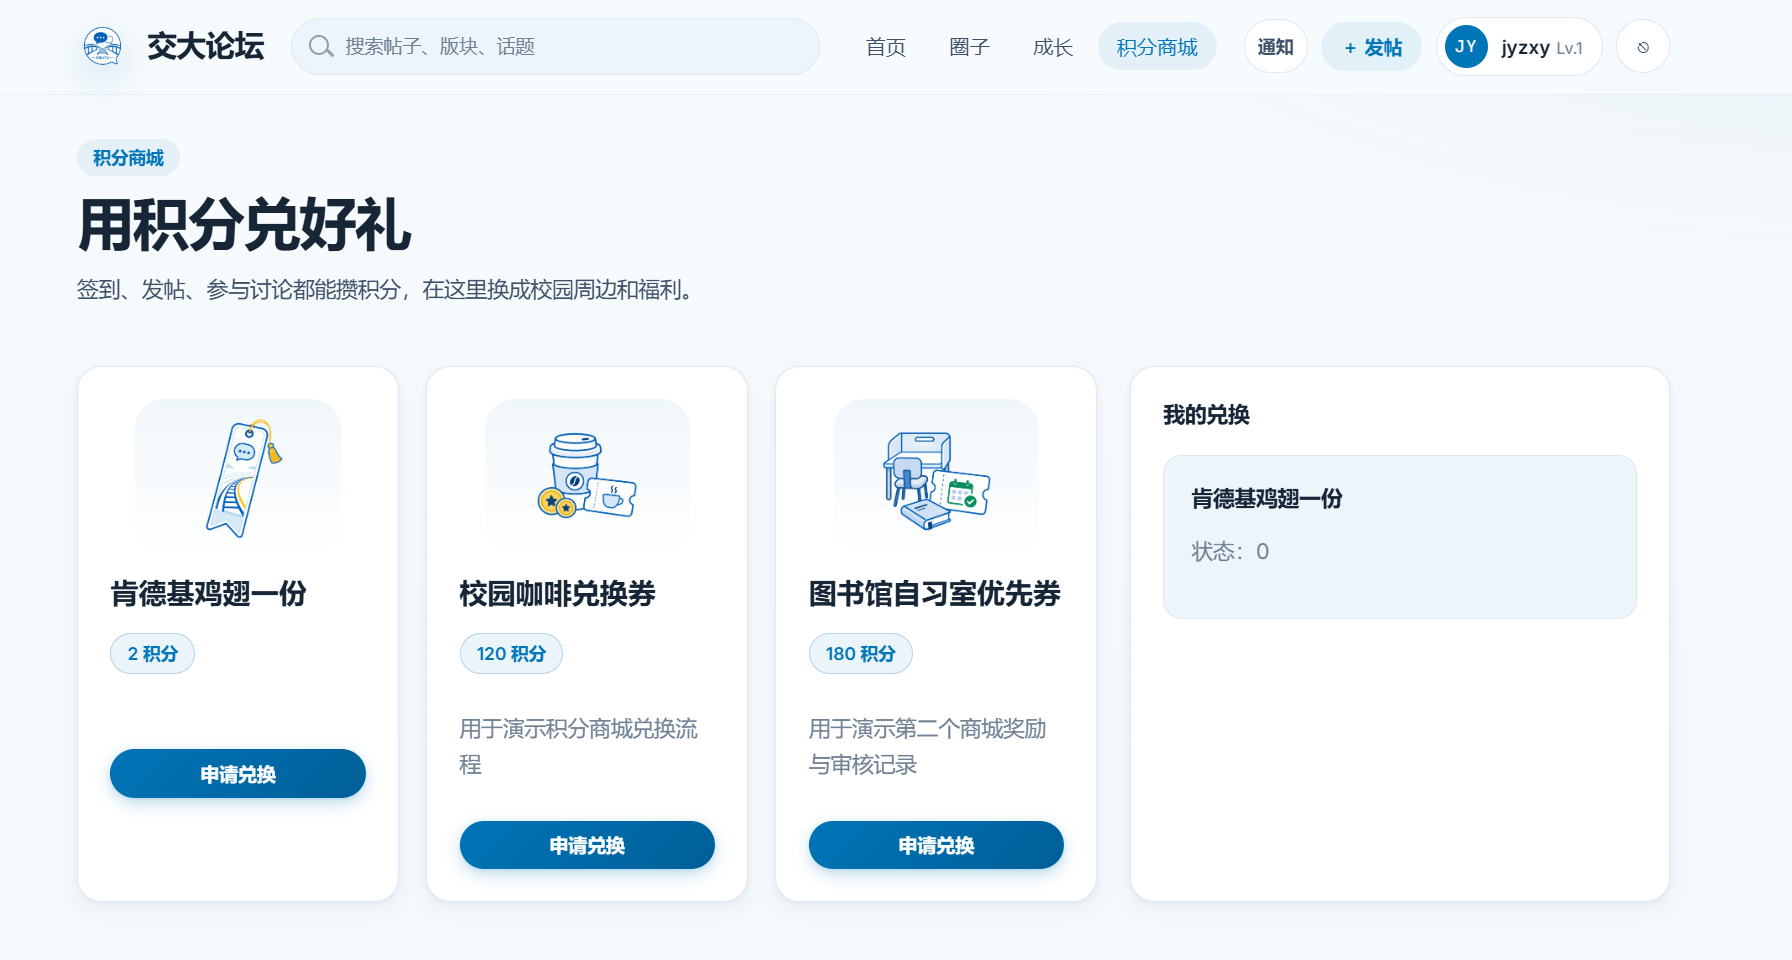
\includegraphics[width=\textwidth]{figures/manual/points_mall.png}
        \caption{积分商城首页}
    \end{subfigure}
    \hfill
    \begin{subfigure}{0.48\textwidth}
        \centering
        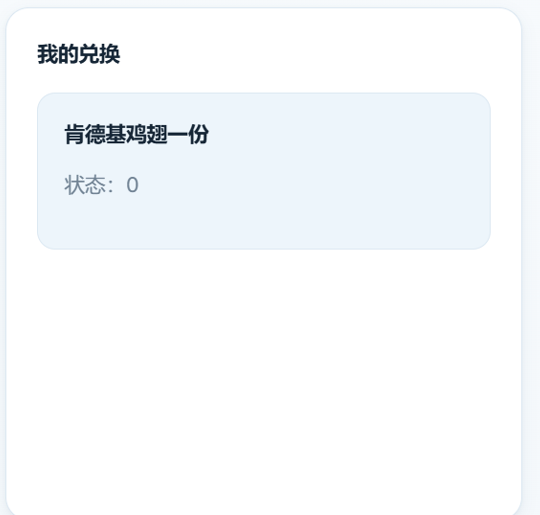
\includegraphics[width=\textwidth]{figures/manual/my_exchanges.png}
        \caption{我的兑换记录}
    \end{subfigure}
    \caption{积分商城与兑换功能}
    \label{fig:points-mall}
\end{figure}

\subsection{等级成长}
随着积分积累，用户等级自动提升。等级体系如下：


\section{个人中心}

\subsection{编辑资料}
进入「个人中心 $\rightarrow$ 编辑资料」页面，可修改以下信息：

\begin{itemize}[leftmargin=2em]
    \item \textbf{头像}：支持本地上传（JPG/PNG，最大 5MB）和裁剪，预览后保存
    \item \textbf{个人简介}：最多 200 字，支持表情符号，展示于个人主页
    \item \textbf{学院/专业}：下拉选择，与校园认证信息联动
\end{itemize}


\begin{figure}[!htbp]
    \centering
    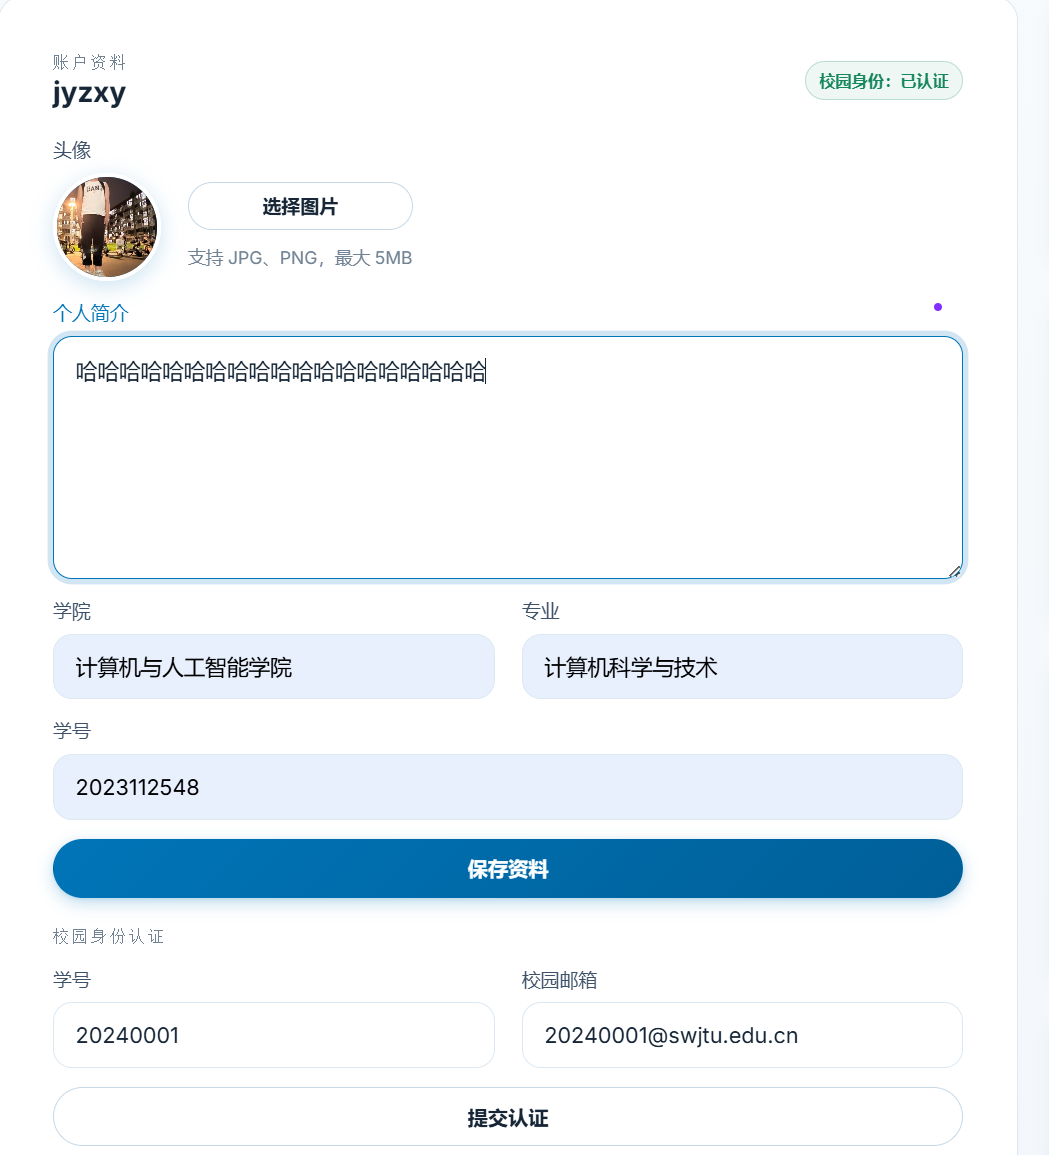
\includegraphics[width=0.85\textwidth]{figures/manual/edit_profile.png}
    \caption{个人资料编辑页面}
    \label{fig:edit-profile}
\end{figure}

\subsection{我的帖子}
「个人中心 $\rightarrow$ 我的帖子」展示用户发布的所有帖子，支持以下操作：

\begin{itemize}[leftmargin=2em]
    \item \textbf{状态筛选}：全部/已发布/已隐藏
    \item \textbf{编辑帖子}：未审核或已发布的帖子可修改标题、内容和标签
    \item \textbf{撤回帖子}：已发布帖子可撤回至草稿状态，撤回后不在首页展示
    \item \textbf{删除帖子}：永久删除帖子及关联评论，积分不扣除但不可恢复
    \item \textbf{数据展示}：每帖展示浏览量、点赞数、评论数、收藏数和发布时间
\end{itemize}

=

\begin{figure}[!htbp]
    \centering
    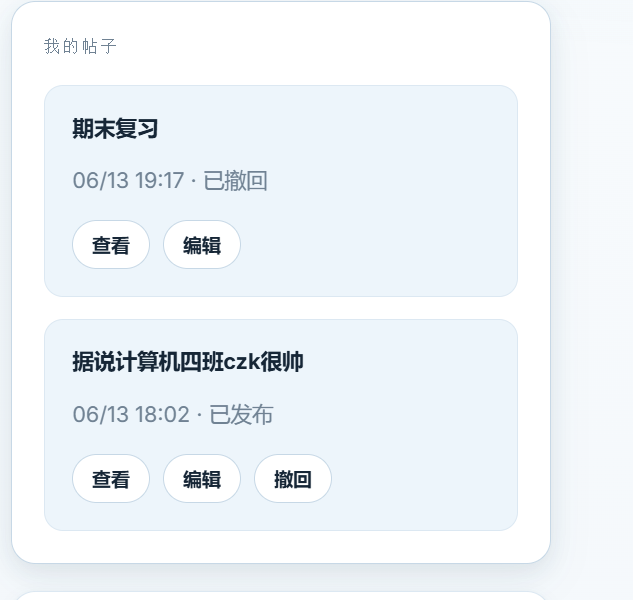
\includegraphics[width=0.48\textwidth]{figures/manual/my_posts1.png}
    \caption{我的帖子管理页面}
    \label{fig:my-posts}
\end{figure}
\begin{figure}[!htbp]
	\centering
	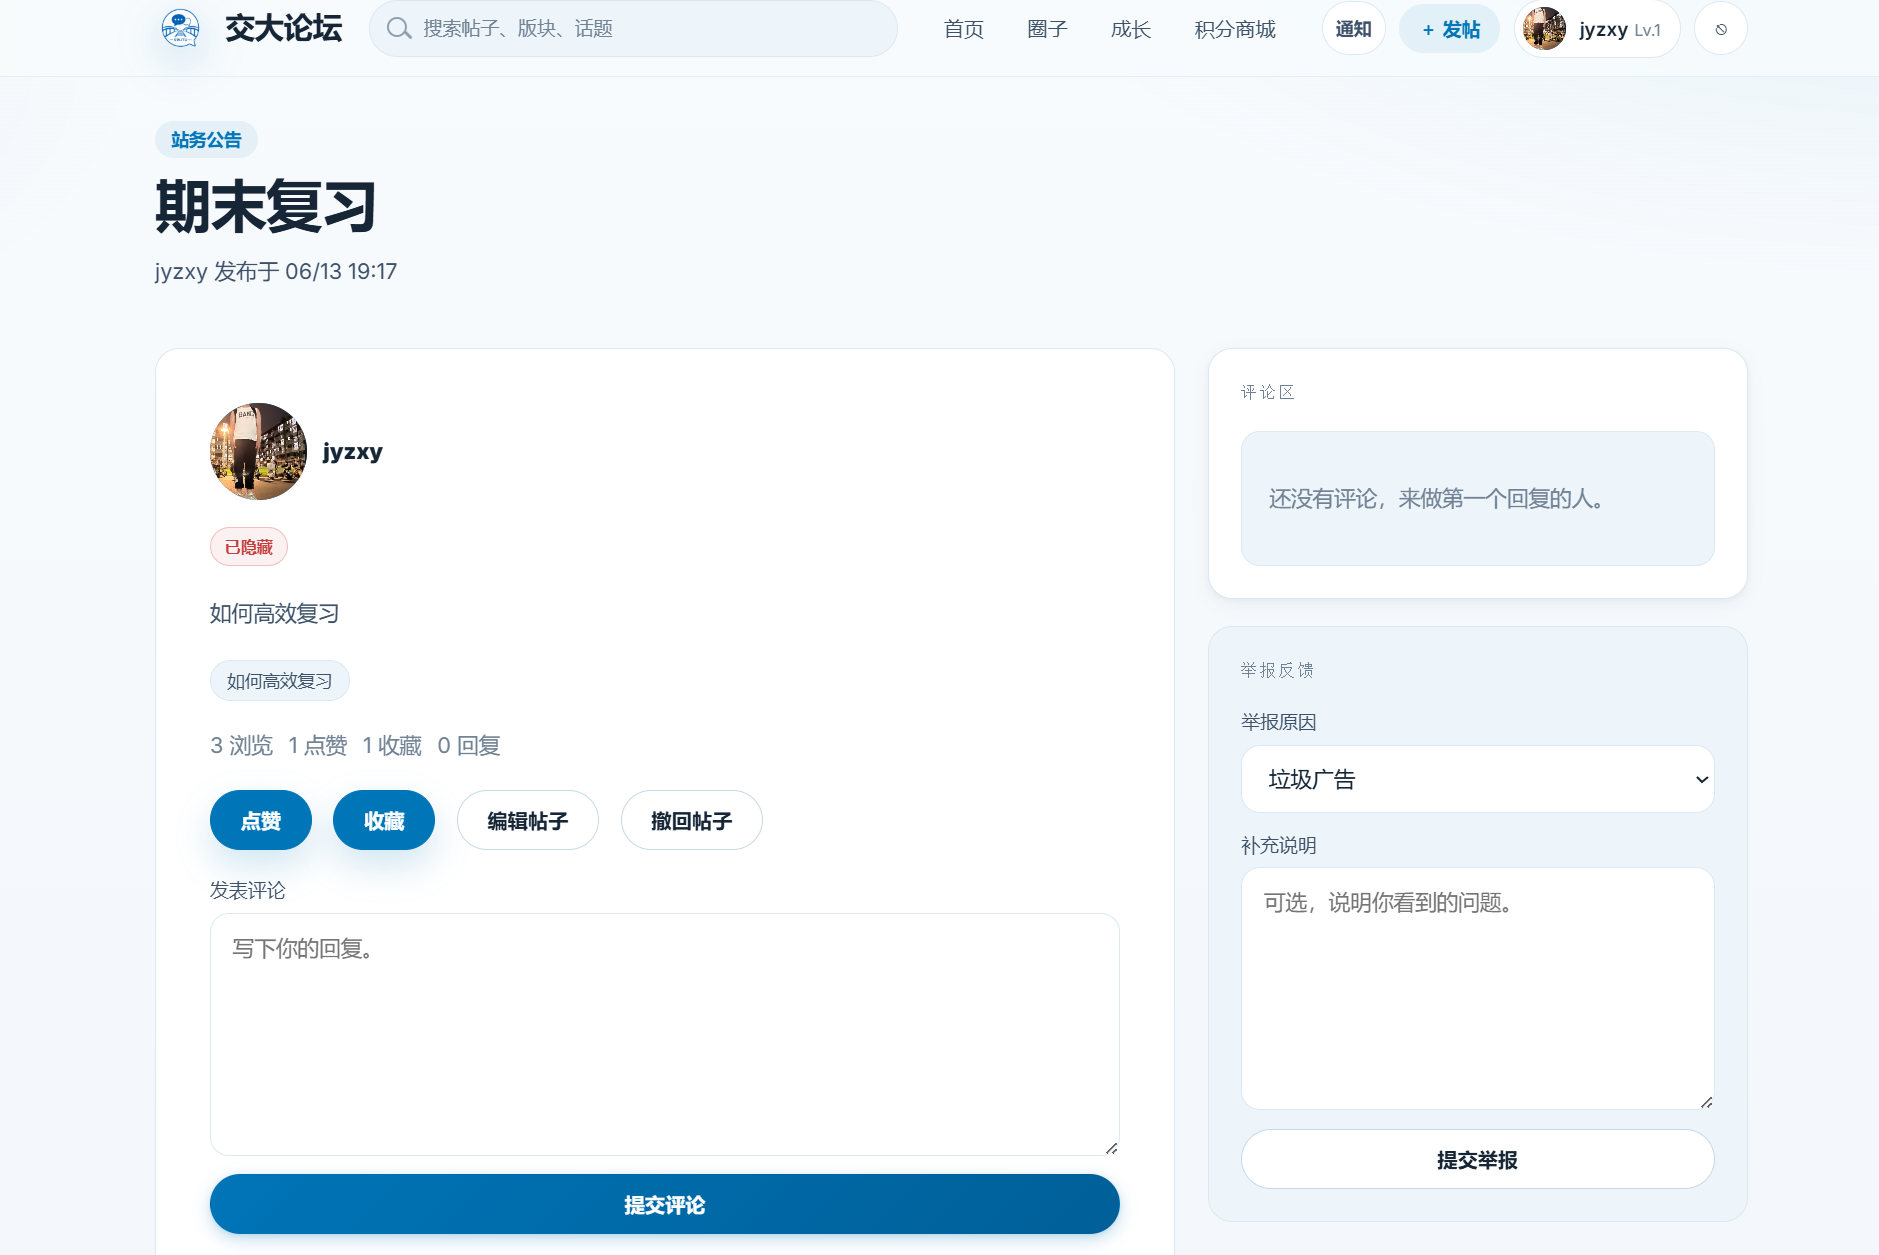
\includegraphics[width=0.48\textwidth]{figures/manual/my_posts2.png}
	\caption{我的帖子管理页面}
	\label{fig:my-posts-list}
\end{figure}

\subsection{我的收藏与浏览记录}
「我的收藏」页面展示用户收藏的所有帖子，支持按收藏时间排序、按版块筛选和取消收藏。「浏览记录」页面展示最近浏览历史，支持清空记录和按日期筛选。两个页面均采用与首页一致的卡片布局，确保视觉统一。


\begin{figure}[!htbp]
    \centering
    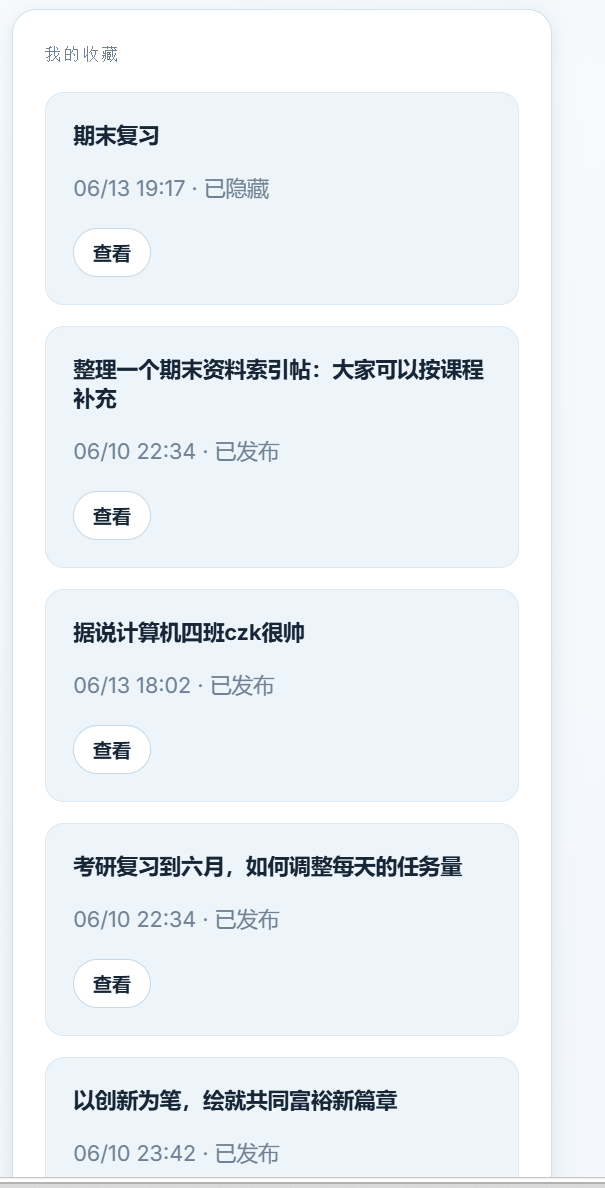
\includegraphics[width=0.48\textwidth]{figures/manual/my_collections_full.png}
    \caption{我的收藏完整页面}
    \label{fig:my-collections-full}
\end{figure}
\begin{figure}[!htbp]
	\centering
	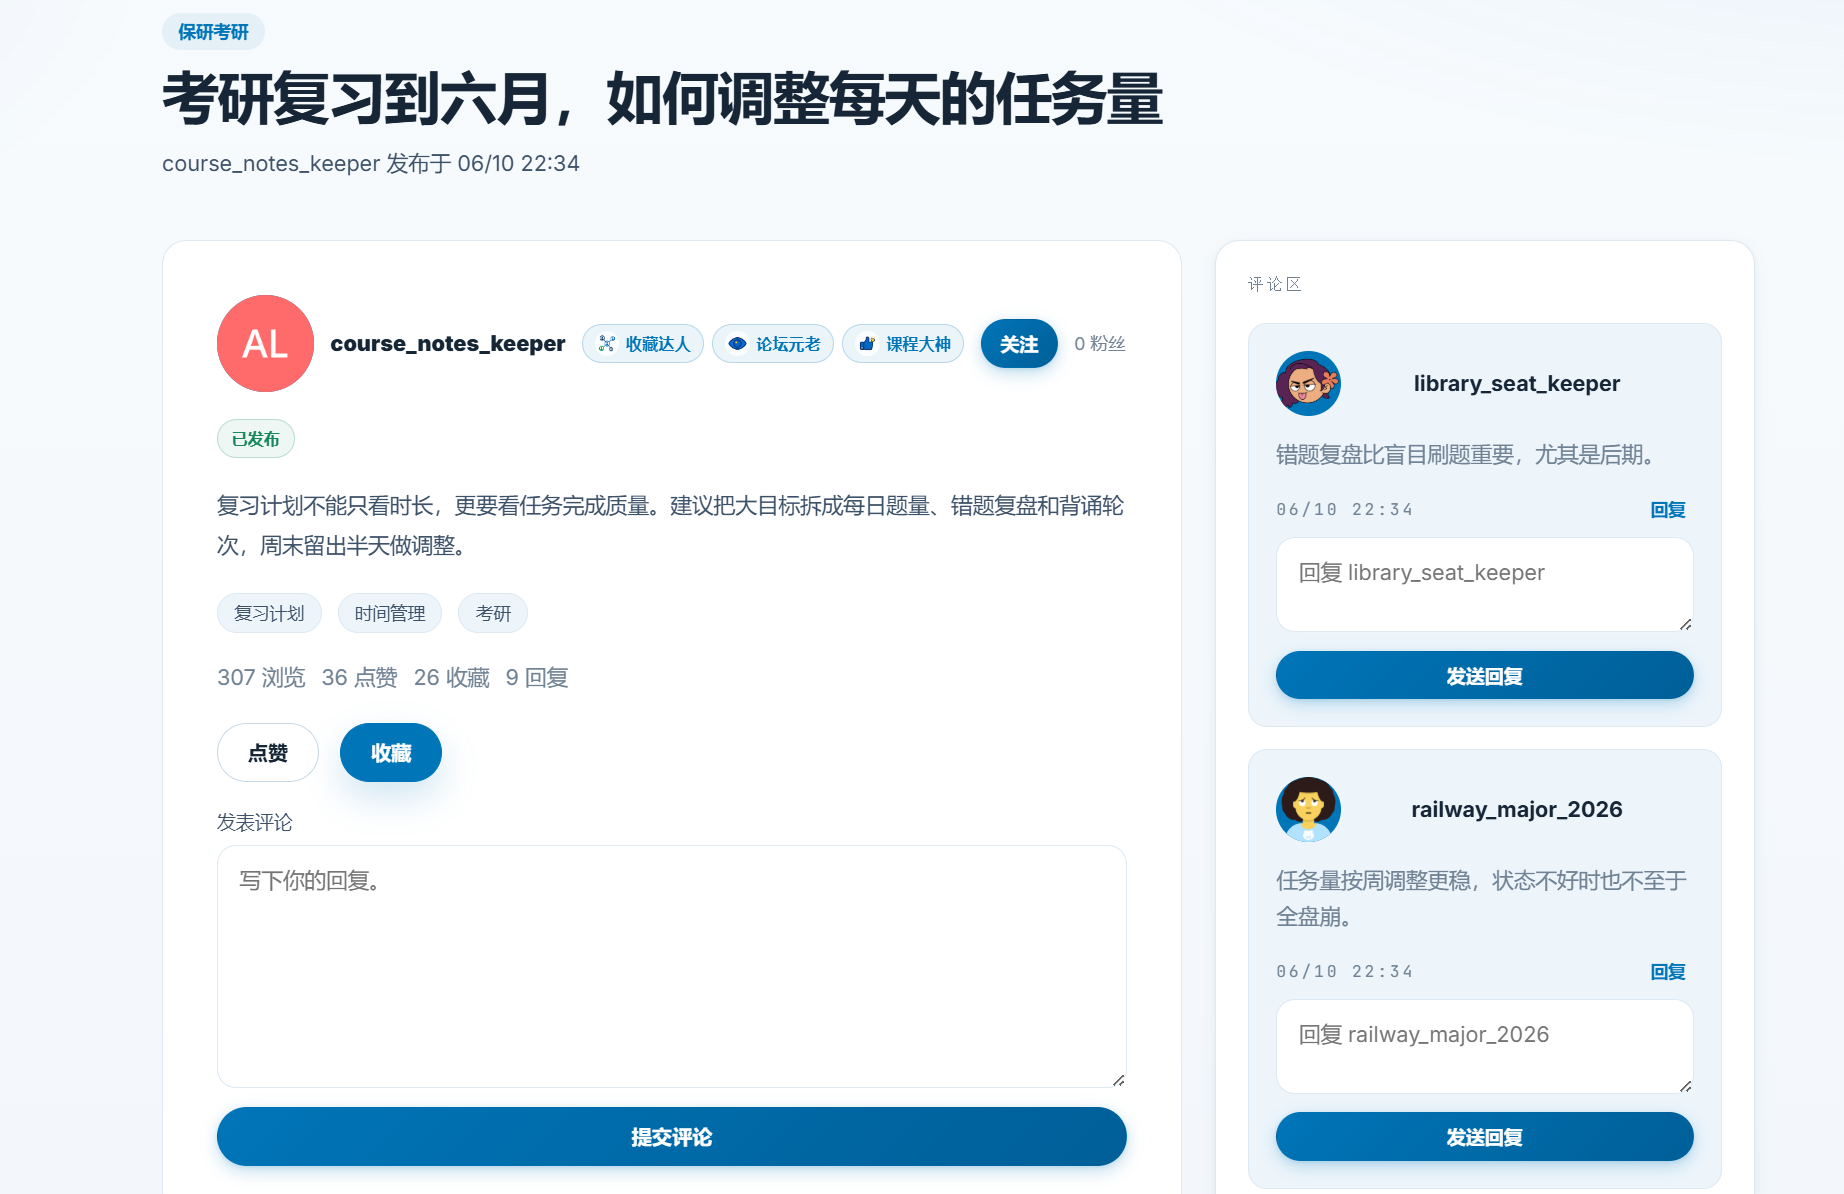
\includegraphics[width=0.48\textwidth]{figures/manual/my_collections_full1.png}
	\caption{查看收藏帖子的详细内容}
	\label{fig:my-collections-list}
\end{figure}
\section{通知中心}

\subsection{通知类型}
页面右上角「通知」按钮（铃铛图标）显示未读通知数量红点。点击后展开通知下拉面板，展示最近 10 条通知。通知类型包括：

\begin{itemize}[leftmargin=2em]
    \item \textbf{帖子审核结果}：帖子通过审核/被驳回/被隐藏，附带帖子标题和原因
    \item \textbf{评论回复提醒}：其他用户回复了你的评论，附带评论摘要和跳转链接
    \item \textbf{点赞提醒}：帖子或评论获得新点赞，合并展示（「张三等 5 人赞了你的帖子」）
    \item \textbf{关注提醒}：有新用户关注了你，附带用户头像和昵称
    \item \textbf{等级提升通知}：积分达到升级标准，展示新等级和解锁权益
    \item \textbf{兑换申请处理}：积分商城兑换申请被通过/驳回，附带奖品名称和处理备注
    \item \textbf{系统公告}：论坛维护通知、活动推送、规则更新等
\end{itemize}



\begin{figure}[!htbp]
    \centering
    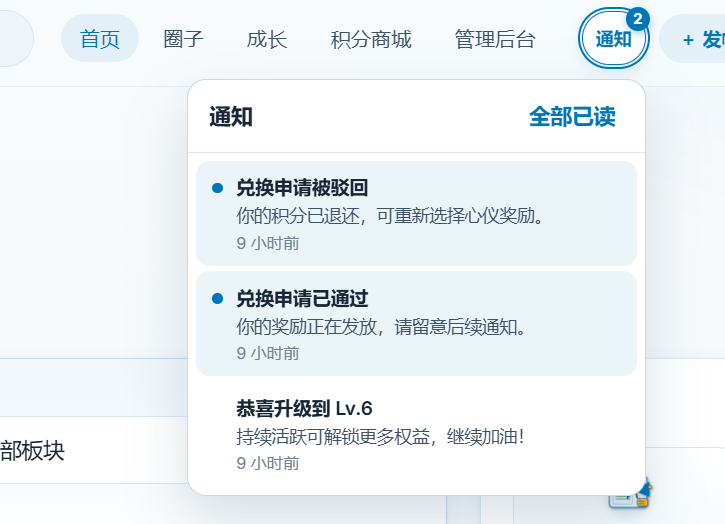
\includegraphics[width=0.55\textwidth]{figures/manual/notification_panel.png}
    \caption{通知中心下拉面板}
    \label{fig:notification-panel}
\end{figure}

\subsection{通知管理}


\begin{itemize}[leftmargin=2em]
    \item \textbf{全部已读}：一键标记所有通知为已读状态，清除红点提醒
    \item \textbf{删除通知}：单条删除或批量删除已读通知

\end{itemize}



\begin{figure}[!htbp]
    \centering
    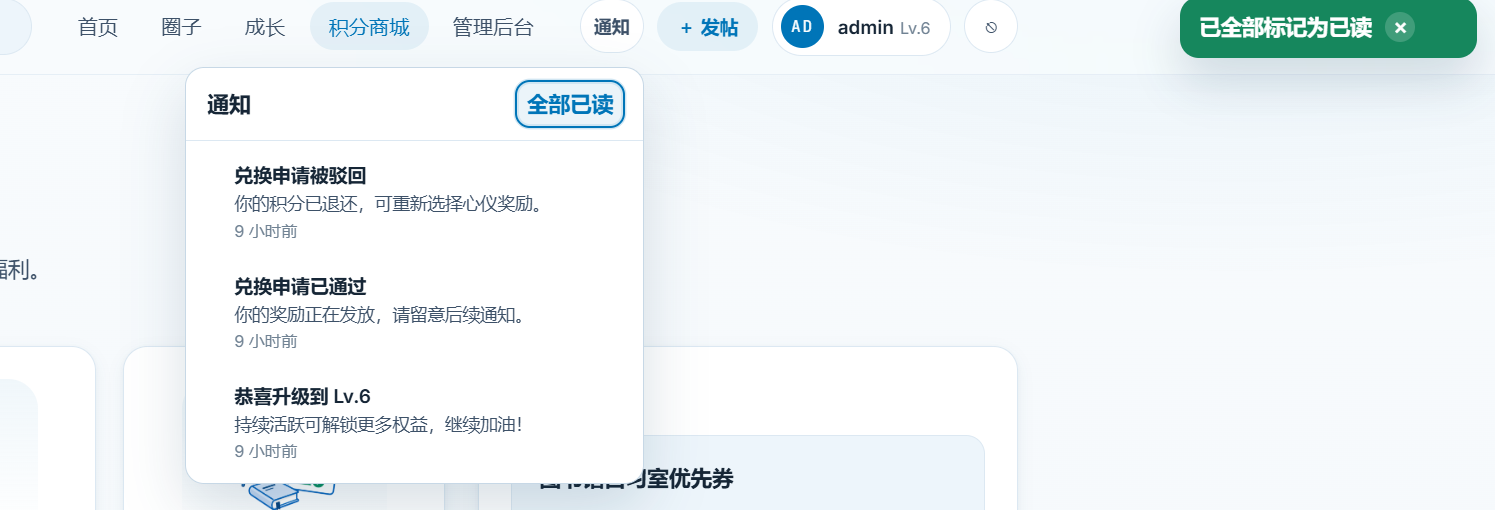
\includegraphics[width=0.92\textwidth]{figures/manual/notification_detail.png}
    \caption{通知详情页面}
    \label{fig:notification-detail}
\end{figure}

\section{关注与社交}

\subsection{关注用户}
在帖子详情页点击作者头像进入用户主页，或点击评论区的用户昵称，均可查看用户资料并点击「关注」按钮。关注后：

\begin{itemize}[leftmargin=2em]
    \item 该用户发布的新帖将在你的首页「关注动态」流中优先展示
    \item 该用户的个人主页显示「已关注」状态，可点击取消关注
    \item 互相关注后，双方可在个人资料页查看对方的联系方式（若已设置）
    \item 关注列表可在「个人中心 $\rightarrow$ 我的关注」查看，支持按关注时间排序和搜索
\end{itemize}



\begin{figure}[!htbp]
    \centering
    \begin{subfigure}{0.48\textwidth}
        \centering
        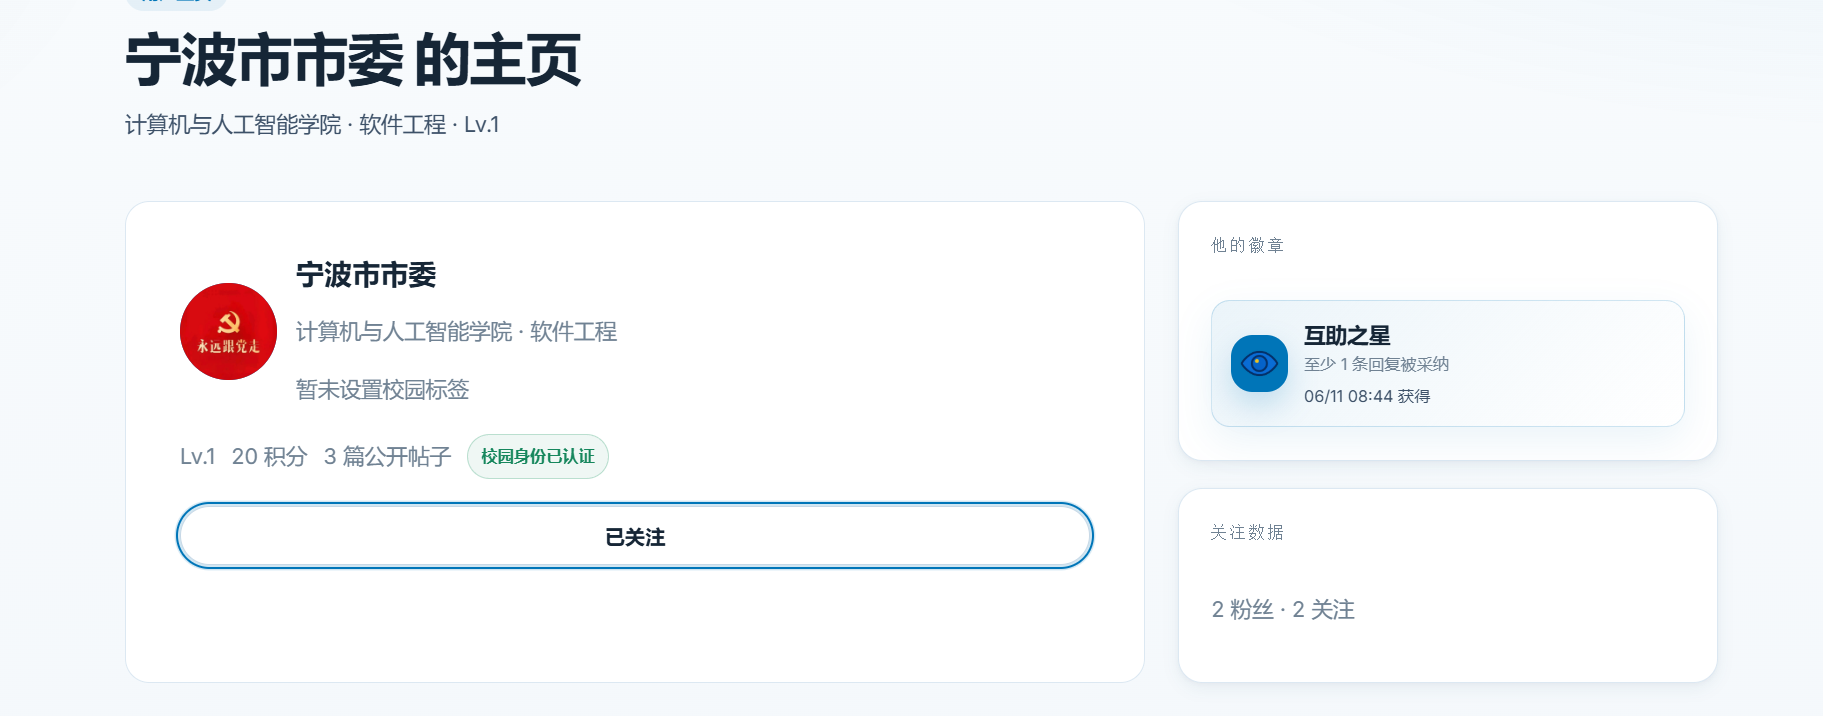
\includegraphics[width=\textwidth]{figures/manual/user_profile_follow.png}
        \caption{用户主页与关注按钮}
    \end{subfigure}
    \hfill
    \begin{subfigure}{0.48\textwidth}
        \centering
        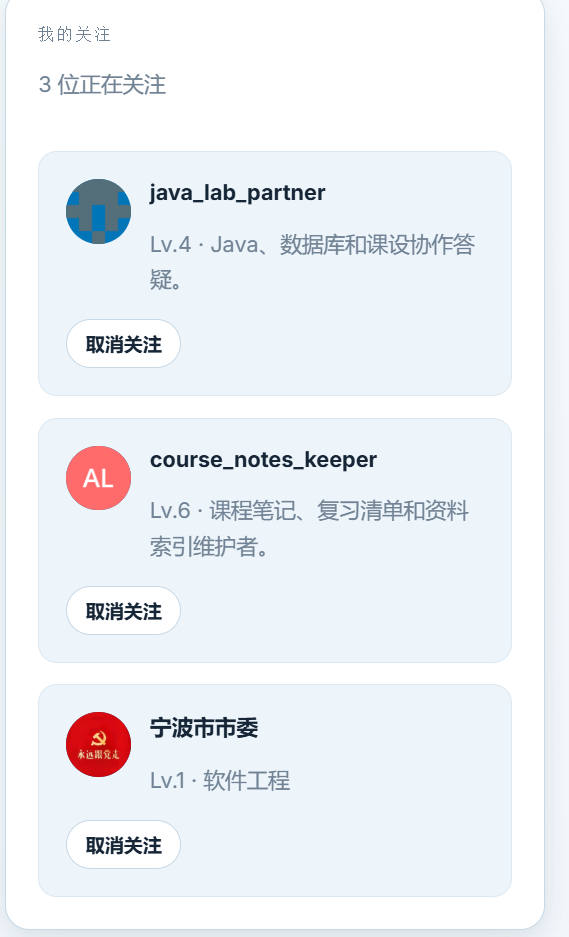
\includegraphics[width=\textwidth]{figures/manual/my_following.png}
        \caption{我的关注列表}
    \end{subfigure}
    \caption{关注与社交功能}
    \label{fig:social-features}
\end{figure}

\subsection{个人主页}
每个用户拥有独立的个人主页，URL 格式为 \url{https://forum.swjtu.edu.cn/user/{username}}。主页展示内容：

\begin{itemize}[leftmargin=2em]
    \item 头像、昵称、等级徽章、认证标识、关注数/粉丝数/获赞数统计
    \item 个人简介、学院专业信息（若公开）
    \item 最近发布的帖子列表（最多 10 条）
    \item 最近获得的点赞和评论动态
    \item 加入时间、最后活跃时间
\end{itemize}

访客视角下，根据被访用户的隐私设置，部分信息可能隐藏。用户可自定义主页背景图（高等级权益）。



\begin{figure}[!htbp]
    \centering
    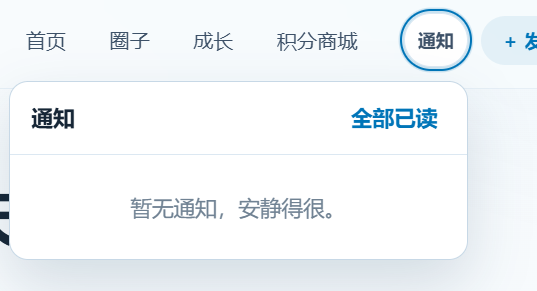
\includegraphics[width=0.92\textwidth]{figures/manual/user_profile_full.png}
    \caption{用户个人主页完整界面}
    \label{fig:user-profile-full}
\end{figure}

\section{管理后台（仅管理员）}

\subsection{管理员入口}
管理员用户登录后，顶部导航栏右侧新增「管理后台」入口）。点击后进入独立的管理后台界面。



\begin{figure}[!htbp]
    \centering
    \begin{subfigure}{0.92\textwidth}
        \centering
        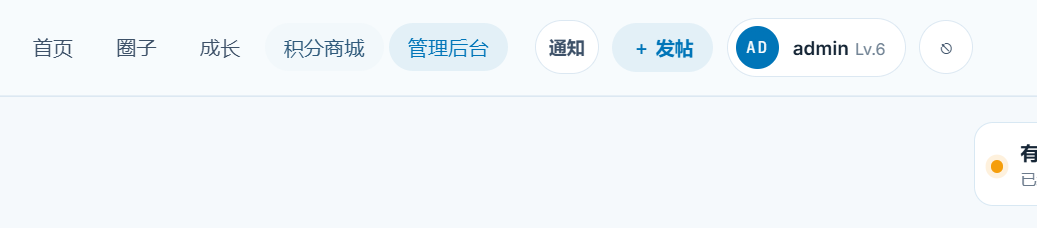
\includegraphics[width=\textwidth]{figures/manual/admin_navbar.png}
        \caption{管理员导航栏}
    \end{subfigure}

    \vspace{0.5em}

    \begin{subfigure}{0.92\textwidth}
        \centering
        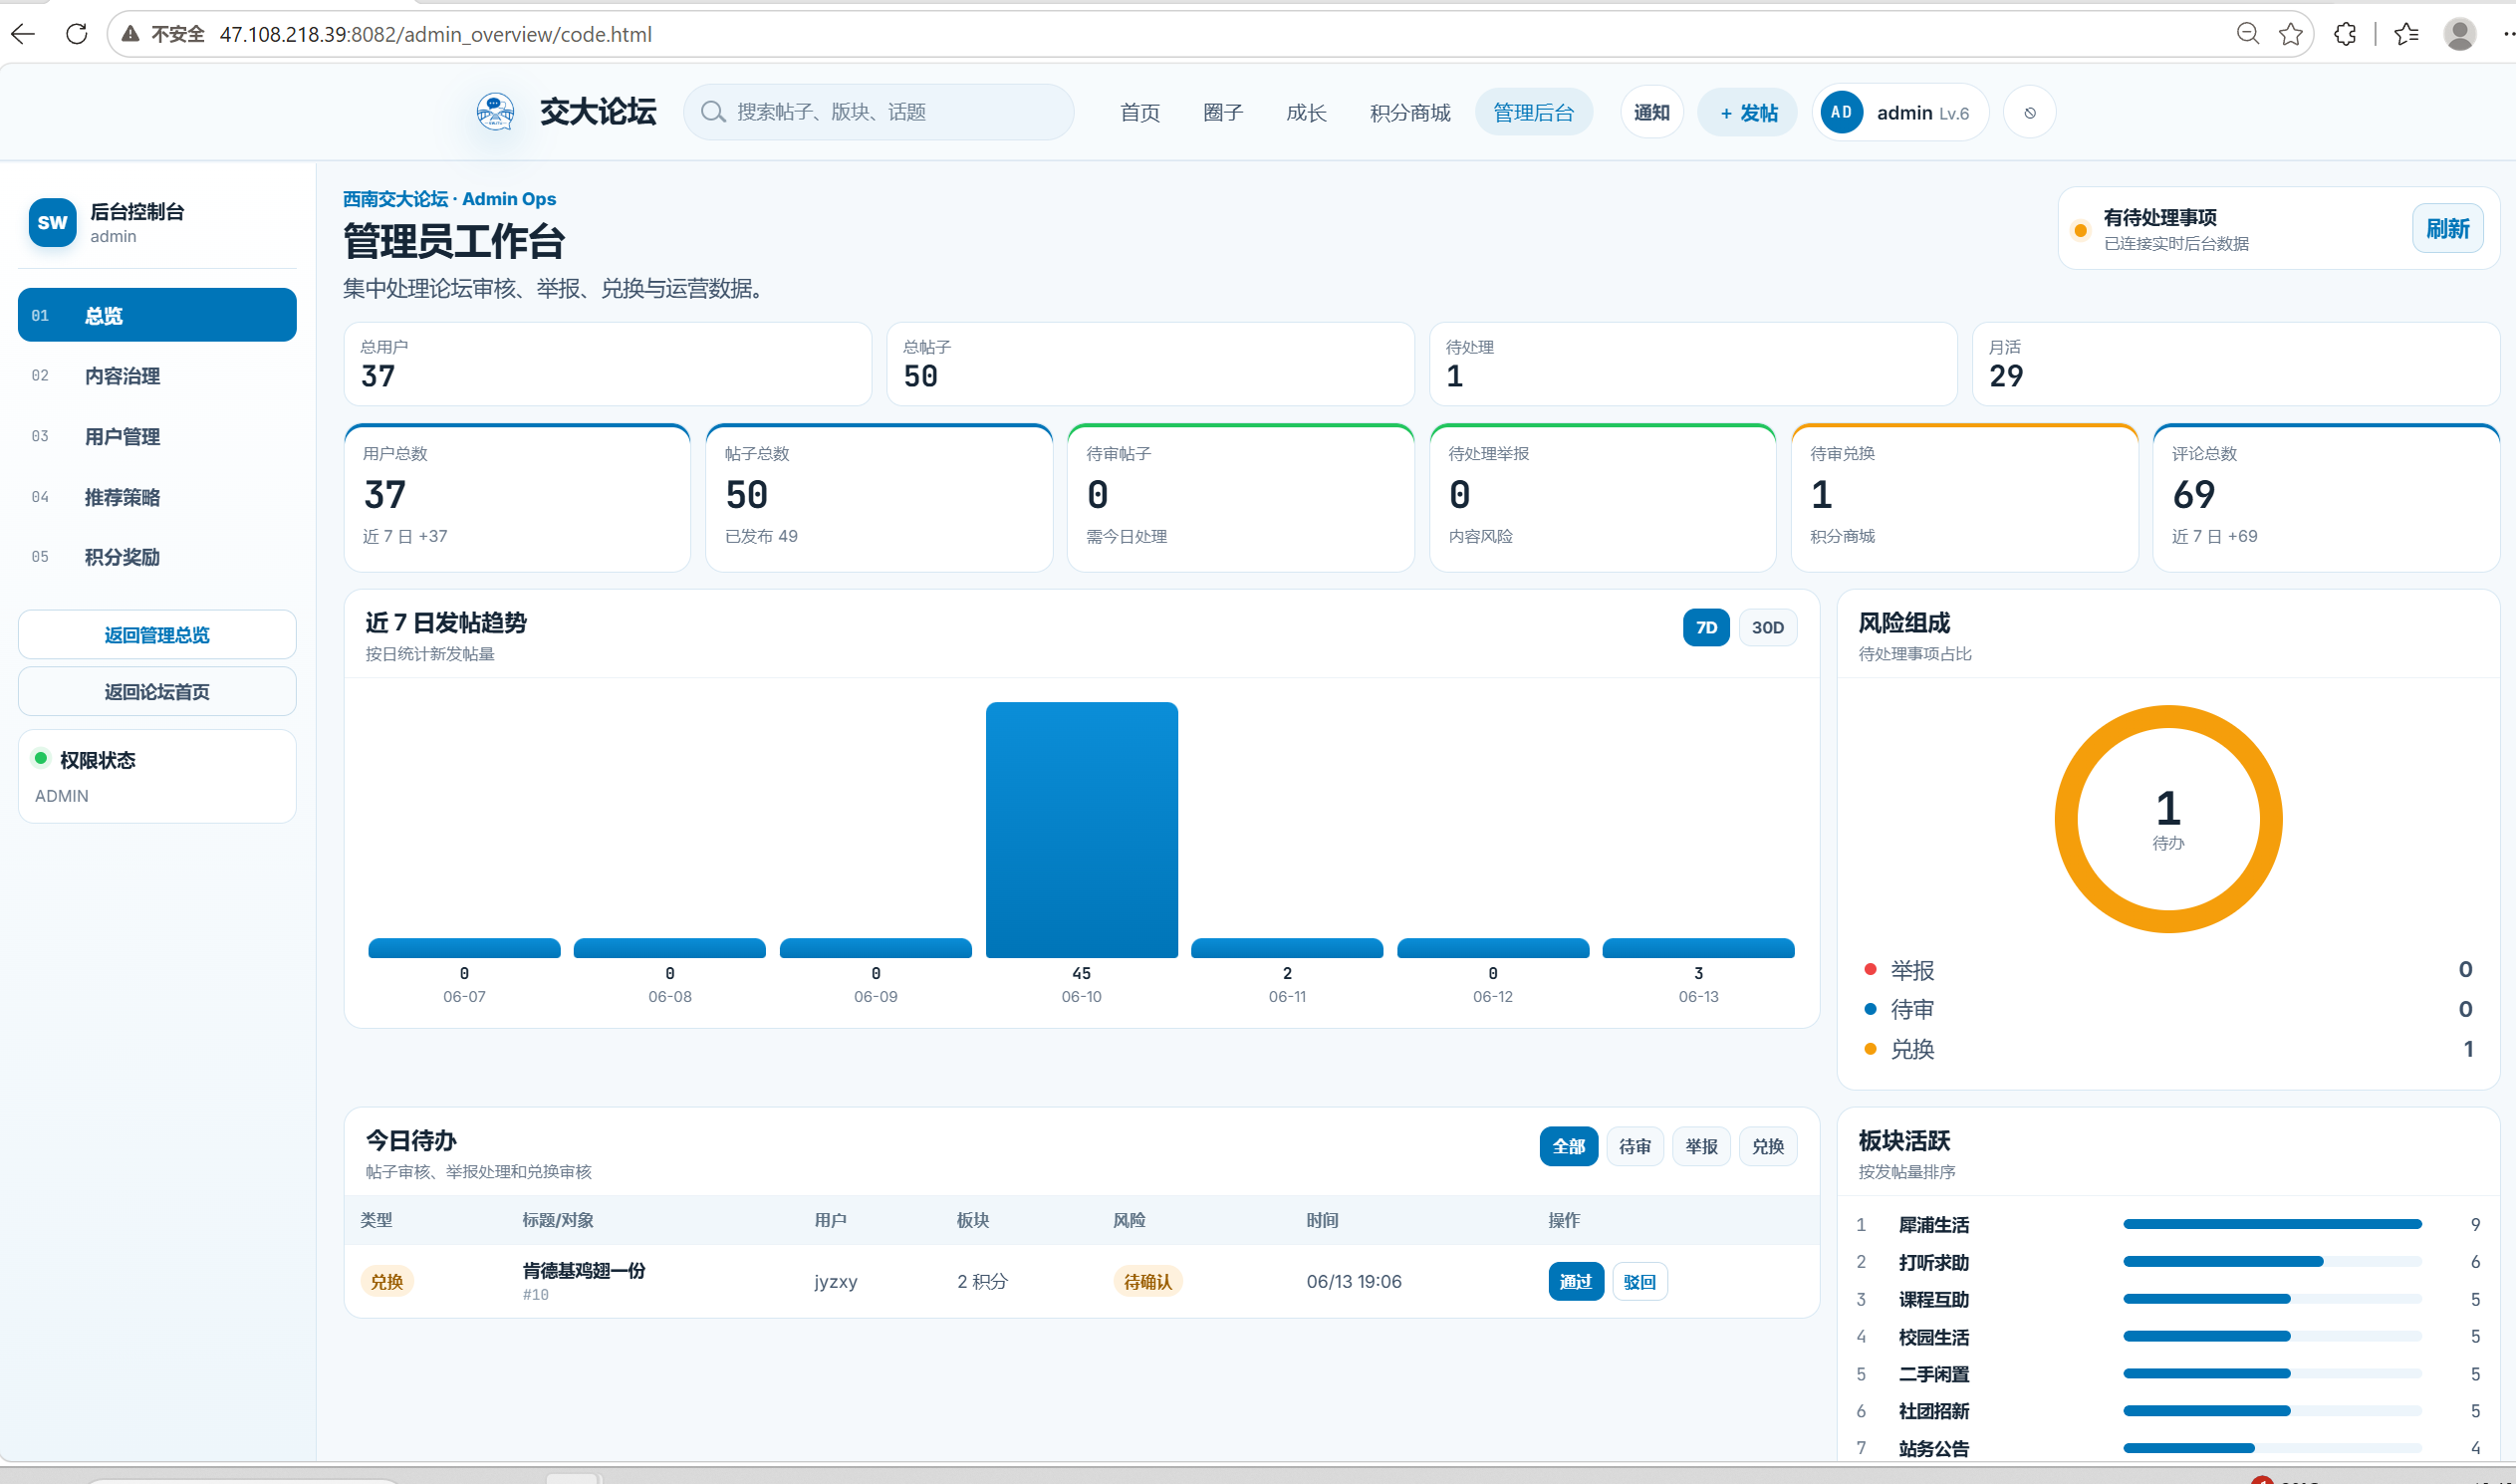
\includegraphics[width=\textwidth]{figures/manual/admin_dashboard.png}
        \caption{管理后台首页}
    \end{subfigure}
    \caption{管理员入口与后台概览}
    \label{fig:admin-entrance}
\end{figure}

\subsection{数据统计与运营报告}
管理后台首页提供论坛运营数据总览，包括以下统计卡片和图表：

\begin{itemize}[leftmargin=2em]
    \item \textbf{总览数据}：总用户数、封禁用户数、近 7 天新增用户、总帖子数、待审核帖子数、已发布帖子数、已隐藏帖子数、近 7 天新增帖子、总评论数、待处理举报数、待处理兑换申请数
    \item \textbf{发帖趋势图}：折线图展示近 7 天每日新增帖子数量，支持悬停查看具体数值
    \item \textbf{版块分布图}：饼图或柱状图展示各版块帖子数量占比
    \item \textbf{热门话题词云}：近 14 天高频标签关键词可视化展示
    \item \textbf{热门帖子排行}：表格展示热度前 5 的帖子，含浏览量、点赞数、评论数
\end{itemize}

数据支持按日、按周、按月筛选，图表支持导出为 PNG 图片。管理员可据此生成运营报告，分析论坛活跃度变化趋势。



\begin{figure}[!htbp]
    \centering
    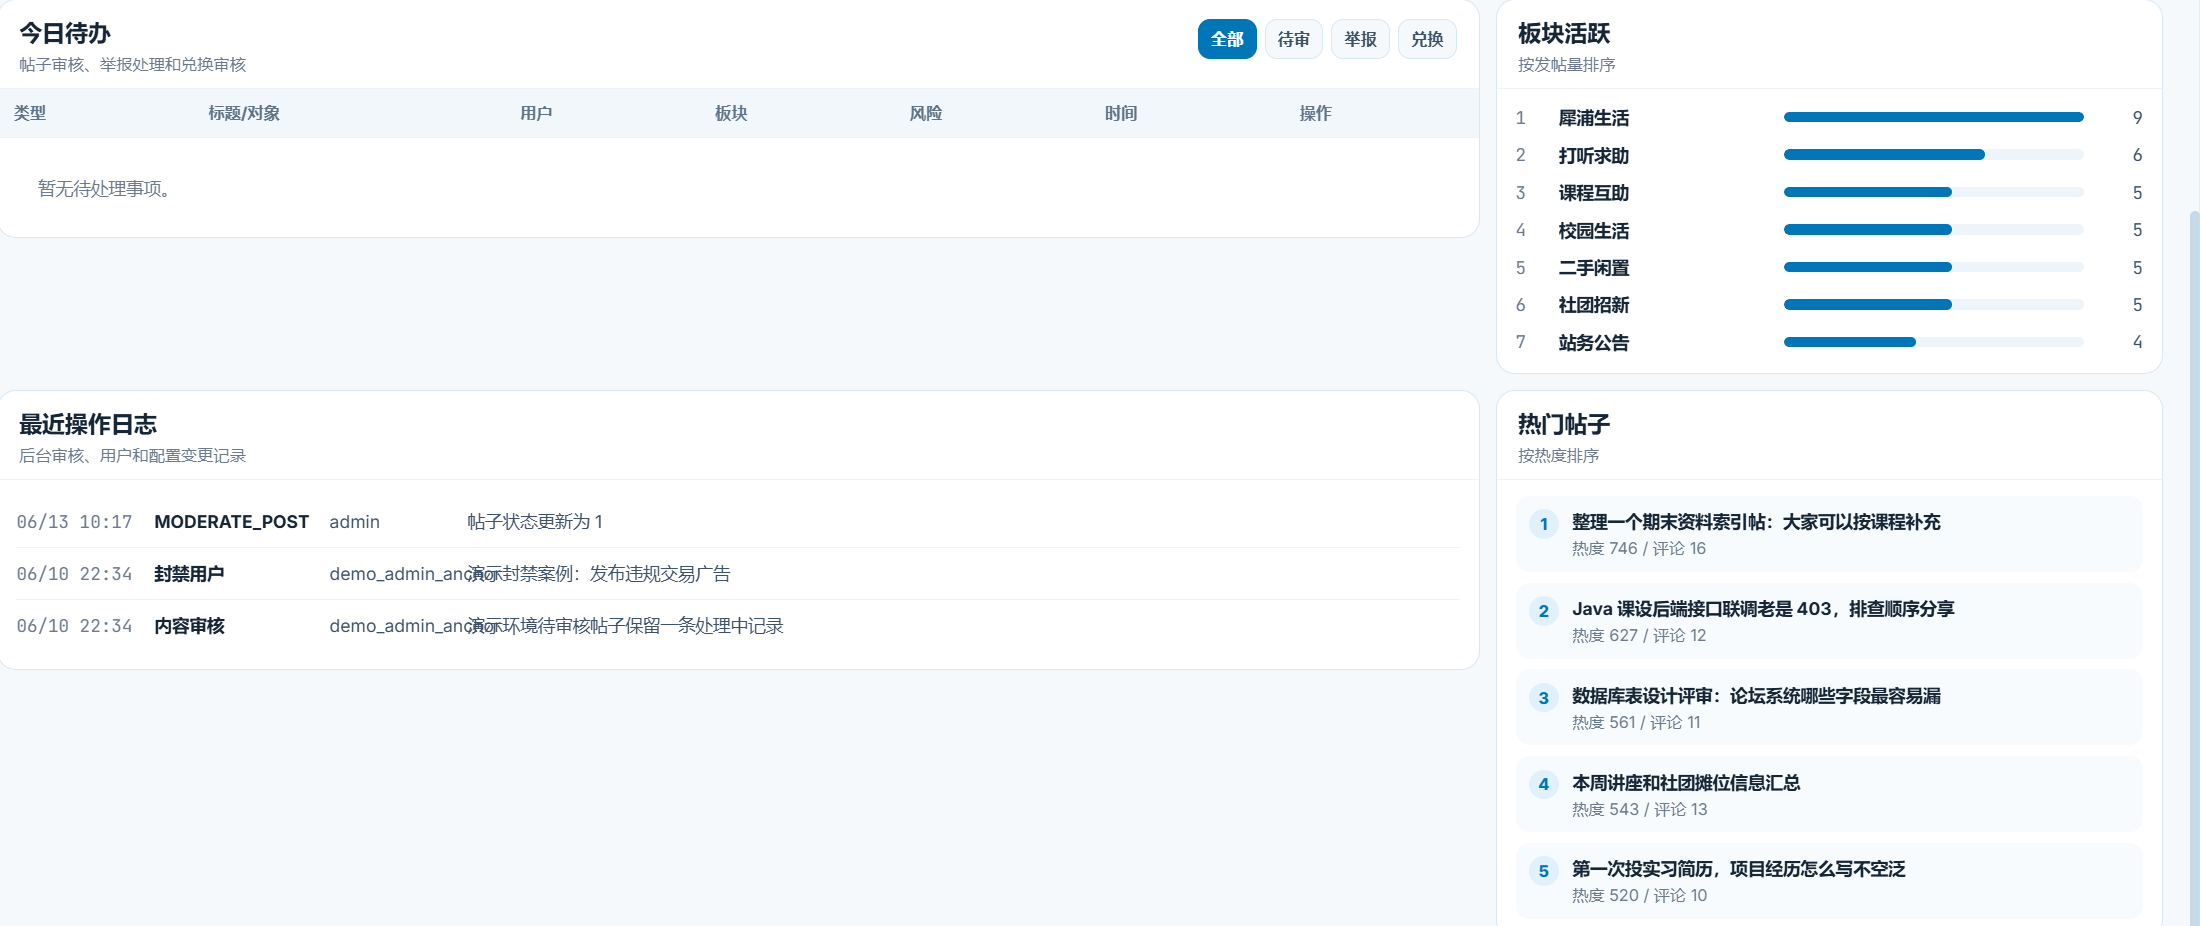
\includegraphics[width=0.48\textwidth]{figures/manual/admin_stats_dashboard.png}
    \caption{数据统计与运营报告看板1}
    \label{fig:admin-stats}
\end{figure}
\begin{figure}[!htbp]
	\centering
	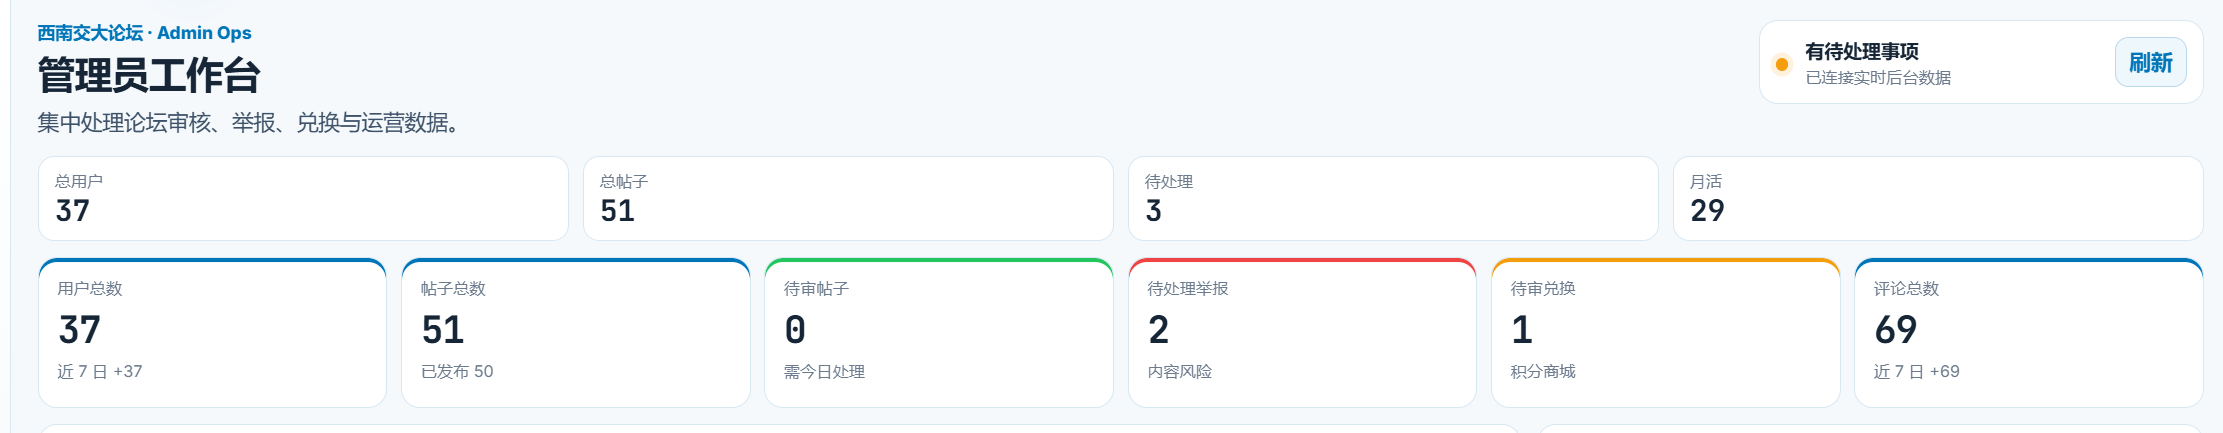
\includegraphics[width=0.48\textwidth]{figures/manual/admin_stats_dashboard1.png}
	\caption{数据统计与运营报告看板2}
	\label{fig:admin-stats-detail}
\end{figure}

\subsection{帖子审核}
「内容管理 $\rightarrow$ 帖子审核」页面展示所有待审核帖子列表，每行包含：帖子标题、作者、所属版块、提交时间、内容摘要和操作按钮。管理员可进行以下操作：

\begin{itemize}[leftmargin=2em]
    \item \textbf{通过}：帖子立即在首页和所属版块展示，作者获得积分奖励
    \item \textbf{驳回}：填写驳回原因（必填），帖子退回作者草稿箱，作者可修改后重新提交
    \item \textbf{隐藏}：已发布的帖子被隐藏，不在论坛中展示，但保留数据可恢复
    \item \textbf{批量操作}：勾选多条帖子，批量通过或批量驳回
\end{itemize}

审核页面支持按版块、提交时间、内容关键词筛选，支持分页（每页 20 条）。审核操作记录自动写入操作日志。


\begin{figure}[!htbp]
    \centering
    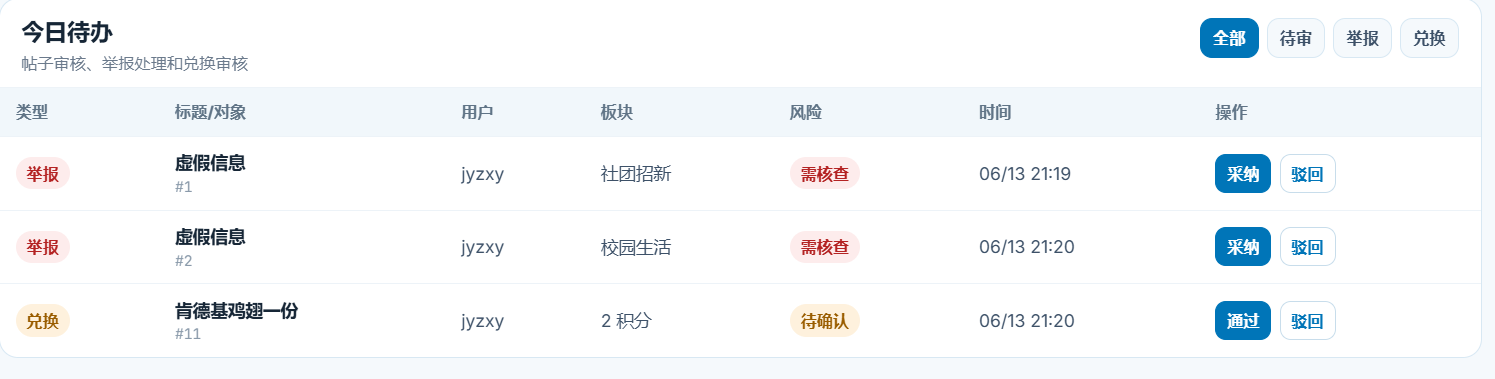
\includegraphics[width=0.92\textwidth]{figures/manual/post_audit.png}
    \caption{帖子审核管理页面}
    \label{fig:post-audit}
\end{figure}

\subsection{评论管理}
「内容管理 $\rightarrow$ 评论管理」页面展示所有评论列表，支持按帖子、用户、时间筛选。管理员可隐藏违规评论（评论变为「该评论已被隐藏」提示，不影响帖子其他评论）或恢复已隐藏评论。隐藏评论时可选填原因，并自动通知被处理用户。



\begin{figure}[!htbp]
    \centering
    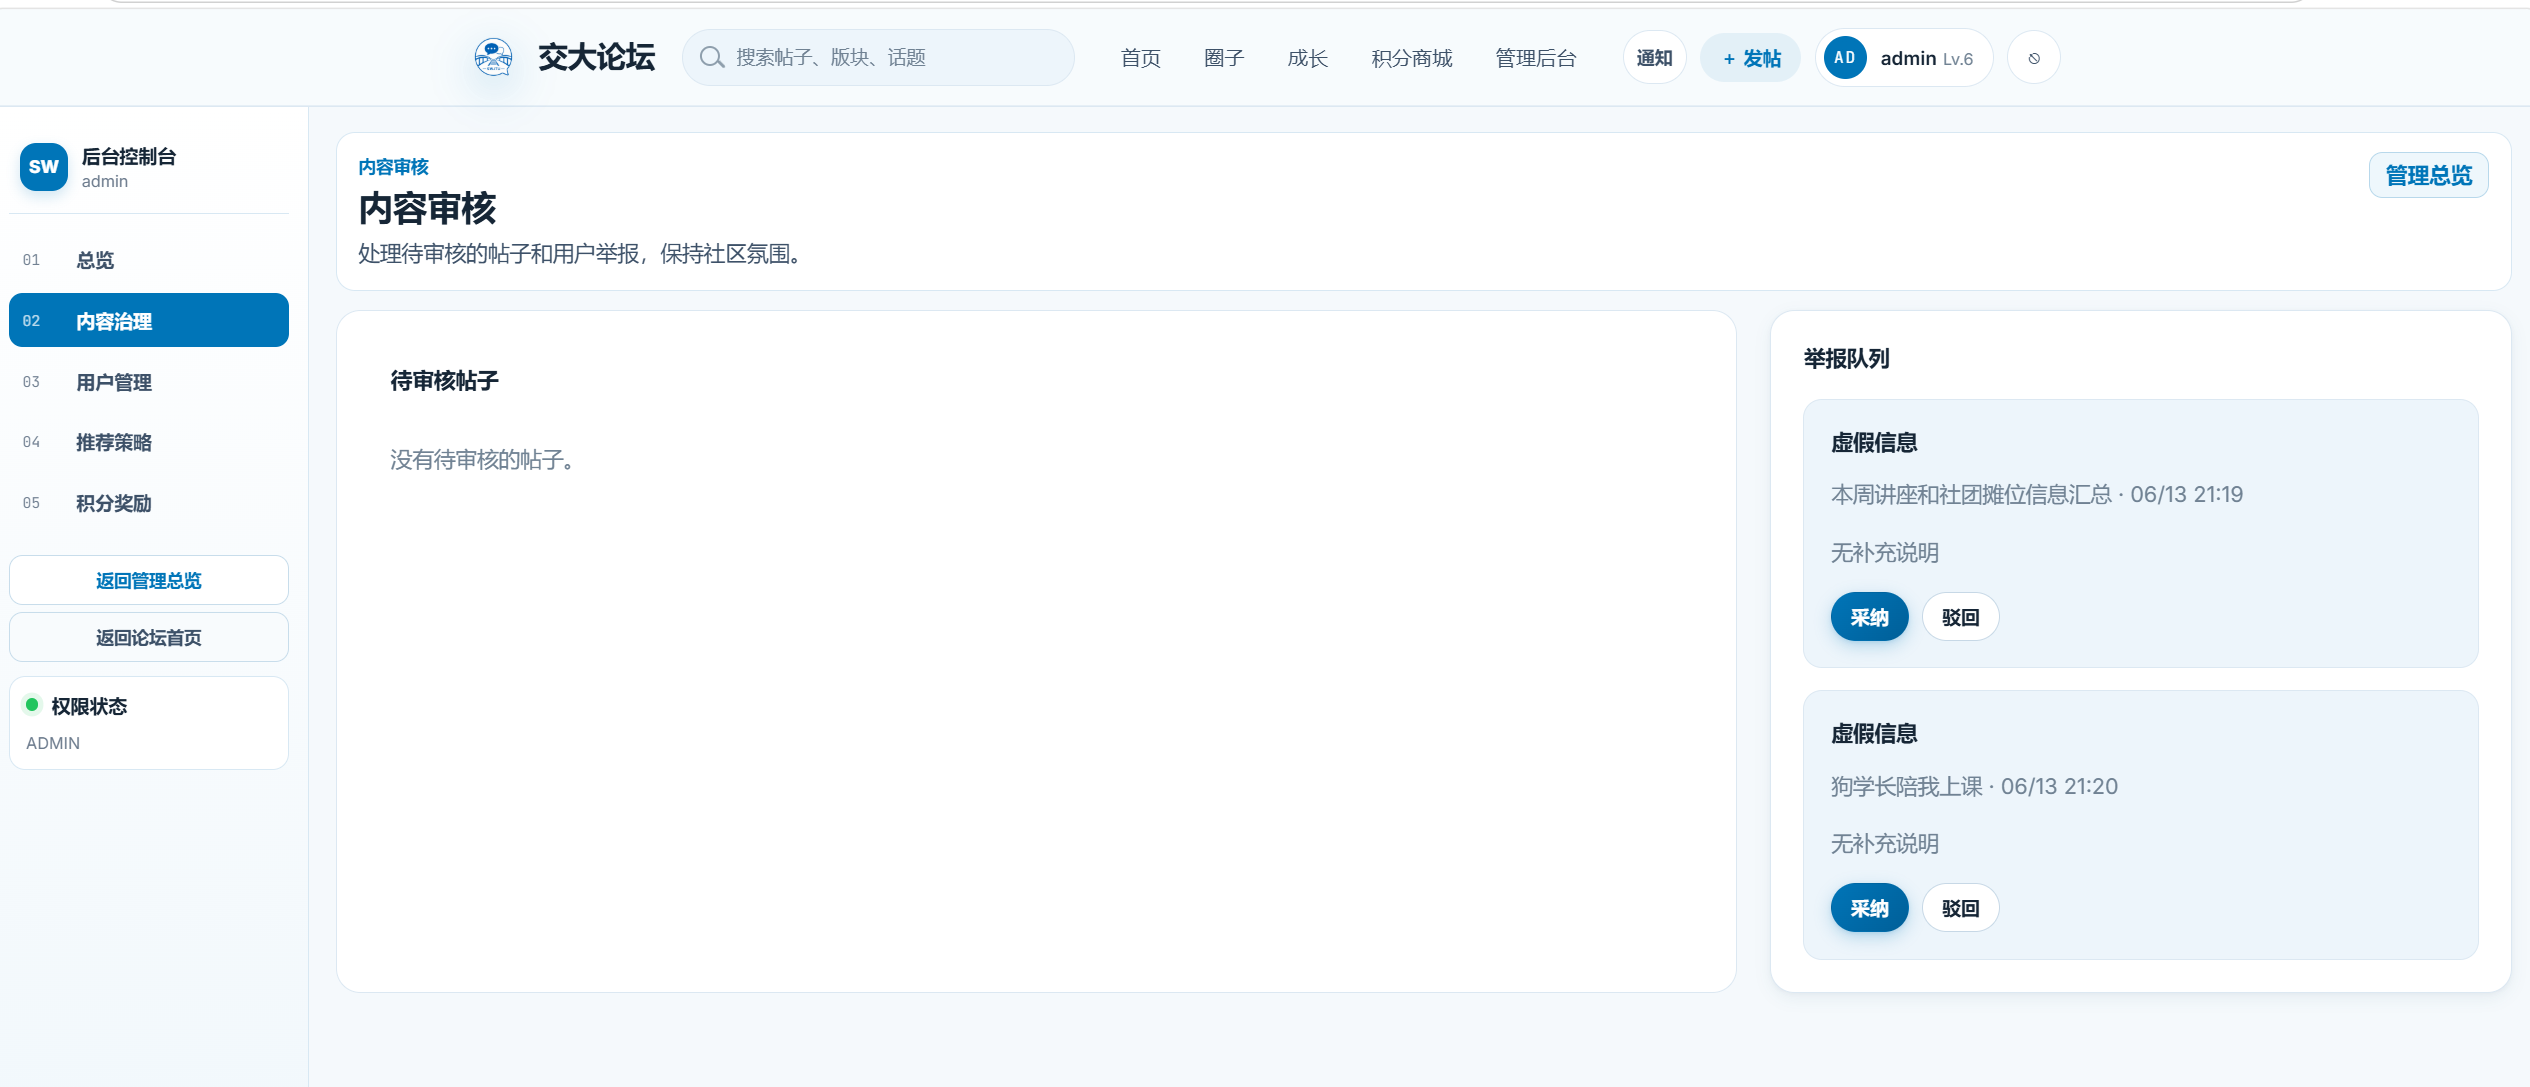
\includegraphics[width=0.92\textwidth]{figures/manual/comment_management.png}
    \caption{评论管理页面}
    \label{fig:comment-management}
\end{figure}

\subsection{用户管理与封禁}
「用户管理 $\rightarrow$ 用户列表」页面展示所有注册用户，支持按用户名、学号、认证状态、注册时间筛选。用户卡片展示：头像、昵称、学号、认证状态、注册时间、发帖数、等级、当前状态（正常/封禁）。

管理员操作：

\begin{itemize}[leftmargin=2em]
    \item \textbf{封禁账号}：将用户状态切换为「封禁」，被封禁用户无法正常登录和使用需要认证的论坛功能
    \item \textbf{解除封禁}：恢复被封禁用户的正常使用，用户状态变为「正常」
    \item \textbf{查看详情}：查看用户完整资料、发帖记录、评论记录、积分明细和操作日志
\end{itemize}



\begin{figure}[!htbp]
    \centering
    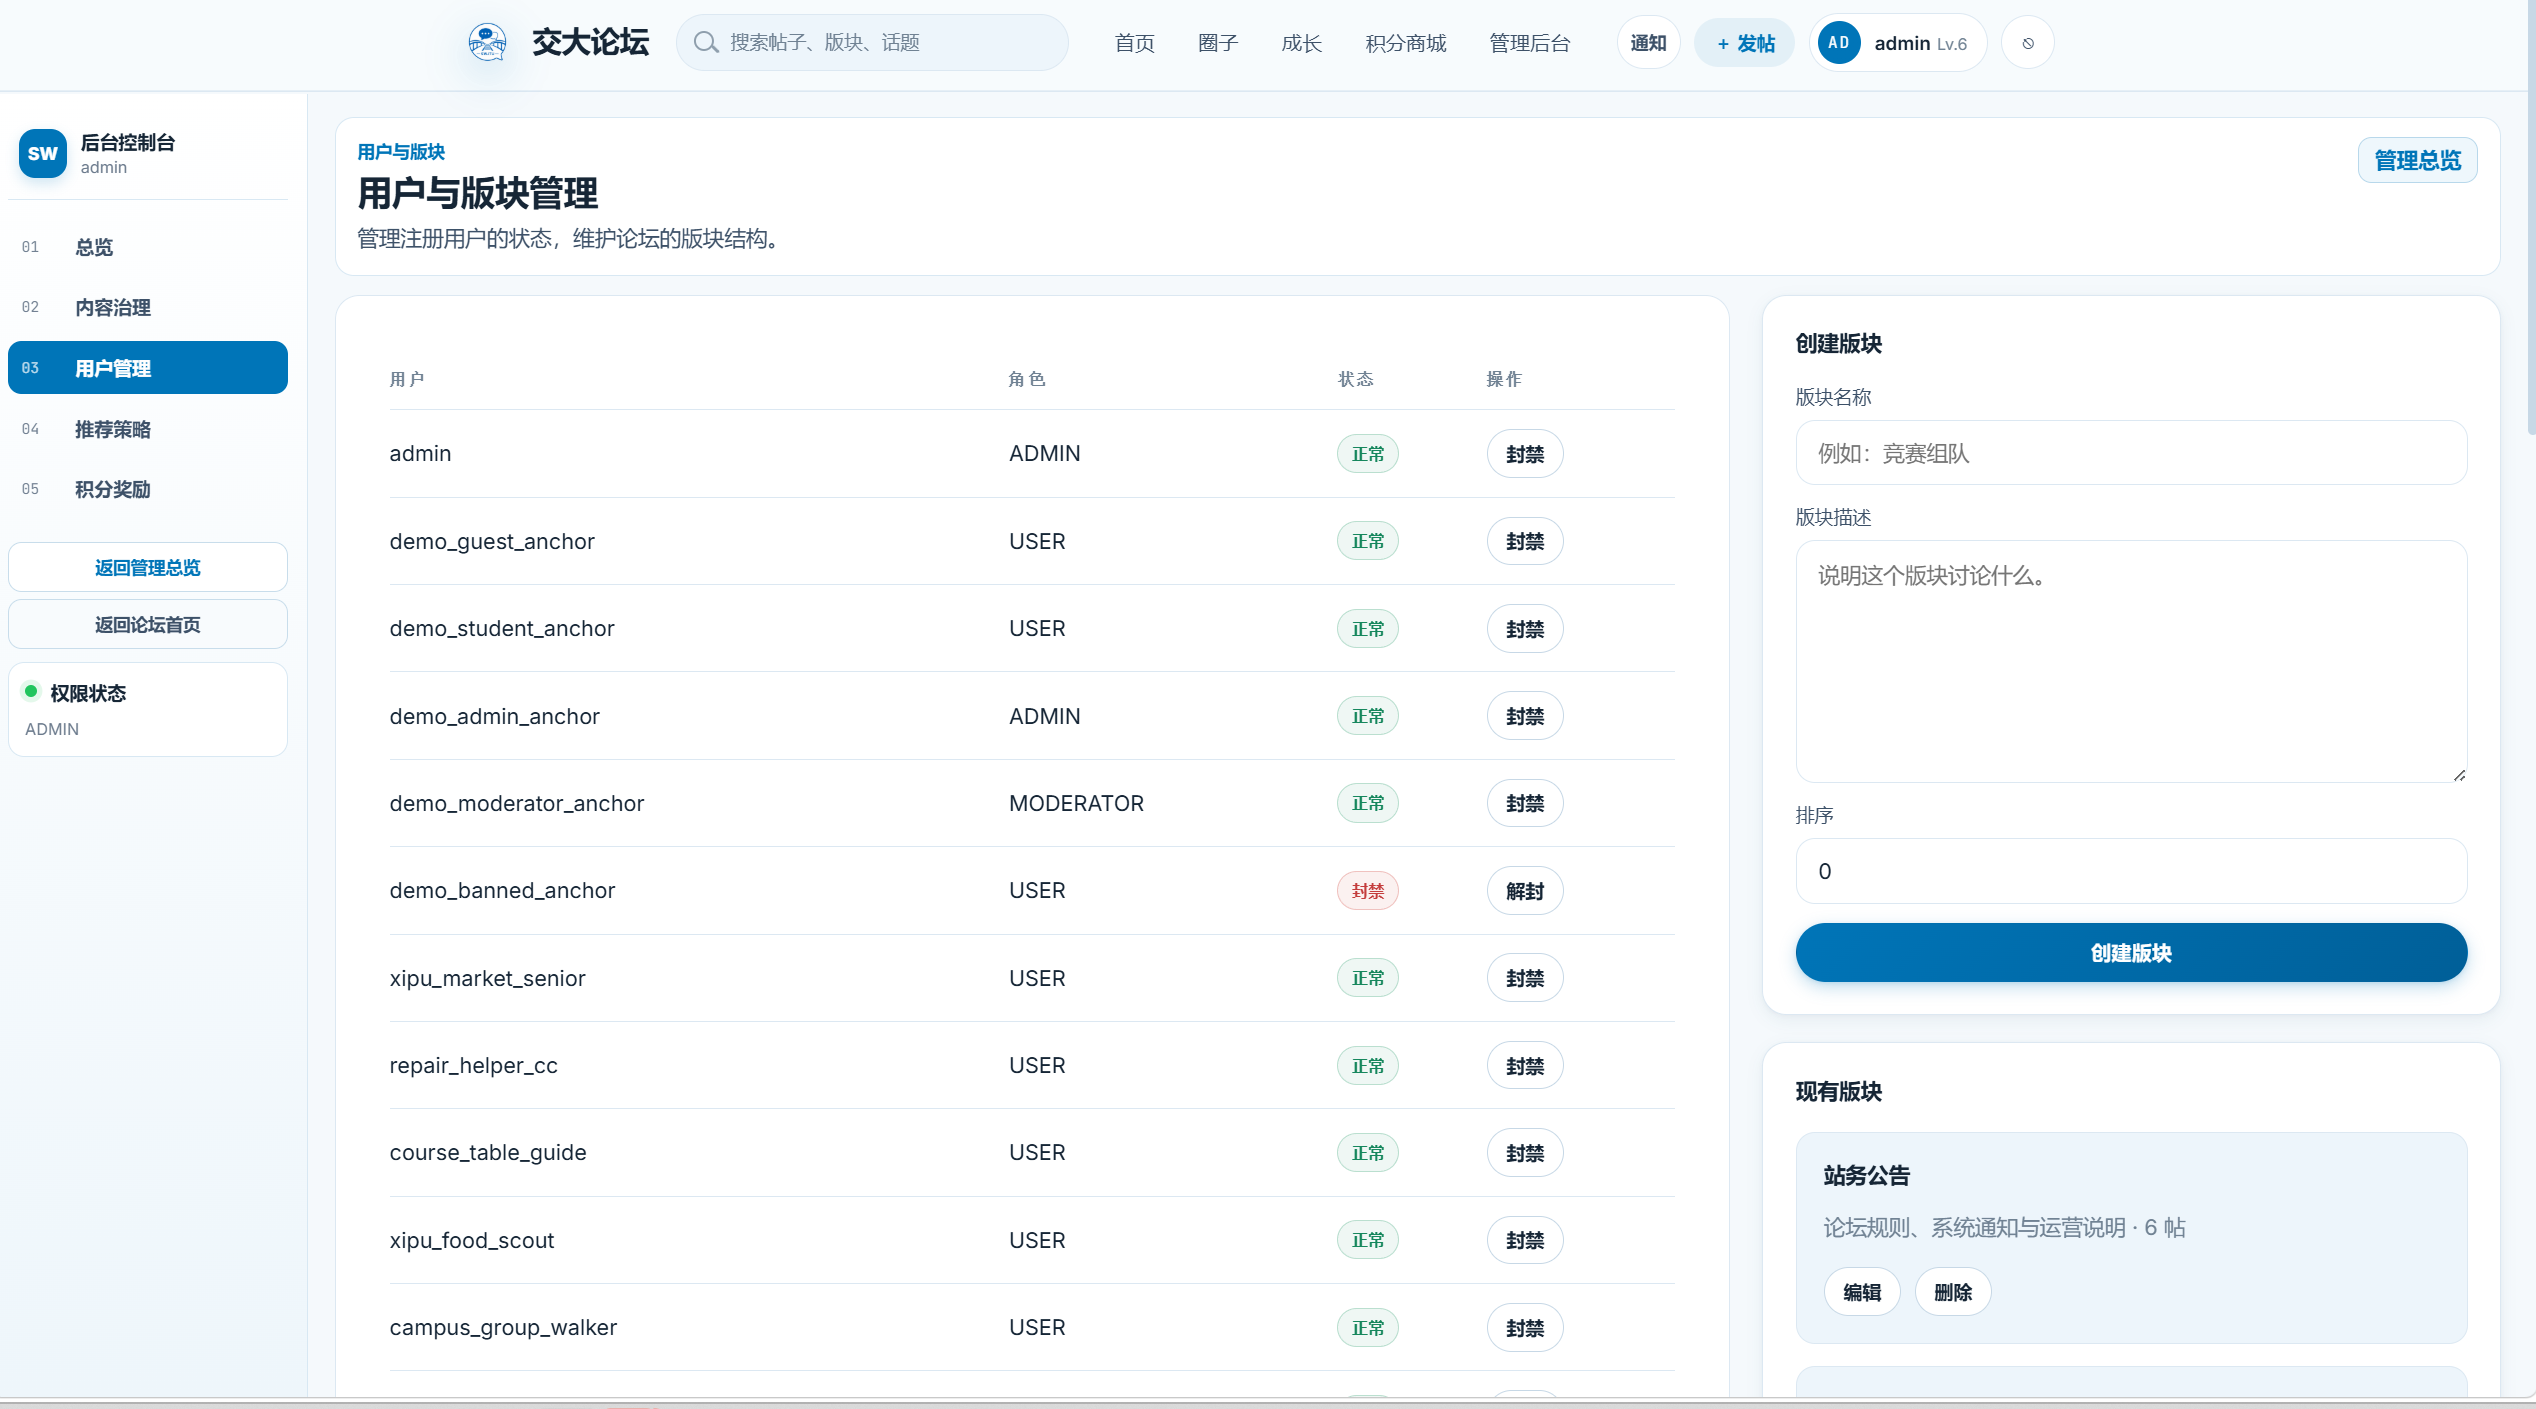
\includegraphics[width=0.92\textwidth]{figures/manual/user_management.png}
    \caption{用户管理与封禁页面}
    \label{fig:user-management}
\end{figure}

\subsection{举报处理}
「内容管理 $\rightarrow$ 举报处理」页面展示用户提交的举报列表，每行包含：举报类型（帖子/评论）、被举报内容摘要、举报原因、举报人、举报时间、处理状态（待处理/已采纳/已驳回）。管理员可逐条或批量处理：

\begin{itemize}[leftmargin=2em]
    \item \textbf{采纳举报}：被举报内容自动隐藏，通知举报人和被举报人处理结果
    \item \textbf{驳回举报}：举报不成立，通知举报人驳回原因
    \item \textbf{批量处理}：勾选多条举报，批量采纳或批量驳回
\end{itemize}


\begin{figure}[!htbp]
    \centering
    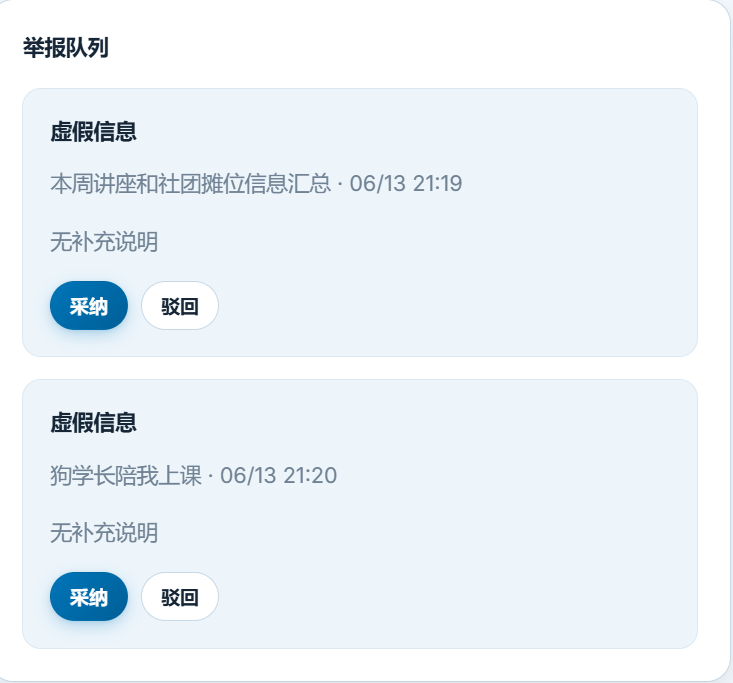
\includegraphics[width=0.92\textwidth]{figures/manual/report_management.png}
    \caption{举报处理页面}
    \label{fig:report-management}
\end{figure}

\subsection{版块管理}
「系统设置 $\rightarrow$ 版块管理」页面展示当前所有版块列表，管理员可进行：

\begin{itemize}[leftmargin=2em]
    \item \textbf{创建版块}：填写版块名称、描述、图标、排序权重、认证要求等属性
    \item \textbf{编辑版块}：修改版块属性，调整排序权重影响首页展示顺序
    \item \textbf{删除版块}：删除前需确认版块内无关联帖子，否则提示先迁移或删除帖子
\end{itemize}

版块属性包括：名称、描述、图标 URL、背景色、排序权重（数字越小越靠前）、认证要求（无/需认证）、发帖权限（所有人/认证用户/指定等级以上）。



\begin{figure}[!htbp]
    \centering
    \begin{subfigure}{0.48\textwidth}
        \centering
        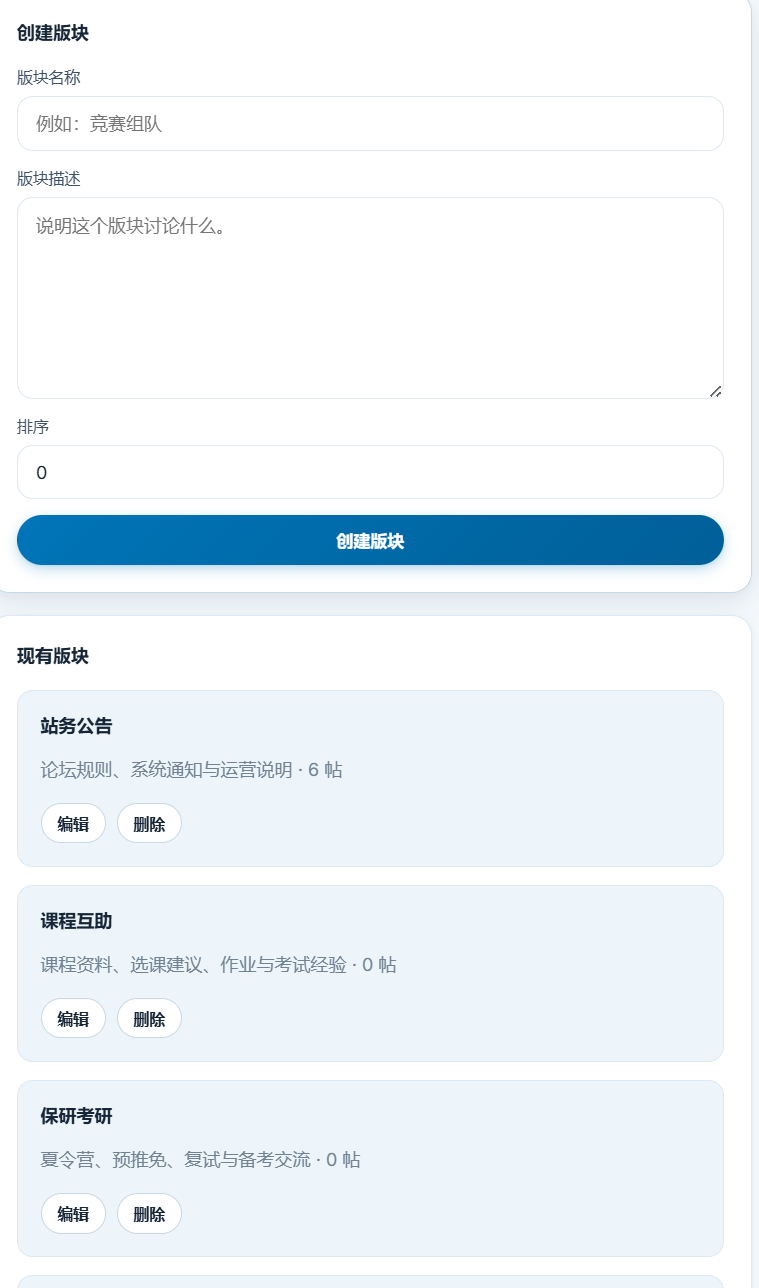
\includegraphics[width=\textwidth]{figures/manual/section_management.png}
        \caption{版块列表管理}
    \end{subfigure}
    \hfill
    \begin{subfigure}{0.48\textwidth}
        \centering
        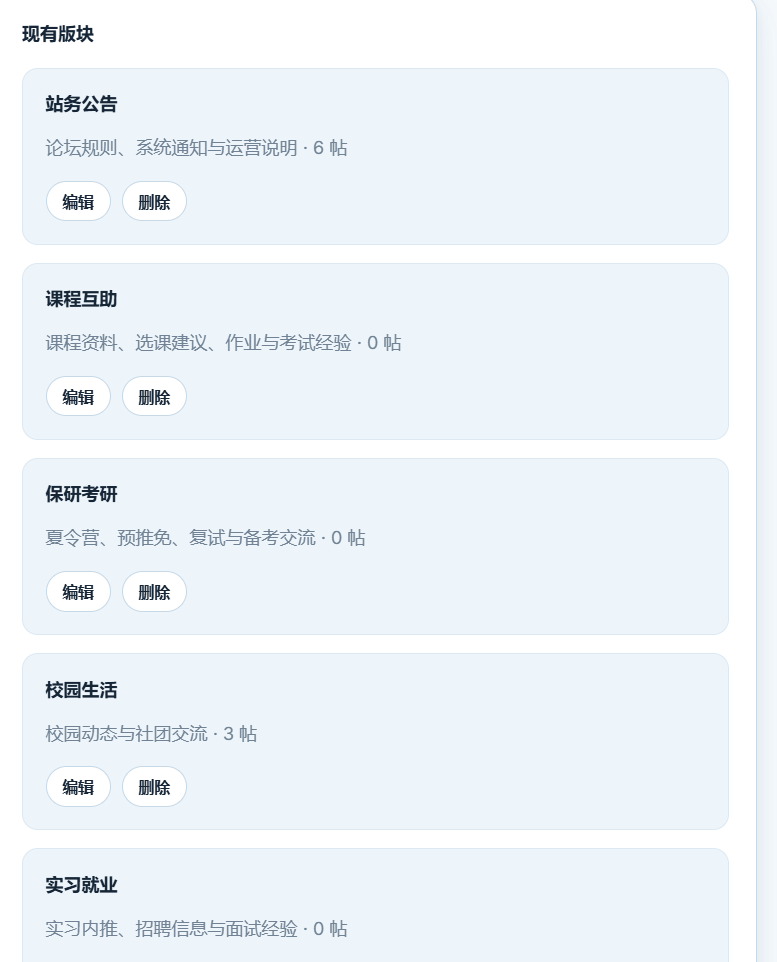
\includegraphics[width=\textwidth]{figures/manual/section_edit_form.png}
        \caption{版块编辑表单}
    \end{subfigure}
    \caption{版块管理功能}
    \label{fig:section-management}
\end{figure}

\subsection{积分兑换审核}
「运营管理 $\rightarrow$ 兑换审核」页面展示用户在积分商城提交的兑换申请列表，每行包含：申请人、奖品名称、积分价格、申请时间、收货地址（实物）、处理状态（待处理/已通过/已驳回）。管理员操作：

\begin{itemize}[leftmargin=2em]
    \item \textbf{通过}：虚拟奖品即时发放，实物奖品标记为「待发货」，通知用户处理结果
    \item \textbf{驳回}：填写驳回备注（如库存不足、地址不详），积分退还用户，通知用户原因
    \item \textbf{发货登记}：实物奖品通过快递发货后，填写物流公司和单号，用户可在「我的兑换」查看物流
\end{itemize}


\begin{figure}[!htbp]
    \centering
    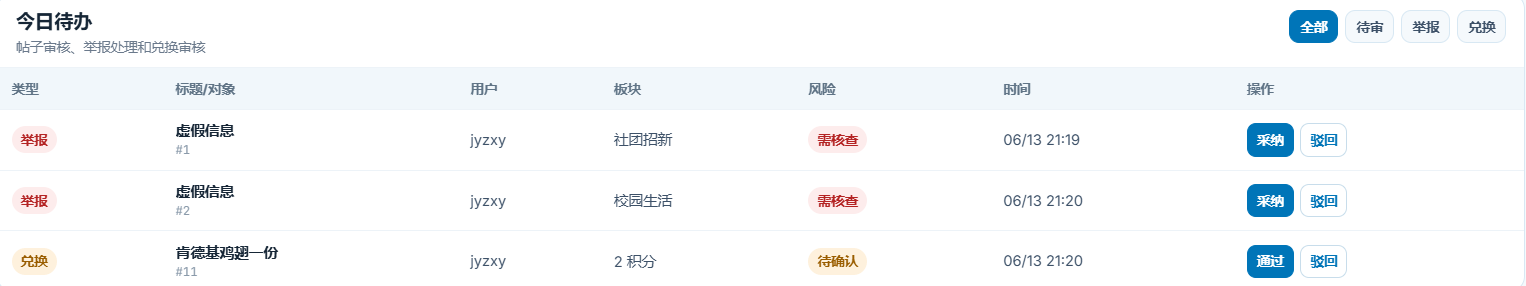
\includegraphics[width=0.92\textwidth]{figures/manual/exchange_audit.png}
    \caption{积分兑换审核页面}
    \label{fig:exchange-audit}
\end{figure}
\begin{figure}[!htbp]
	\centering
	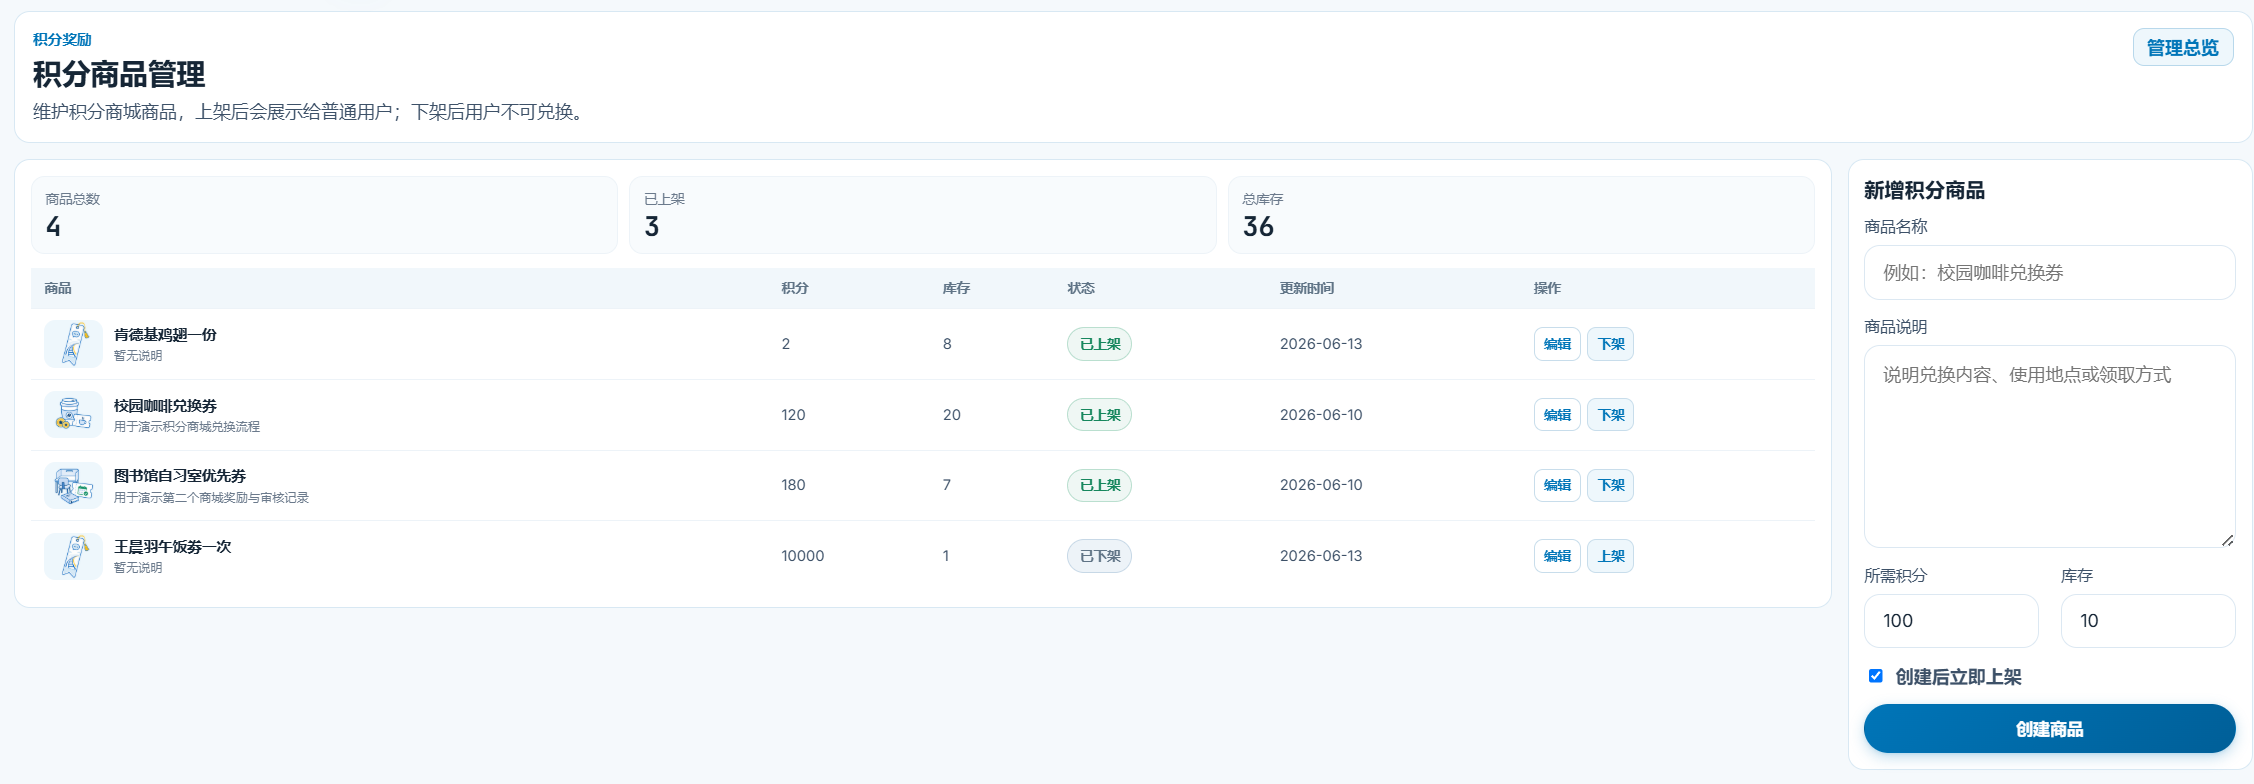
\includegraphics[width=0.92\textwidth]{figures/manual/exchange_audit1.png}
	\caption{积分兑换编辑页面}
	\label{fig:exchange-audit-detail}
\end{figure}

\subsection{推荐策略配置}
「系统设置 $\rightarrow$ 推荐配置」页面提供首页推荐算法的权重参数调整界面，管理员可拖动滑块或输入数值调整以下因素的权重：

\begin{itemize}[leftmargin=2em]
    \item \textbf{标签匹配权重}：用户兴趣标签与帖子标签的匹配度影响，默认 0.5
    \item \textbf{互动热度权重}：帖子互动数据（点赞、评论、收藏）的影响程度，默认 0.3
    \item \textbf{时间新鲜度权重}：基于用户历史行为的协同过滤推荐强度，默认 0.2
\end{itemize}

权重总和需等于 1.0，系统实时校验。调整后可点击「预览效果」查看模拟推荐结果，确认后点击「保存配置」生效。配置变更记录写入操作日志。


\begin{figure}[!htbp]
    \centering
    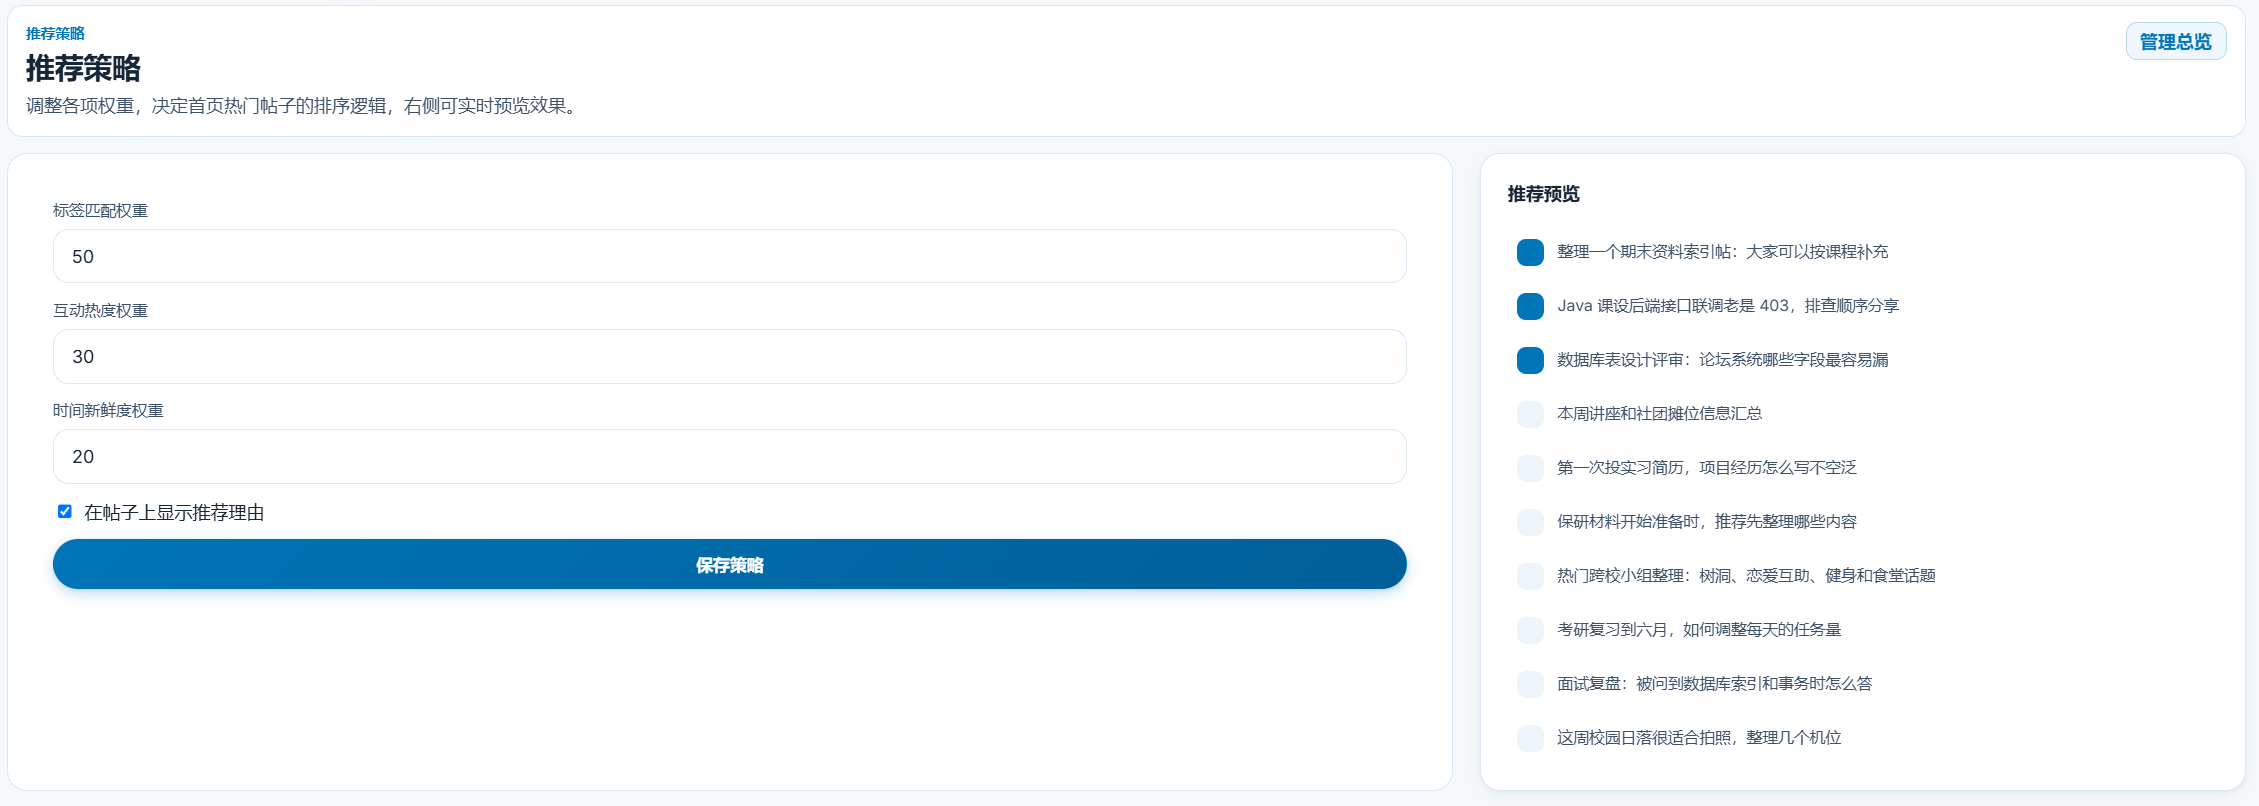
\includegraphics[width=0.92\textwidth]{figures/manual/recommend_config.png}
    \caption{推荐策略配置页面}
    \label{fig:recommend-config}
\end{figure}

\subsection{操作日志}
「系统设置 $\rightarrow$ 操作日志」页面自动记录管理员的所有操作，包括：操作时间、管理员账号、操作类型（封禁用户/删除帖子/审核通过/驳回举报等）、操作对象、操作详情、IP 地址。支持按时间范围、操作类型、管理员账号筛选。



\begin{figure}[!htbp]
    \centering
    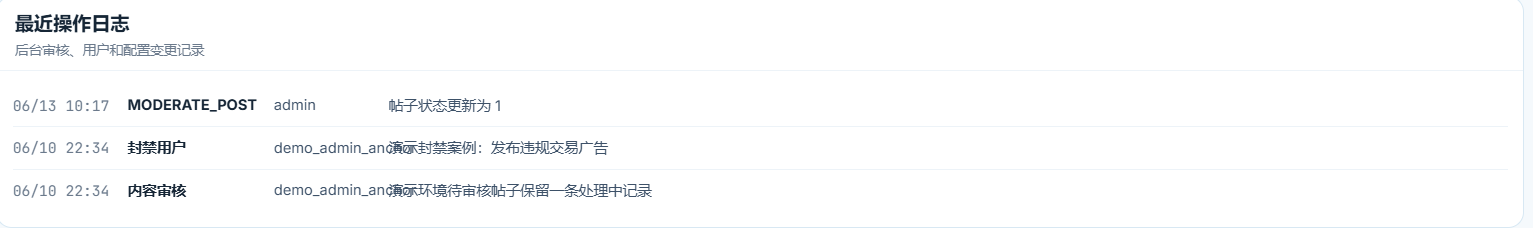
\includegraphics[width=0.92\textwidth]{figures/manual/operation_logs.png}
    \caption{操作日志页面}
    \label{fig:operation-logs}
\end{figure}

\section{常见问题}

\subsection{账号相关}
\textbf{Q1：如何注销账号？}

目前不支持自助注销。如需注销账号，请联系系统管理员，说明注销原因和账号信息，由管理员在后台核验后处理。注销或禁用后的账号数据处理以课程设计演示环境的管理规则为准。

\textbf{Q2：如何修改已发布的帖子？}

进入「个人中心 $\rightarrow$ 我的帖子」，找到目标帖子，点击「编辑」按钮。已发布帖子修改后需重新审核（已认证用户修改后即时生效）。注意：帖子被点赞或评论超过 10 次后，频繁修改可能影响阅读体验，建议谨慎编辑。

\textbf{Q3：头像上传失败怎么办？}

确保图片格式为 JPG 或 PNG，大小不超过 5MB。若仍失败，尝试压缩图片尺寸（建议 500$\times$500 像素以上但不超过 2000$\times$2000 像素），或更换浏览器（推荐 Chrome/Firefox/Edge 最新版）。

\subsection{积分与等级}

\textbf{Q4：积分不够兑换奖品怎么办？}

多参与论坛互动获取积分：每日签到（5--15 分）、发布优质帖子（10--30 分）、积极评论（2--5 分/条）、收藏帖子（1 分/条，上限 10 分/日）。完成校园认证可一次性获得 100 积分，且每日积分上限提升至 80 分。

\textbf{Q5：发帖后没有显示？}

新发布帖子需经过审核（未认证用户）或直接发布（已认证用户）。审核通常在 5--30 分钟内完成，可在「个人中心 $\rightarrow$ 我的帖子」查看审核状态。若长时间未审核，请联系管理员。

\subsection{技术问题}

\textbf{Q6：页面加载缓慢或显示异常？}

尝试以下步骤：清除浏览器缓存（Ctrl+Shift+Delete）并刷新页面（F5）；检查网络连接；更换浏览器或更新至最新版本；禁用浏览器插件（尤其是广告拦截插件）。若问题持续，请通过「意见反馈」入口提交问题描述和截图。



\section{总结}

本文围绕西南交大校园论坛系统，从用户视角和管理员视角两个维度，详细说明了系统的各项功能与操作流程。用户端功能涵盖注册登录、内容浏览、发帖互动、积分成长、个人管理和社交关注；管理端功能涵盖数据统计、内容审核、用户管理、举报处理、版块配置和运营策略调整。

通过逐项功能说明与界面截图指导，本文旨在帮助用户快速上手论坛系统，同时为开发团队提供完整的功能验收依据。后续版本迭代中，建议优先完善移动端适配、消息实时推送、智能内容审核和个性化推荐算法优化，以进一步提升用户体验和平台运营效率。

\end{document}
